% Este trabajo está alojado en un repositorio git:
% \url{https://github.com/CarlosJEugenio/Tesis}
% Carlos Eugenio 2018

\documentclass[aspectratio=169]{beamer}
\usetheme{metropolis}           % Use metropolis theme
\usepackage[utf8]{inputenc}
\usepackage[spanish]{babel}
\usepackage{subcaption}
%%package para bibliografía
\usepackage{natbib}
\usepackage[american,siunitx]{circuitikz}
\usepackage[version=4]{mhchem}
\usepackage{caption}
\captionsetup{font=scriptsize,labelfont=scriptsize}
\captionsetup[subfigure]{font=scriptsize,labelfont=scriptsize}
\usepackage{pgfplots}
\usepackage{pgfplotstable,tabularx,booktabs}
\usepackage[]{qrcode}
\usepackage{gensymb}

\usetikzlibrary{positioning}
%\usetikzlibrary{pgfplots.clickable}
%\usepgfplotslibrary{clickable}
\usepgfplotslibrary{units}
\usepackage{multirow}
\usepackage{xcolor,colortbl}
\definecolor{LightCyan}{rgb}{0.88,1,1}

\let\clipbox\relax
\usepackage{adjustbox}

\newcommand{\plotwidth}{0.2\textwidth}
\newcommand{\plotscale}{0.8}

\captionsetup{subrefformat=parens}

\setbeamercovered{invisible}
%\setbeamercovered{%
%	again covered={\opaqueness<1->{10}}}
\usepackage[skins]{tcolorbox}
\graphicspath{{Imagenes/}}

\tikzset{
	invisible/.style={opacity=0},
	visible on/.style={alt={#1{}{invisible}}},
	alt/.code args={<#1>#2#3}{%
		\alt<#1>{\pgfkeysalso{#2}}{\pgfkeysalso{#3}} % \pgfkeysalso doesn't change the path
	},
}

%nombre de muestras:
\newcommand{\mSustratoAcero}{SusAc }
\newcommand{\mPolvoAcero}{PolvoAc }
\newcommand{\mPolvoAceroPMMA}{PolvoAc+pmma }
\newcommand{\mPapelAcero}{PapelAc }
\newcommand{\mLiofilizadoAcero}{LioAc }
\newcommand{\mSustratoNiquel}{SusNi }
\newcommand{\mPolvoNiquel}{PolvoNi }
\newcommand{\mPolvoNiquelPMMA}{PolvoNi+pmma }

\definecolor{RYB1}{RGB}{228,26,28}
\definecolor{RYB2}{RGB}{55,126,184}
\definecolor{RYB3}{RGB}{77,175,74}
\definecolor{RYB4}{RGB}{152,78,163}
\definecolor{RYB5}{RGB}{255,127,0}
\definecolor{RYB6}{RGB}{255,255,51}
\definecolor{RYB7}{RGB}{166,86,40}
\definecolor{ce4edc3}{RGB}{228,237,195}
\definecolor{cfe9999}{RGB}{254,153,153}
\definecolor{c575757}{RGB}{87,87,87}
\definecolor{c43d8ff}{RGB}{67,216,255}
\definecolor{c323232}{RGB}{50,50,50}
\definecolor{c71d89a}{RGB}{113,216,154}
\definecolor{cbfbfbf}{RGB}{191,191,191}
\definecolor{c252525}{RGB}{37,37,37}
\definecolor{red_oxigen}{RGB}{211,95,95}

\definecolor{samplegreen}{RGB}{150,250,150}

\pgfplotscreateplotcyclelist{colorbrewer-RYB}{
	{RYB1},every mark/.append style={fill=RYB1!80!black},mark=*\\
	{RYB2},every mark/.append style={fill=RYB2!80!black},mark=square*\\
	{RYB3},every mark/.append style={fill=RYB3!80!black},mark=diamond*\\
	{RYB4},every mark/.append style={fill=RYB4!80!black},mark=triangle*\\
	{RYB5},every mark/.append style={fill=RYB5!80!black},mark=pentagon*\\
	{RYB6},every mark/.append style={fill=RYB6!80!black},mark=o\\
	{RYB7},every mark/.append style={fill=RYB7!80!black},mark=square\\
}


\pgfplotsset{
	compat=1.15,
	CVStyle/.style={
		title=Voltametría Cíclica,
		domain=-0.8:0.8,
		xtick distance=0.4,
		minor tick num=1,
		ylabel={Densidad de corriente [A/g]},
		xlabel={Voltaje [V]},
		every axis legend/.append style={
			font=\normalsize,
			at={(0.98,0.02)},
			anchor=south east,
		},
		legend entries={25mV/s,50mV/s,100mV/s,200mV/s,400mV/s},
		cycle list name=colorbrewer-RYB,
		no markers,
		thick,
	},
	SCStyle/.style={
		title=Capacidad Específica,
		domain=25:400,
		ylabel={Capacidad específica [F/g]},
		xlabel={Velocidad de barrido [mV/s]},
		every axis legend/.append style={
			font=\normalsize,
			at={(0.98,0.98)},
			anchor=north east,
		},
		legend entries={Antes, Después},
		cycle list name=colorbrewer-RYB,
		every mark/.append style={
			fill opacity=0.5,
			draw opacity=0.5,}
	},
	EISStyle/.style={
		title=Espectro de impedancia electroquímica,
		domain=0:50,
		ylabel={-Z imag [$\Omega$]},
		xlabel={Z real [Ohm]},
		cycle list name=colorbrewer-RYB,	
	},
	CCDStyle/.style={
		title=Carga y descarga cíclica,
		ylabel={Voltaje [V]},
		xlabel={Tiempo [s]},
		cycle list name=colorbrewer-RYB,
		mark size = 1pt,
		line width = 0.1pt,
		%		only markers,
		every axis legend/.append style={
			font=\normalsize,
			at={(0.98,0.02)},
			anchor=south east,
		},
		legend entries={Primeros ciclos, Últimos ciclos},
	},
}

\pgfplotsset{
	/pgfplots/bar  cycle  list/.style={/pgfplots/cycle  list={%
			{RYB1,fill=RYB1!80!black,mark=*},
			{RYB2,fill=RYB2!80!black,mark=square*},
			{RYB3,fill=RYB3!80!black,mark=diamond*},
			{RYB4,fill=RYB4!80!black,mark=triangle*},
			{RYB5,fill=RYB5!80!black,mark=*},
			{RYB6,fill=RYB6!80!black,mark=square*},
			{RYB7,fill=RYB7!80!black,mark=diamond*},
		}
	},
}
\title{Síntesis de grafeno por medios químicos\\y supercondensadores basados en grafeno}
\date{\today}
\institute{Universidad de Santiago de Chile\\ Laboratorio de Nanosíntesis}
\begin{document}
	\author[Carlos Eugenio]{\begin{tabular}{r@{ }l} 
			Autor:      & Carlos Eugenio \\[1ex] 
			Profesor guía: & Dinesh Pratap Singh
	\end{tabular}}
	\maketitle
	\begin{frame}
		\frametitle{Table of Contents}
		\tableofcontents
	\end{frame}

	\section{Objetivos}
	\begin{frame}{Objetivos}
		\uncover<1->{
			\textbf{Objetivo general:}
			\begin{itemize}
				\item Sintetizar \textbf{óxido de grafeno reducido}, para su utilización en electrodos de \textbf{supercondensadores}.
			\end{itemize}}
		\uncover<2->{
			\textbf{Objetivo en el laboratorio:}
			\begin{itemize}
				\item Implementar una \textbf{metodología} para \textbf{construir y caracterizar supercondensadores}.
			\end{itemize}}
	\end{frame}

	\begin{frame}{Objetivos}
		\textbf{Objetivos específicos:}
		\begin{itemize}[<+->]
			\item Sintetizar \textbf{óxido de grafeno (GO)}, a partir de grafito natural mediante un proceso químico; para su posterior reducción y obtención de \textbf{óxido reducido de grafeno (rGO)}.
			\item Fabricar electrodos de \textbf{óxido de grafeno reducido} con diferentes métodos, para su posterior caracterización electroquímica.
			\item Diseñar y construir una \textbf{celda de pruebas de supercondensadores} para estudiar el desempeño de diferentes electrodos fabricados.
			\item Elaborar una \textbf{metodología de medición electroquímica} para cuantificar y comparar el desempeño de los diferentes electrodos fabricados. 
		\end{itemize}
	\end{frame}

	\section{Introducción}
	\subsection{Supercondensadores}
	\begin{frame}{¿Por qué usar supercondensadores?}
		\begin{columns}
			\begin{column}{0.5\textwidth}
				\only<1->\textbf{¿Qué es un supercondensador?}
				\begin{itemize}[<+(1)->]
					\item Es un dispositivo eléctrico de \textbf{almacenamiento de energía}.
					\item Parecido a una batería.
					\item Pero \textbf{más parecido a un condensador convencional}.
				\end{itemize}
			\end{column}
			\begin{column}{0.5\textwidth}
				\begin{onlyenv}<1-4>
					\begin{figure}[b]
						\begin{tikzpicture}
							\node at (3,2) {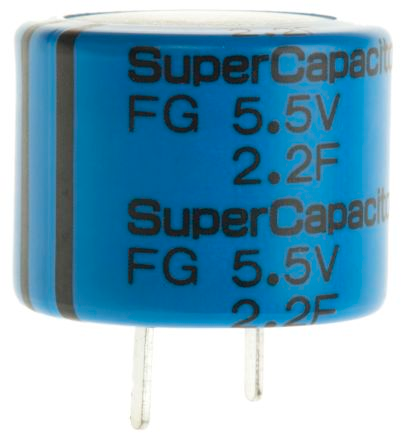
\includegraphics[width=0.3\textwidth]{com_sc_1.png}};
							\node at (0,2) {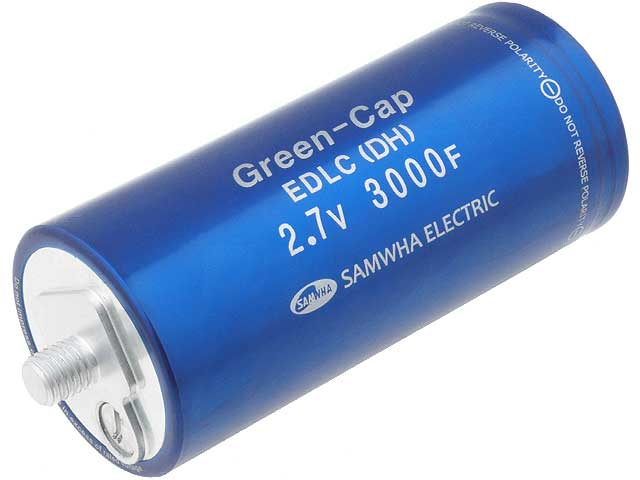
\includegraphics[width=0.5\textwidth]{com_sc_2.png}};
							\node at (1,-1) {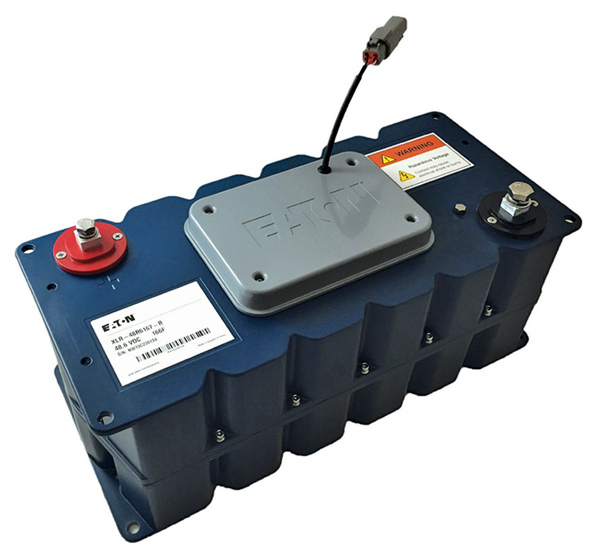
\includegraphics[width=0.6\textwidth]{com_sc_3.png}};
						\end{tikzpicture}
						\caption{Supercondensadores comercialmente disponibles.}
					\end{figure}
				\end{onlyenv}

			\end{column}
		\end{columns}
	\end{frame}

	\begin{frame}{¿Por qué usar supercondensadores?}
		\begin{columns}
			\begin{column}{0.5\textwidth}
				\only<1->\textbf{En términos energéticos:}
				\begin{itemize}[<+(1)->]
					\item Puede almacenar y entregar energía \textbf{más rápido que una batería}, y de forma \textbf{más eficiente}.
					\item Pero en \textbf{menor cantidad}.
					\item Son idóneos para aplicaciones que requieran \textbf{respuestas rápidas por un corto periodo de tiempo}.
					\item \textbf{Frenado regenerativo}, \textbf{sistemas de respaldo}, \textbf{recolección de energía}, etc.
				\end{itemize}
			\end{column}
			\begin{column}{0.5\textwidth}
				\begin{figure}[b]
					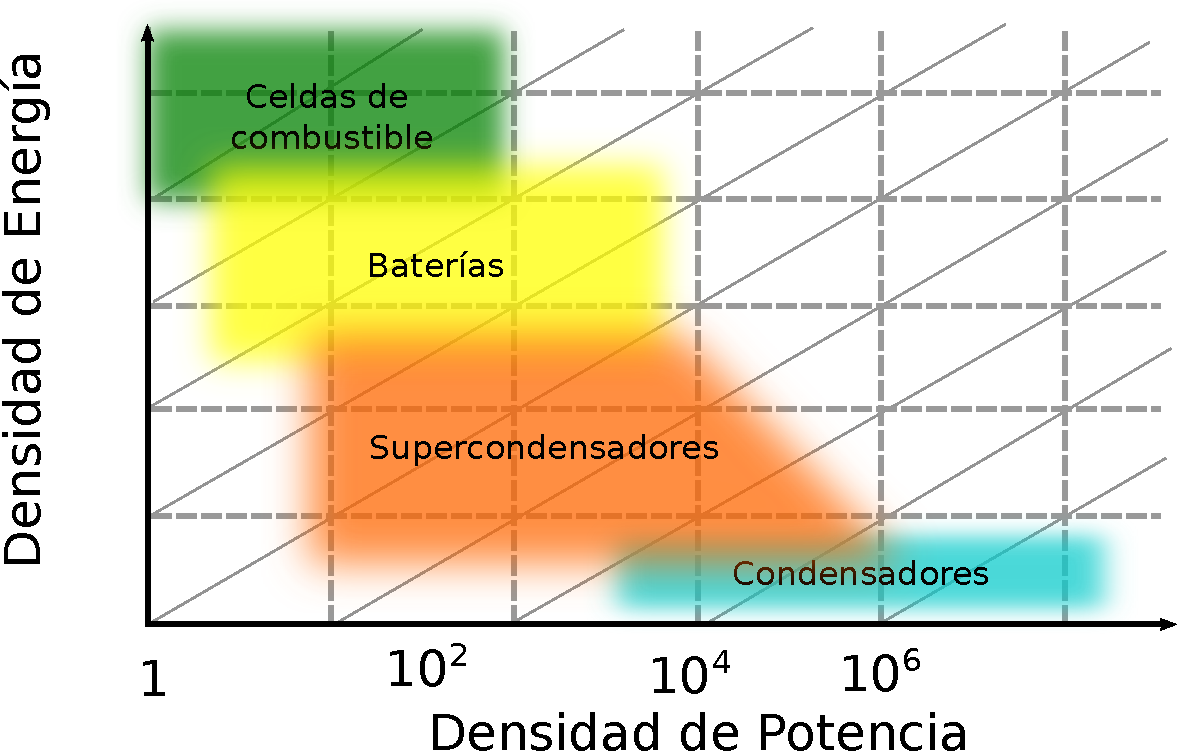
\includegraphics[width = \textwidth]{ragone.pdf}
					\caption{Diagrama de Ragone}
				\end{figure}
			\end{column}
		\end{columns}
	\end{frame}

%	\begin{frame}
%		\begin{columns}
%			\begin{column}{0.5\textwidth}
%
%			\end{column}
%			\begin{column}{0.5\textwidth}
%
%			\end{column}
%		\end{columns}
%	\end{frame}

	\begin{frame}{El supercondensador}
		\begin{columns}
			\begin{column}{0.5\textwidth}
				\only<1->\textbf{¿Cómo funciona un supercondensador?}
				\begin{itemize}
					\item<2-> Un sándwich de dos \textbf{electrodos}, con un \textbf{separador} empapado de \textbf{electrolito} en medio.
					\item<3-> Almacena energía mediante separación de cargas en una \textbf{doble capa eléctrica}.
					\item<4-> Esta doble capa tiene \textbf{pocos nanómetros de espesor}.
				\end{itemize}
			\end{column}
			\begin{column}{0.5\textwidth}
				\begin{figure}[h!]
					\centering
					\begin{tikzpicture}
					\node at (0,0) {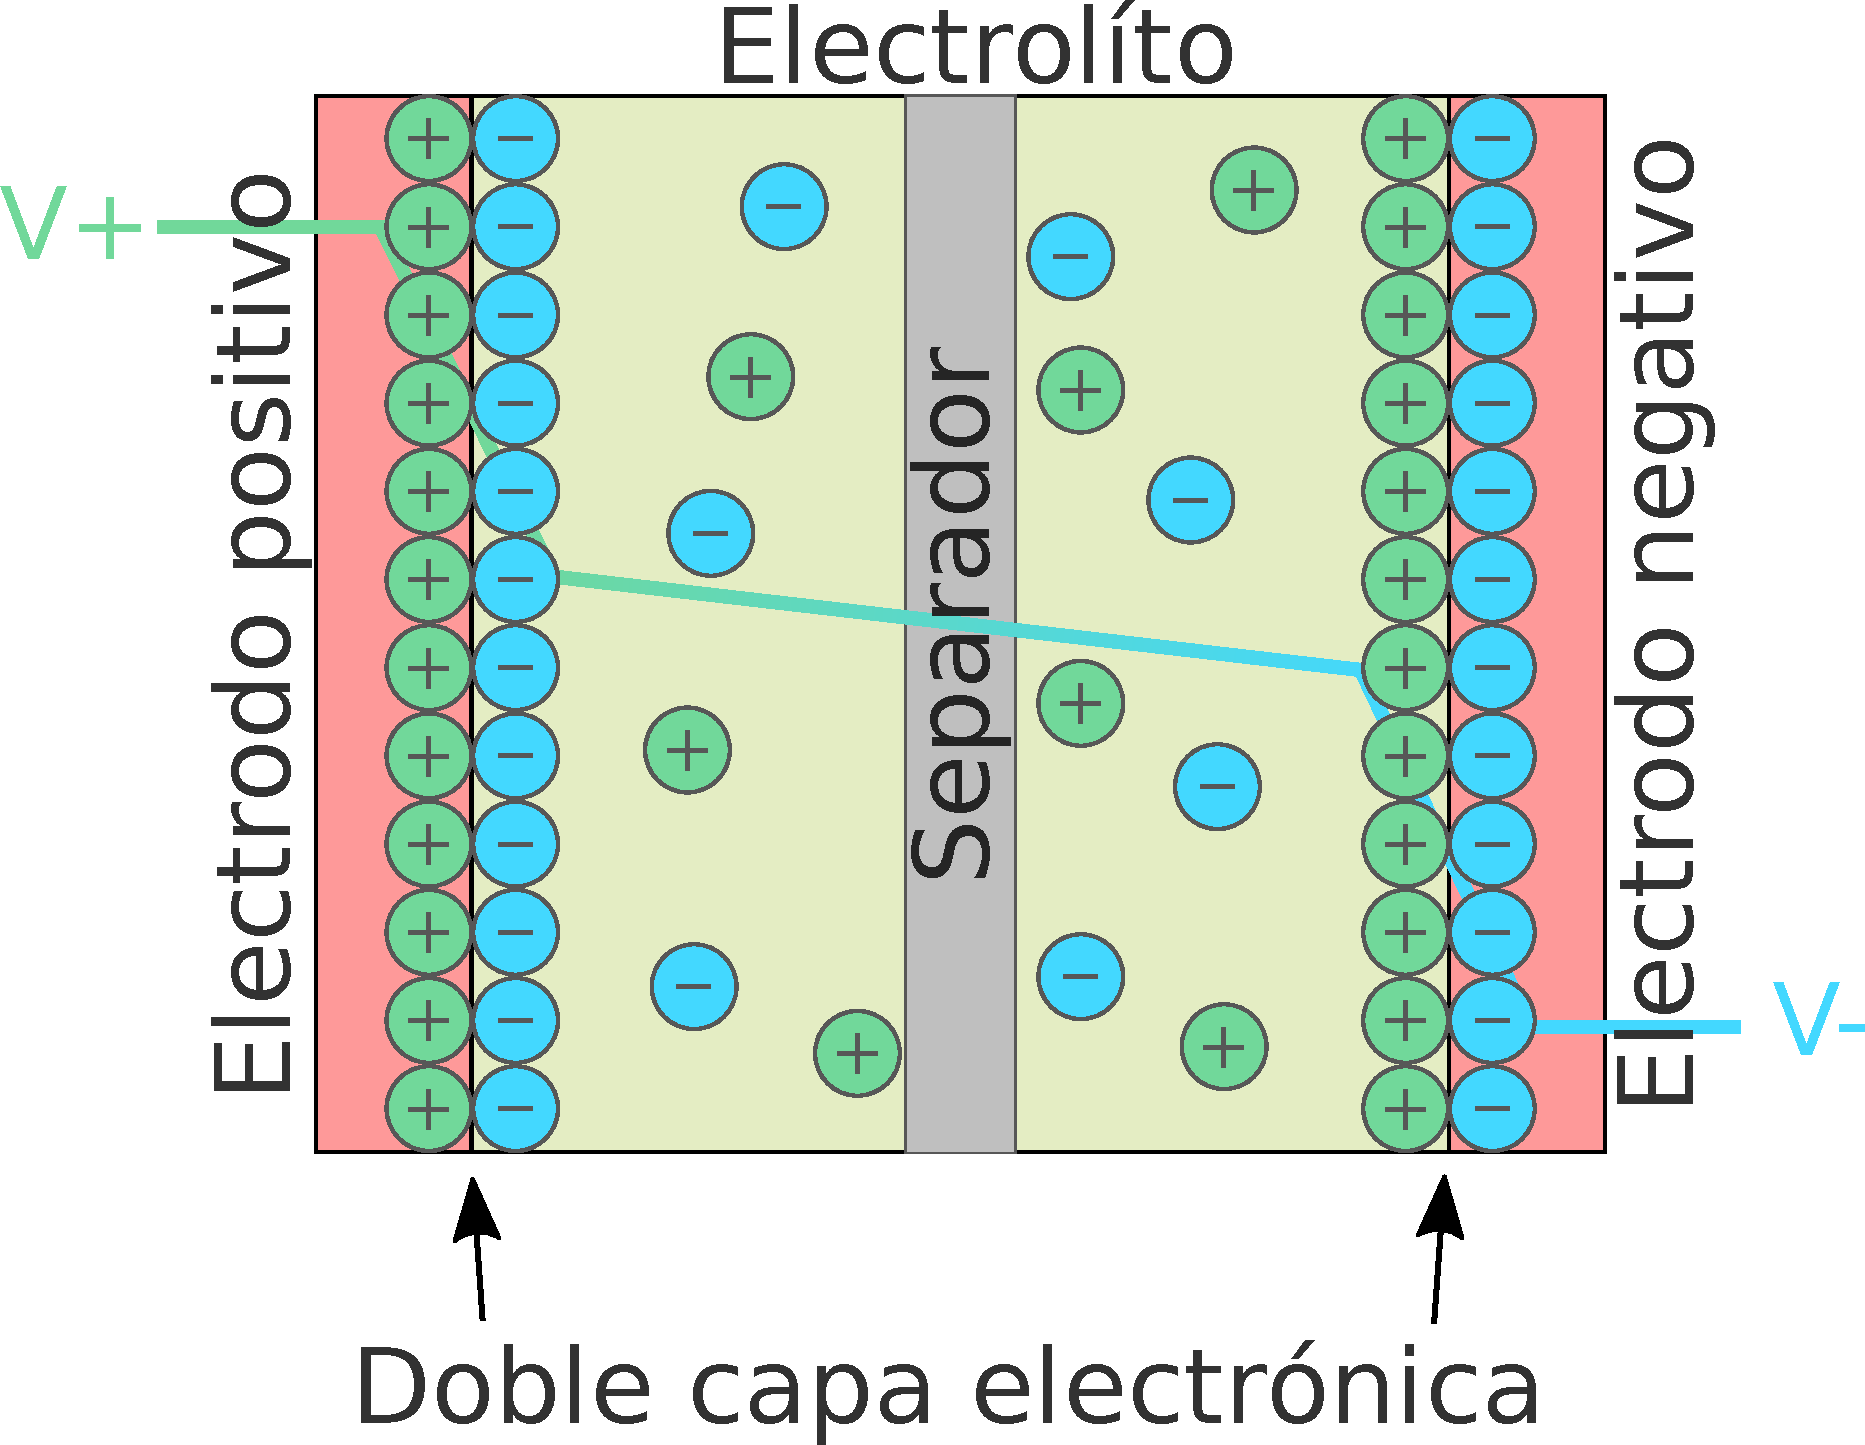
\includegraphics[width=\textwidth]{edlc_schem.pdf}};
					\only<4>{\begin{scope}
						\clip[draw] (-1.6, 0.2) circle(2cm);
						\node at (-1.5,0.5) {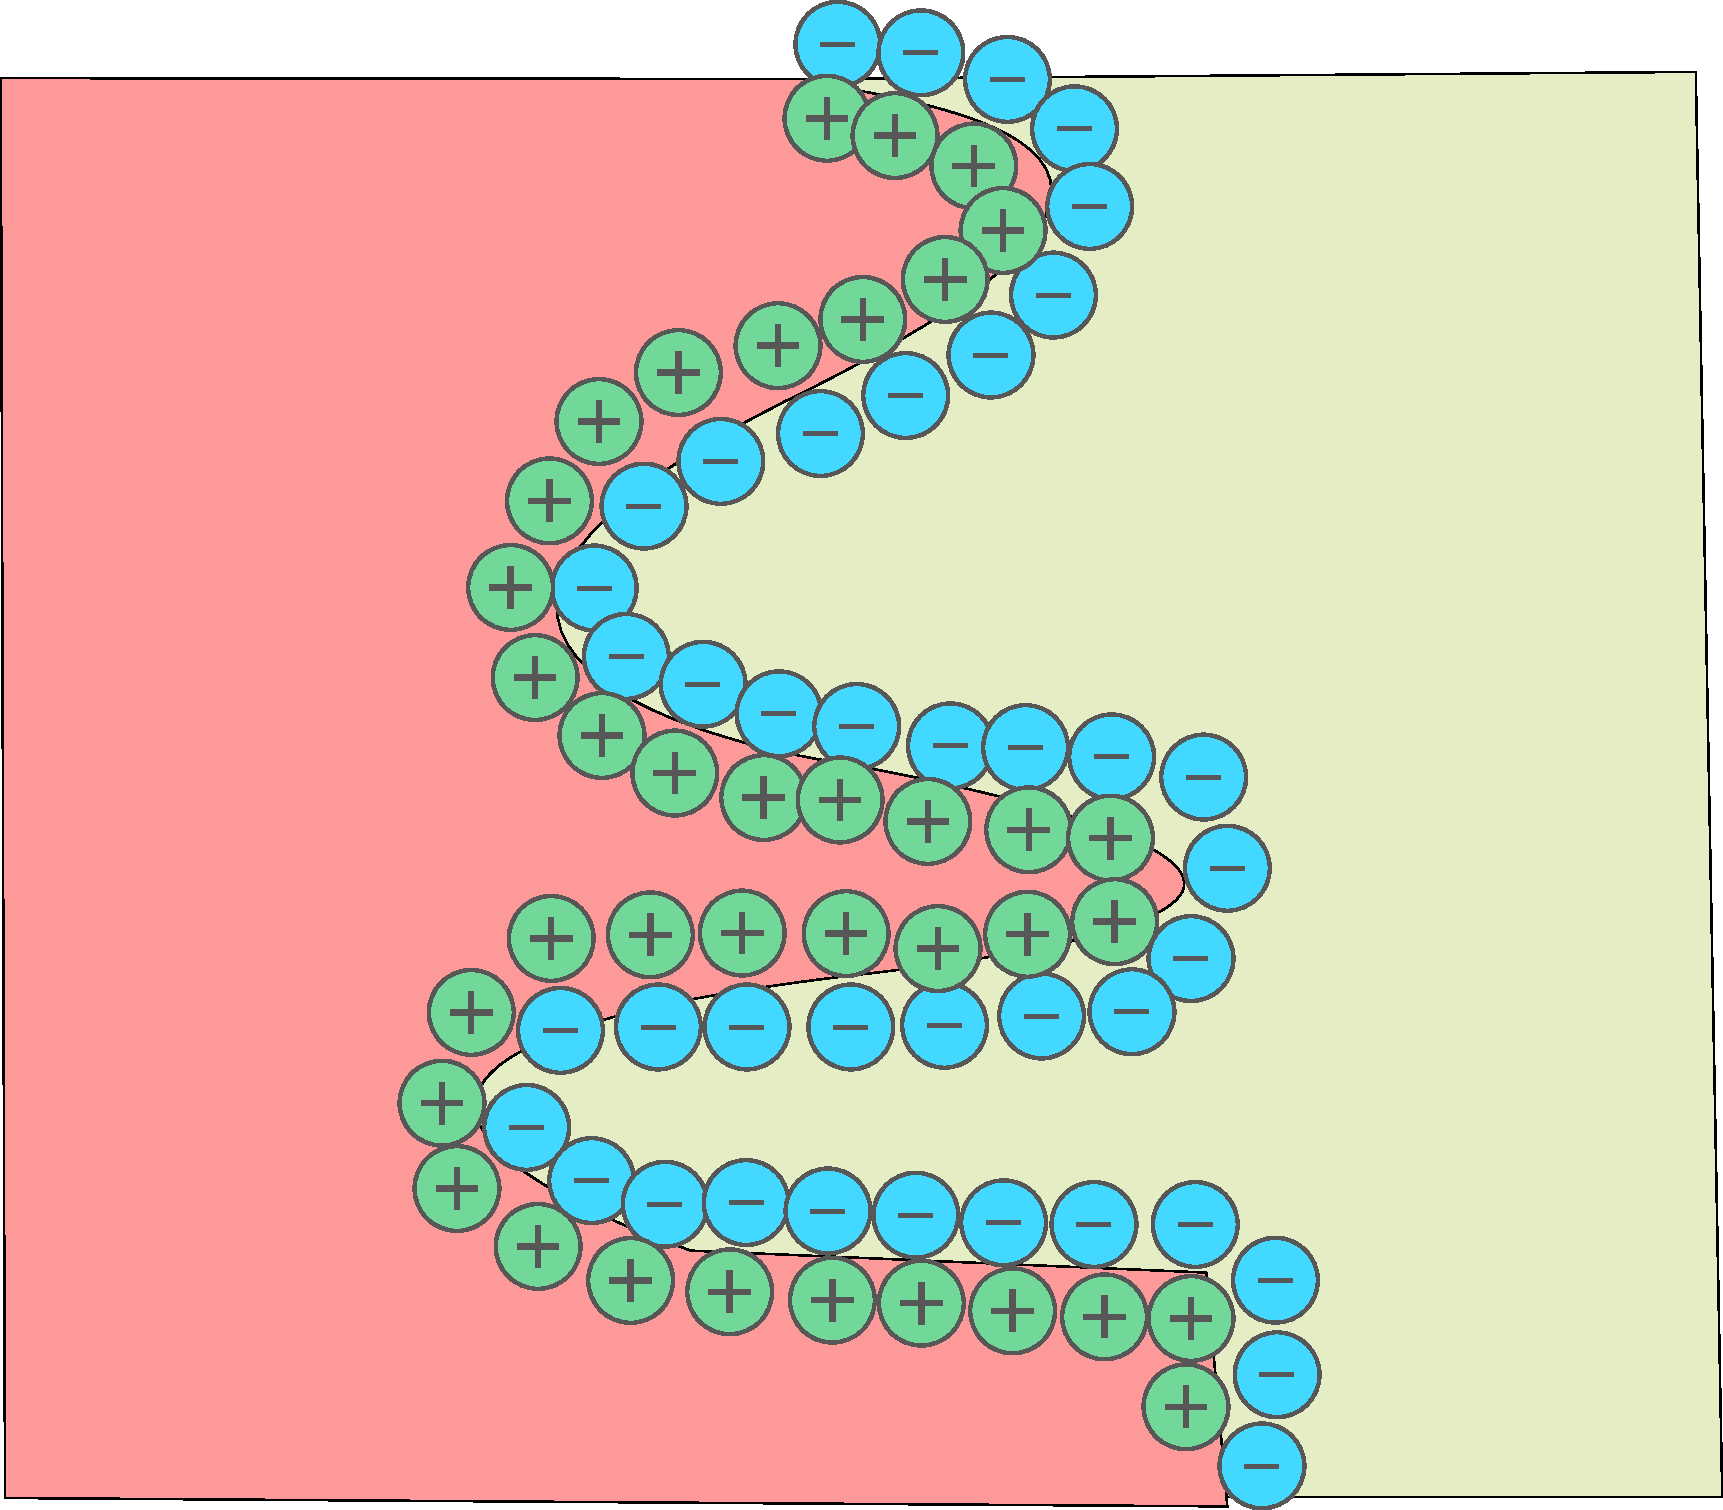
\includegraphics[width=0.75\textwidth]{edlc_zoom.pdf}};
					\end{scope}}
					\end{tikzpicture}
					\caption{Esquema de un supercondensador.}
				\end{figure}
			\end{column}
		\end{columns}
	\end{frame}
		
	\subsection{Nanociencia}
	\begin{frame}{Nanociencia}
		\begin{figure}[h!]
			\centering
			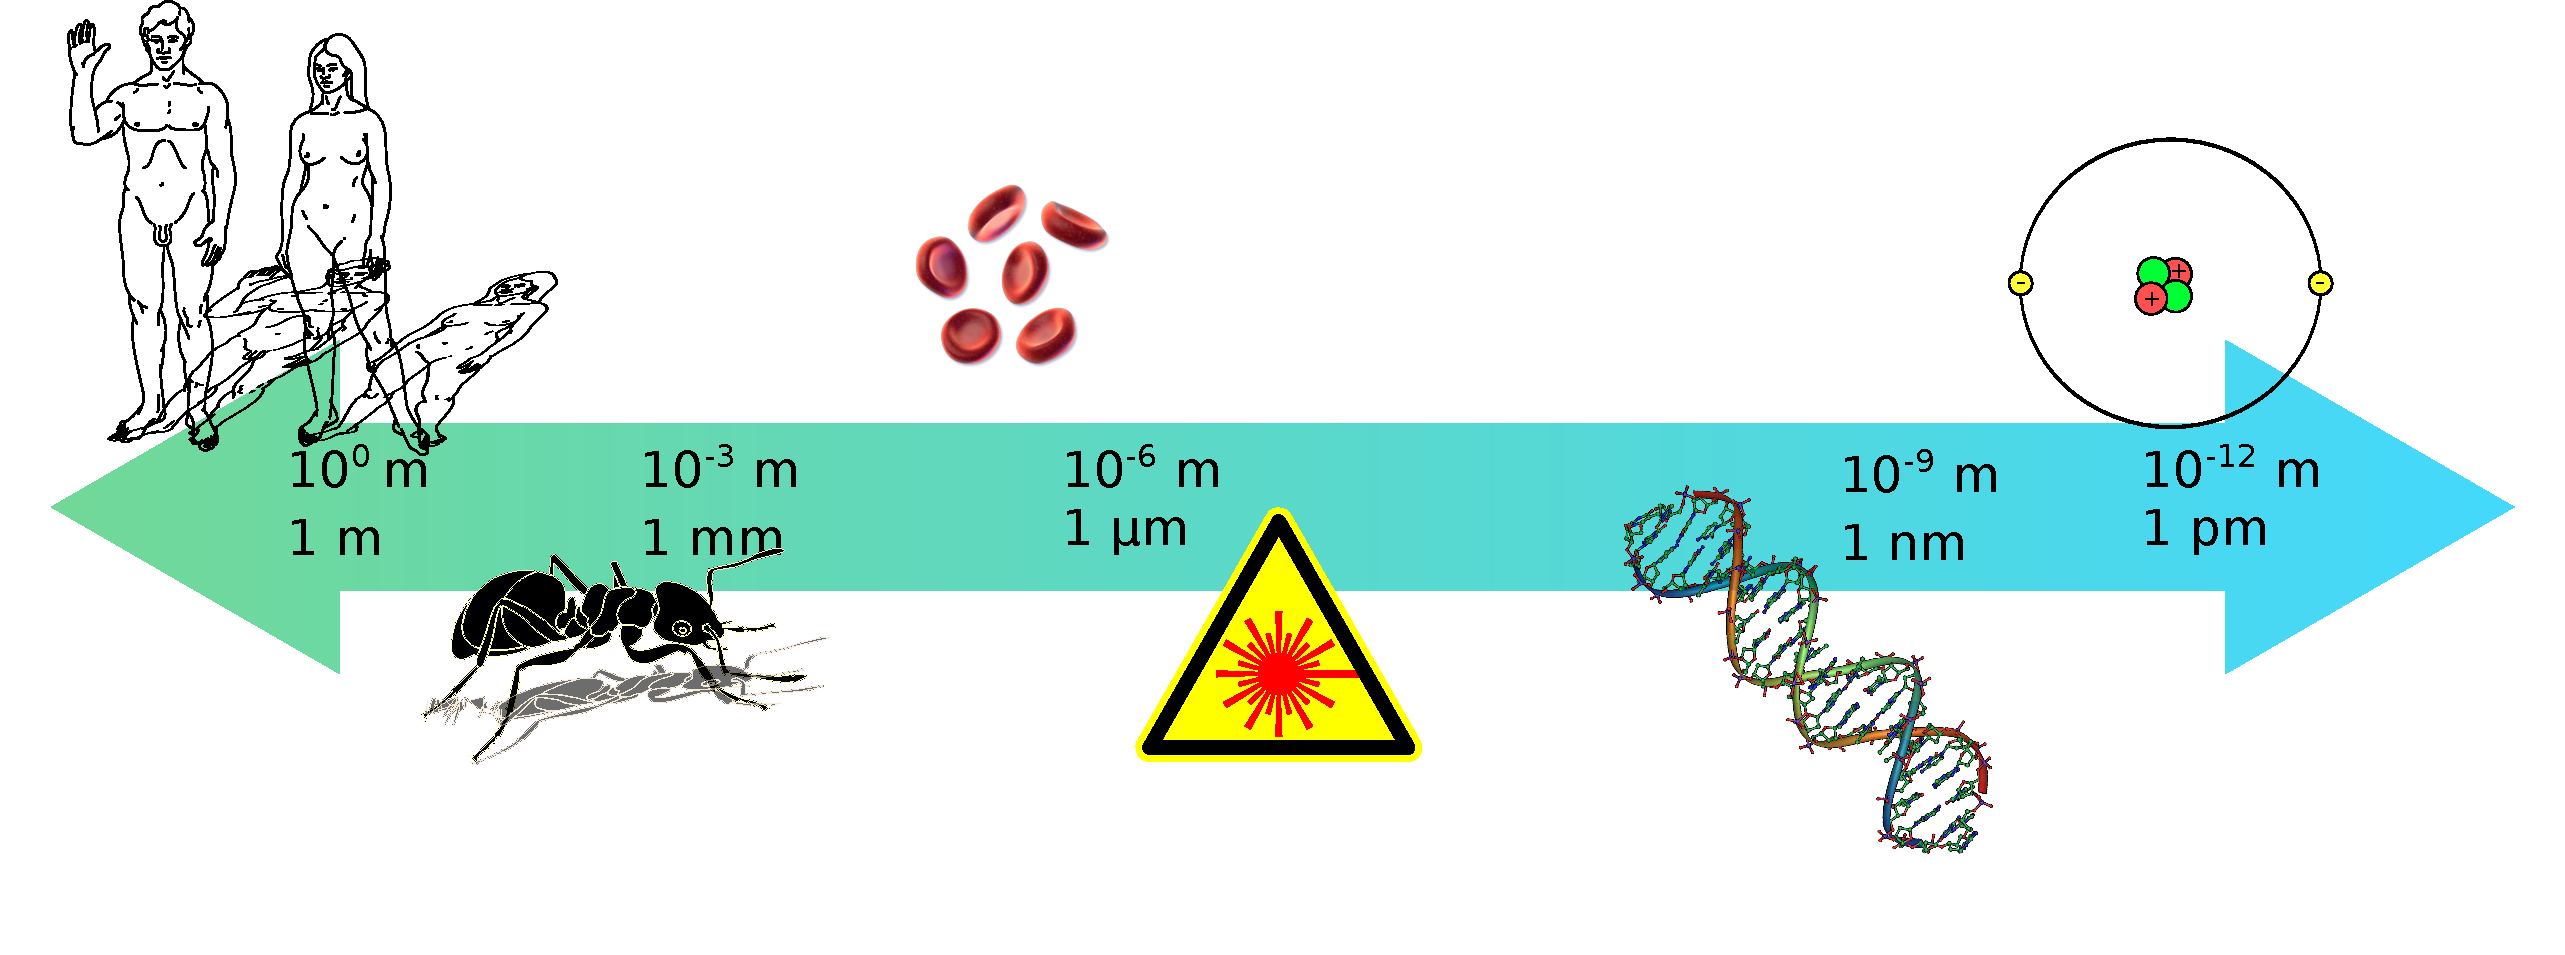
\includegraphics[width=0.9\textwidth]{scale.pdf}
			\caption[Comparativa de ódenes de magnitud desde metros hasta picometros]{Comparativa de órdenes de magnitud. De izquierda a derecha: Escala humana, 1-2 m. Insectos, 10 cm - 1 mm. Glóbulos rojos, 6 $\mathrm{\mu}$m. Longitud de onda de luz visible, 780-380 nm. Transistores en un microprocesador, 100 - 10 nm. Doble hélice de ADN, 2 nm. Radio atómico de un átomo de helio, 31 pm.}
			\label{fig:scale}
		\end{figure}
	\end{frame}

	\begin{frame}{Clasificación de nanomateriales}
		\begin{figure}
			\centering
			\begin{subfigure}[b]{0.15\textwidth}
				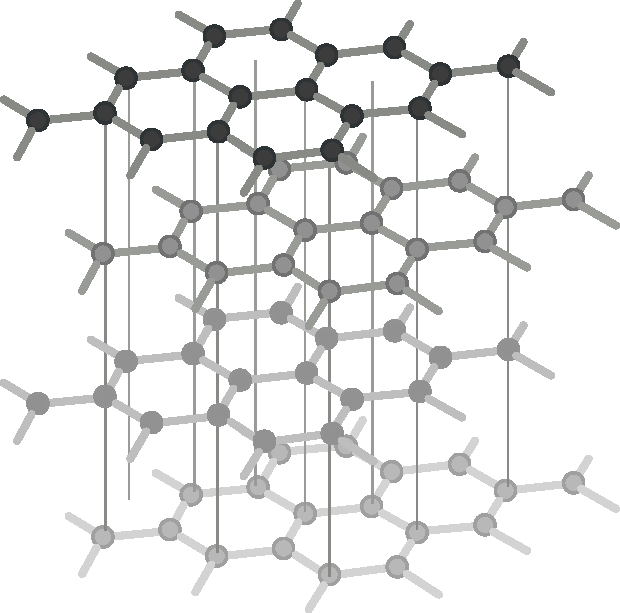
\includegraphics[width=\textwidth]{graphite_structure.pdf}
				\caption{}
				\label{fig:graphite_struct}
			\end{subfigure}
			\begin{subfigure}[b]{0.15\textwidth}
				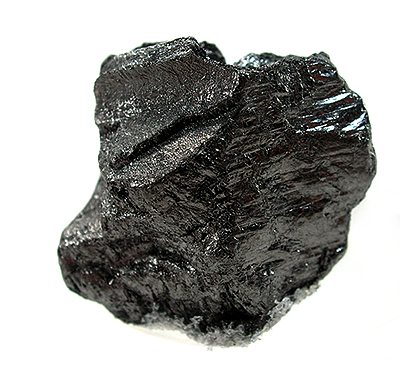
\includegraphics[width=\textwidth]{graphite_image.png}
				\caption{}
				\label{fig:graphite_image}
			\end{subfigure}
			\begin{subfigure}[b]{0.15\textwidth}
				\begin{tikzpicture}
				\node at (0,0) {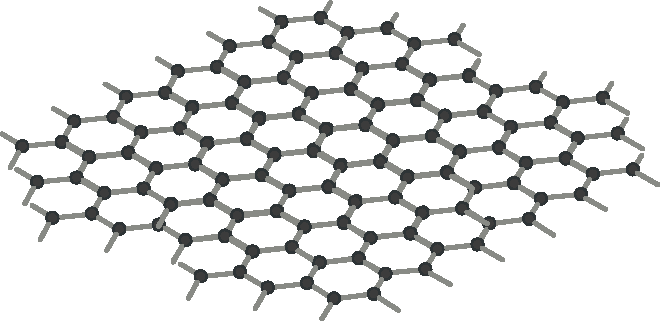
\includegraphics[width=\textwidth]{graphene_structure.pdf}};
%				\only<2>{\draw[red, ultra thick, rounded corners] (-1,-1) rectangle (1,1);}
				\end{tikzpicture}
				\caption{}
				\label{fig:graphene_struct}
			\end{subfigure}
			\begin{subfigure}[b]{0.15\textwidth}
%				\begin{tikzpicture}
%					\node (image) {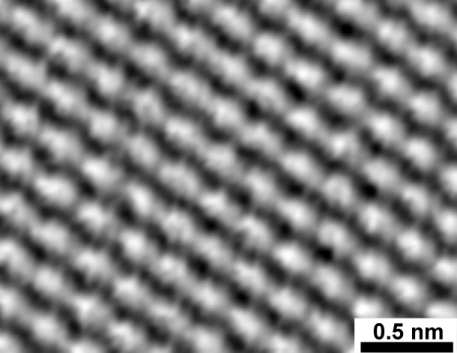
\includegraphics[width=\textwidth]{graphene_image.jpg}};
%				\end{tikzpicture}
				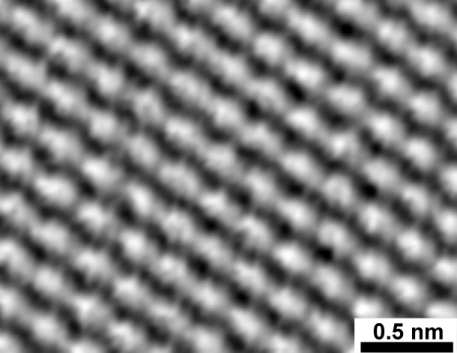
\includegraphics[width=\textwidth]{graphene_image.jpg}
				\caption{}
				\label{fig:graphene_image}
			\end{subfigure}
			\\
			\begin{subfigure}[b]{0.15\textwidth}
				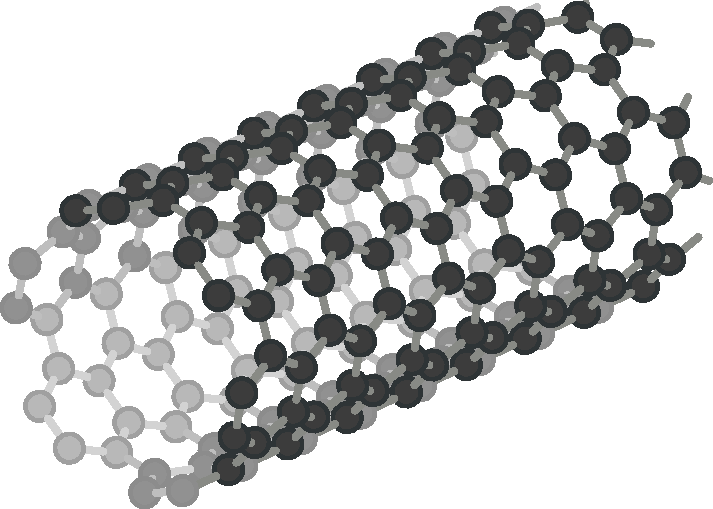
\includegraphics[width=\textwidth]{cnt_structure.pdf}
				\caption{}
				\label{fig:cnt_struct}
			\end{subfigure}
			\begin{subfigure}[b]{0.15\textwidth}
				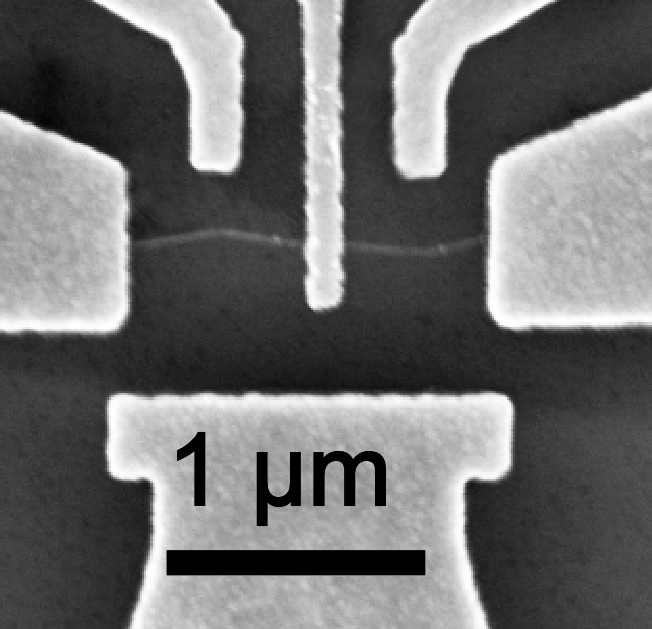
\includegraphics[width=\textwidth]{cnt_image.png}
				\caption{}
				\label{fig:cnt_image}
			\end{subfigure}
			\begin{subfigure}[b]{0.15\textwidth}
				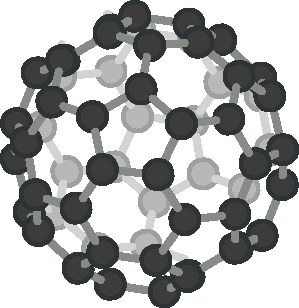
\includegraphics[width=\textwidth]{fullerene_structure.pdf}
				\caption{}
				\label{fig:fullerene_structure}
			\end{subfigure}
			\begin{subfigure}[b]{0.15\textwidth}
				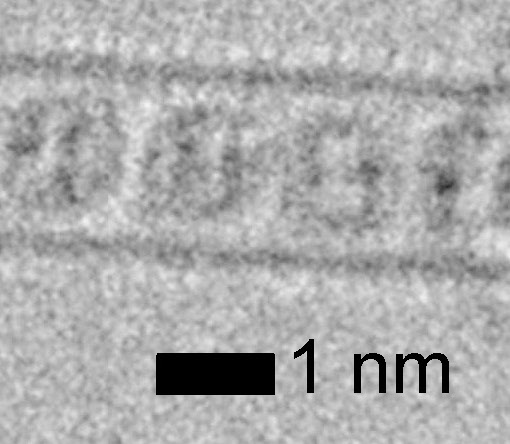
\includegraphics[width=\textwidth]{fullerene_image.jpg}
				\caption{}
				\label{fig:fullerene_image}
			\end{subfigure}
			\caption[Alótropos del carbono mostrando las diferentes dimensionalidades de los nanomateriales]{\subref{fig:graphite_struct} y \subref{fig:graphite_image} grafito natural. \subref{fig:graphene_struct} y \subref{fig:graphene_image} grafeno(Frank Trixler, LMU/CeNS: Organic Semiconductor Group). \subref{fig:cnt_struct} y \subref{fig:cnt_image} nanotubo de carbono, (Pavlos Apostolidis, London Centre for Nanotechnology, Department of Physics \& Astronomy). \subref{fig:fullerene_structure} y \subref{fig:fullerene_image} fullereno\citep{Gimenez2011}.}
			\label{fig:carbon_allotropes}
		\end{figure}
	\end{frame}

	\begin{frame}{Área superficial}
		\begin{figure}
			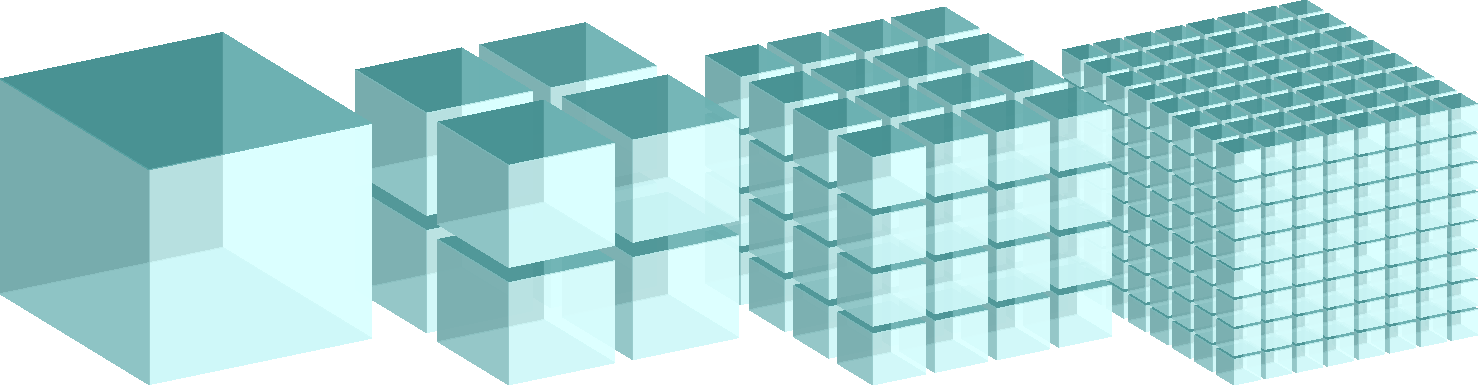
\includegraphics[width=\textwidth]{area_cubes.pdf}
			\caption{Aumento del área superficial.}
		\end{figure}
		\begin{itemize}[<+(1)->]
			\item El \textbf{área superficial se dobla} con cada división.
			\item De 1 cm a 100 nm de lado, \textbf{el área aumenta 100.000 veces}.
		\end{itemize}
	\end{frame}

	\begin{frame}{Grafeno y derivados}
		\begin{columns}
			\begin{column}{0.6\textwidth}
				\only<1->\textbf{¿Qué es el grafeno?}
				\begin{itemize}[<+(1)->]
					\item Red hexagonal de \textbf{átomos de carbono hibridizados}.
					\item Espesor de \textbf{0,34 nm}, con átomos espaciados en \textbf{0,14 nm}.
					\item \textbf{Andre Geim y Konstantin Novoselov} recibieron el premio Nobel en 2010 por aislar grafeno \citep{Novoselov2004}.
				\end{itemize}
			\end{column}
			\begin{column}{0.4\textwidth}
				\begin{onlyenv}<1-3>
					\begin{figure}
						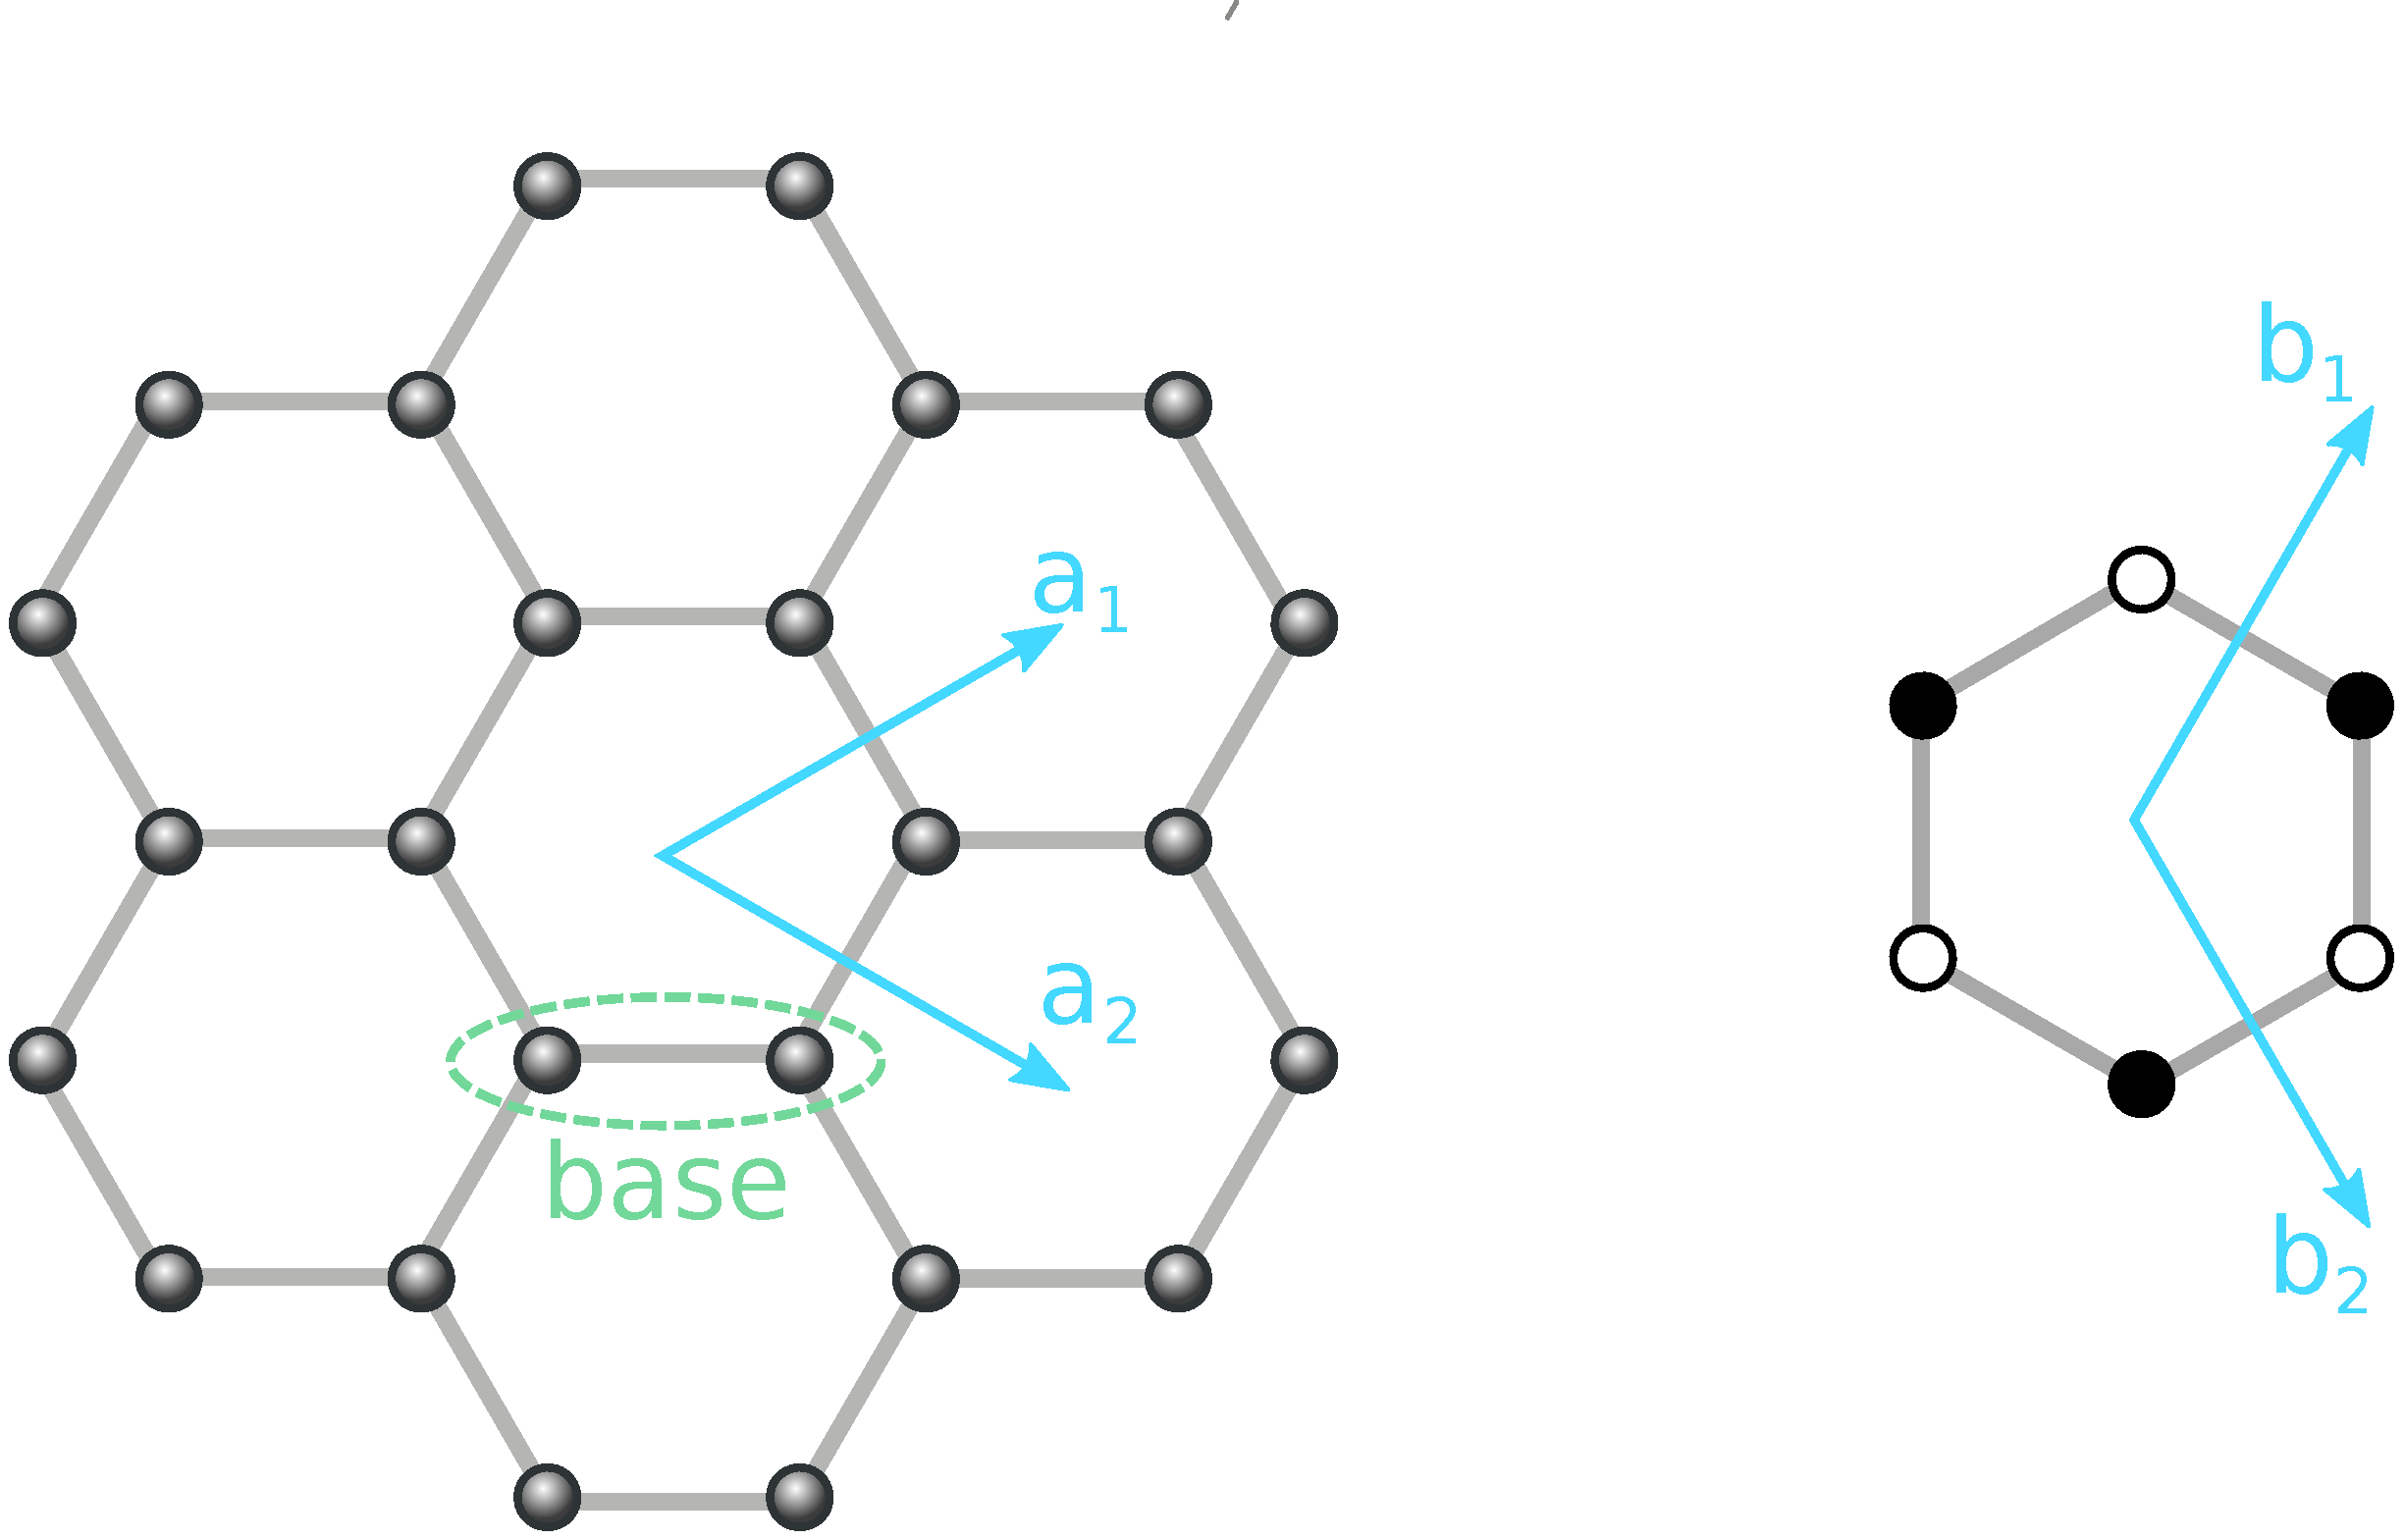
\includegraphics[width=\textwidth]{graphene_lattice.pdf}
						\caption{Estructura cristalina del grafeno.}
					\end{figure}
				\end{onlyenv}
				\begin{onlyenv}<4->
					\begin{figure}
						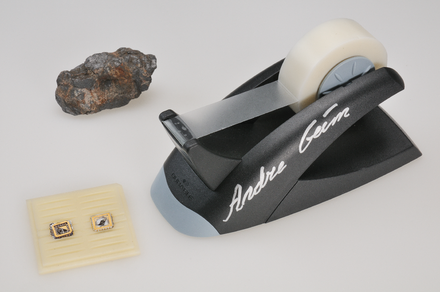
\includegraphics[width=\textwidth]{Nobel_graphene.png}
						\caption{Método experimental para la obtención de grafeno \citep{Novoselov2004}.}
					\end{figure}
				\end{onlyenv}
			\end{column}
		\end{columns}
	\end{frame}

	\begin{frame}{Grafeno y derivados}
		\begin{columns}
			\begin{column}{0.6\textwidth}
				\only<1->\textbf{Derivados del grafeno}
				\begin{itemize}[<+(1)->]
					\item Una forma de producir grafeno en grandes cantidades en mediante la \textbf{ruta del óxido de grafeno}.
					\item La introducción de \textcolor{red_oxigen}{\textbf{grupos oxigenados}} en el grafito, facilita la \textbf{exfoliación} de \textbf{óxido de grafeno (GO)}.
					\item La remoción de los \textcolor{red_oxigen}{\textbf{grupos oxigenados}} resulta en \textbf{óxido de grafeno reducido (rGO)}.
					\item[] \textcolor{red}{\textbf{Lamentablemente este método no es perfecto}}.
				\end{itemize}
			\end{column}
			\begin{column}{0.4\textwidth}
				\begin{onlyenv}<1->
					\begin{figure}
						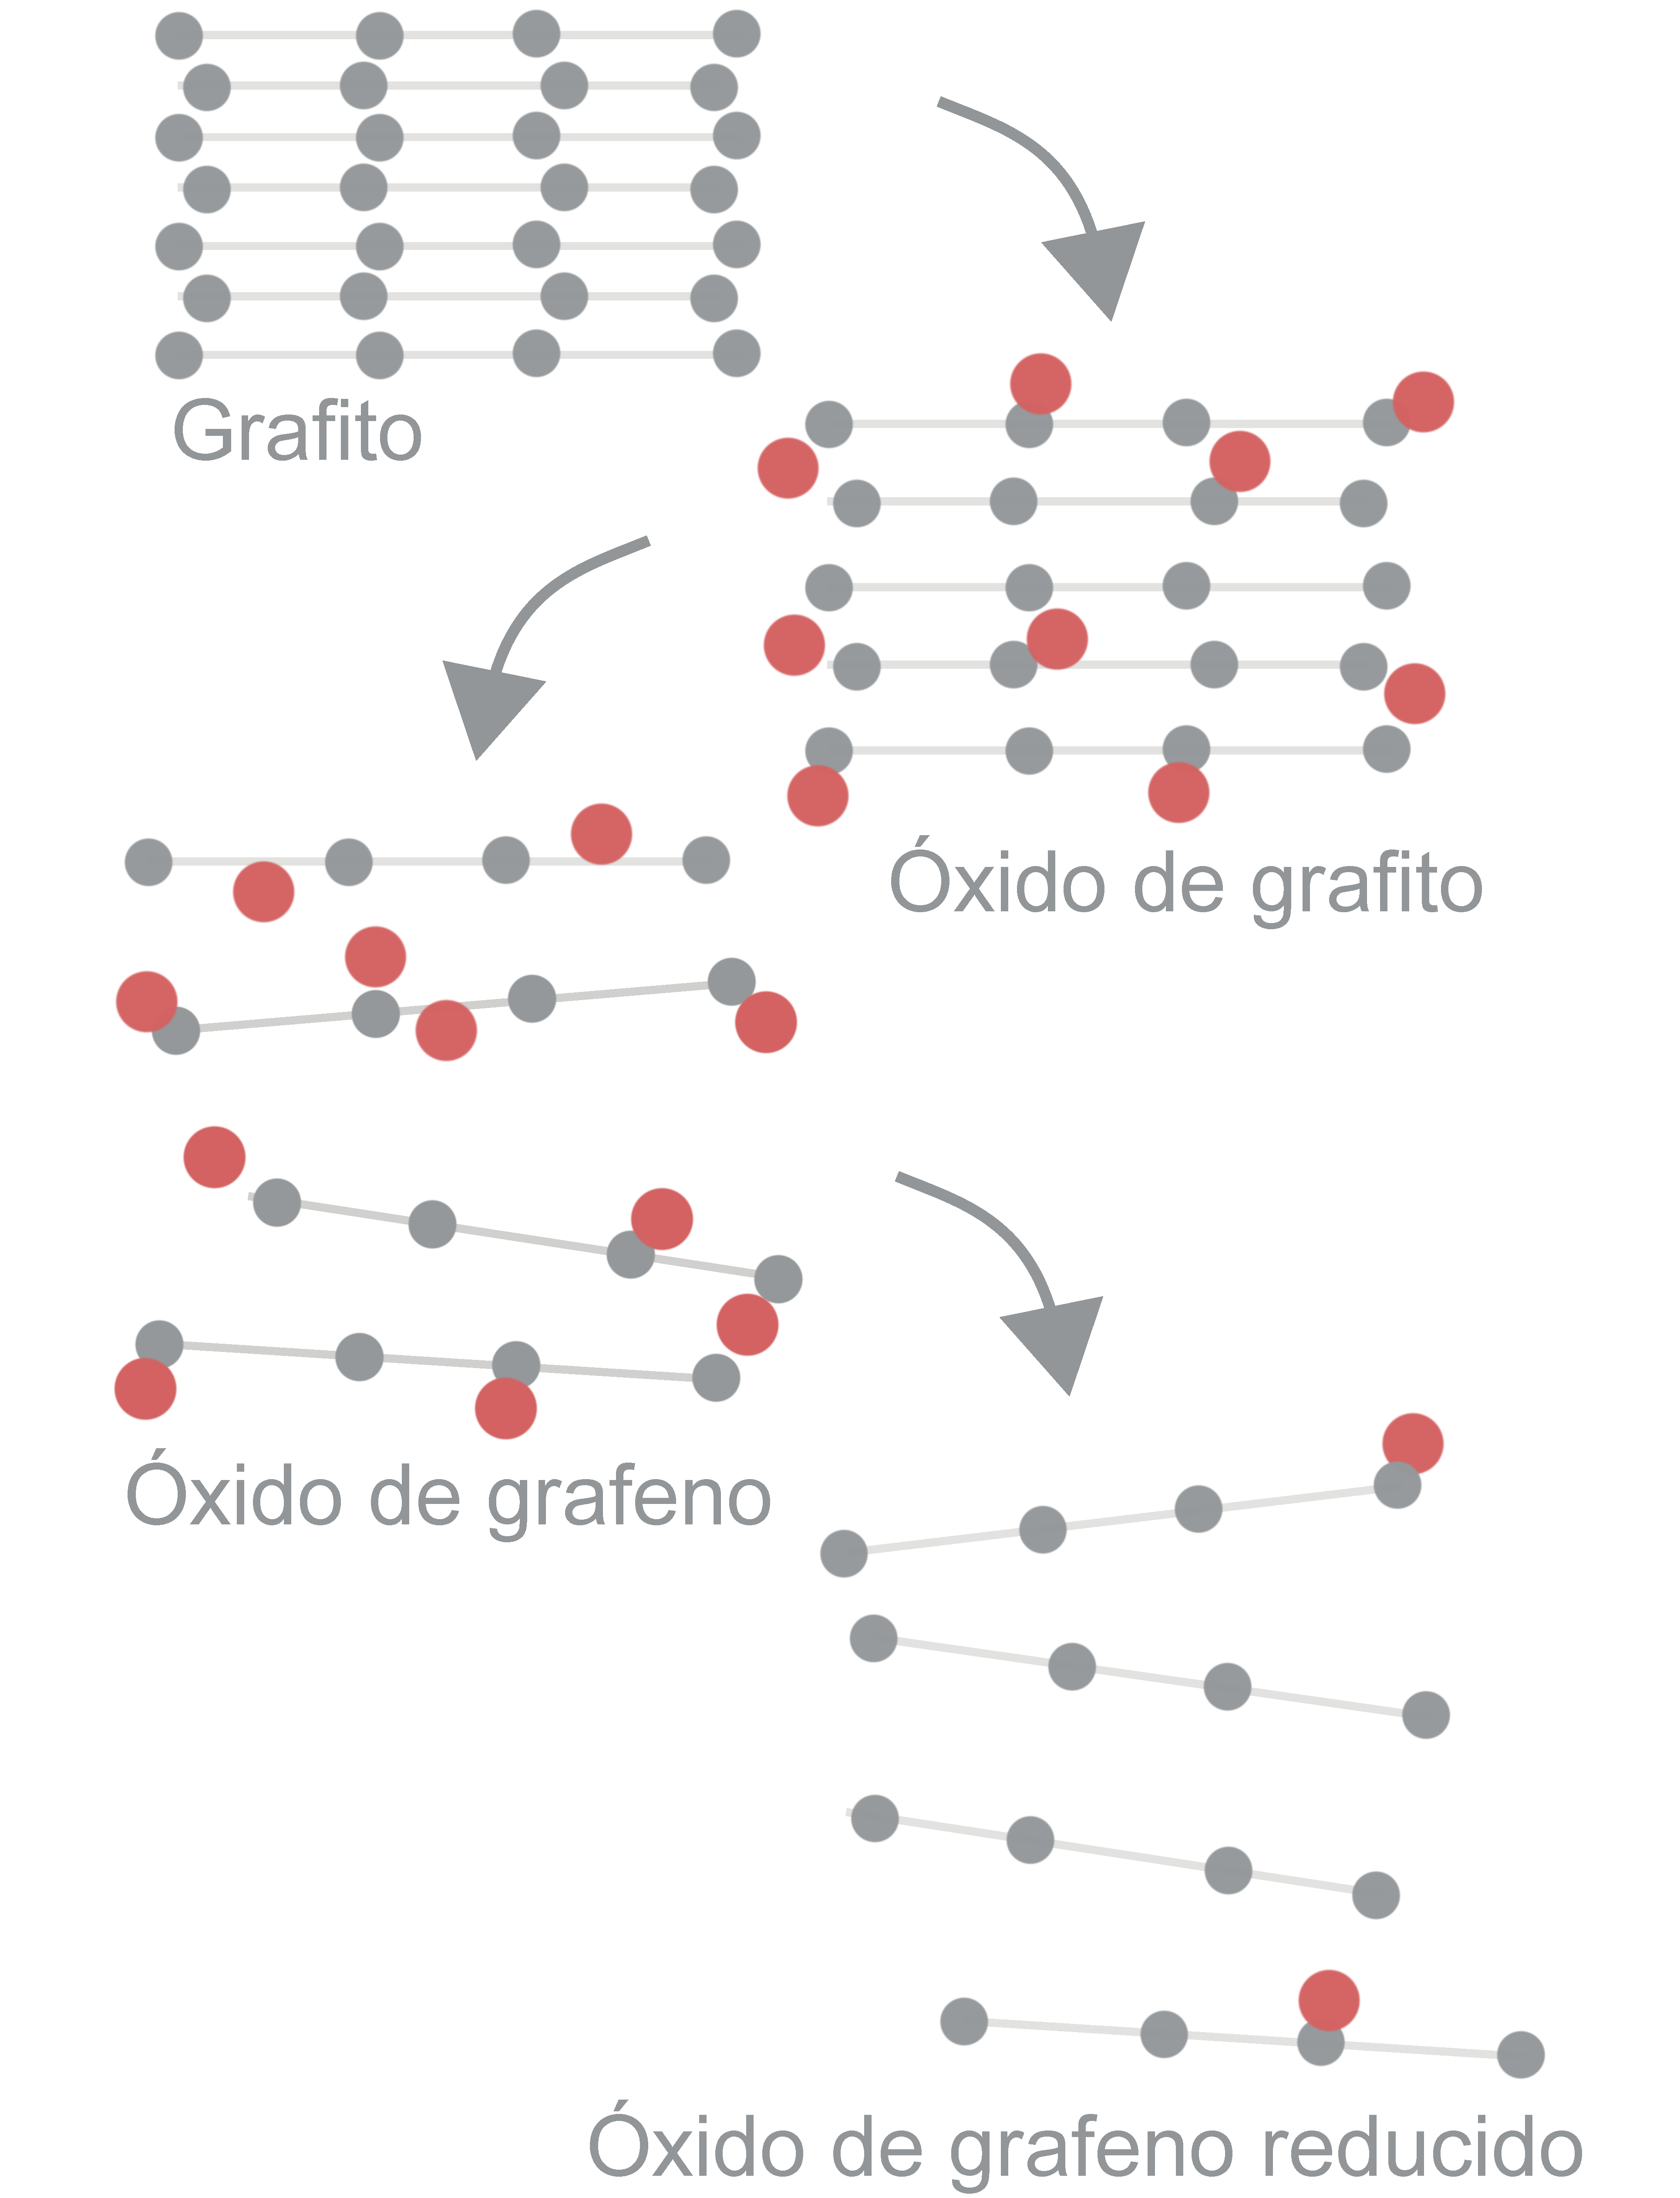
\includegraphics[width=0.8\textwidth]{graphiteToRGO_stack.pdf}
						\caption{Ruta del óxido de grafeno.}
					\end{figure}
				\end{onlyenv}
			\end{column}
		\end{columns}
	\end{frame}

	\begin{frame}{El grafeno en supercondensadores}
		\only<1->\textbf{¿Por qué usar grafeno en supercondensadores?}
		\begin{itemize}[<+(1)->]
			\item Es un material \textbf{no metálico} con \textbf{alta conductividad eléctrica}.
			\item Tiene un \textbf{área superficial específica} muy grande. Un gramo de grafeno tiene el área aproximada a 14 canchas de tenis.
			\item Un gramo de \textbf{óxido reducido de grafeno} puede llegar a aproximadamente 3.
		\end{itemize}
	\end{frame}


	\subsection{Caracterización electroquímica}
	
	\begin{frame}[fragile]{Caracterización de supercondensadores}
		\begin{columns}
			\begin{column}{0.5\textwidth}
				\only<1-> \textbf{Voltametría cíclica}
				\begin{itemize}[<+(1)->]
					\item \textbf{Barrido de voltaje a velocidad constante}, y medición de \textbf{corriente}.
					\item El área encerrada es \textbf{proporcional a la capacitancia específica}.
					\item Un \textbf{condensador ideal} mostraría un rectángulo.
				\end{itemize}
			\end{column}
			\begin{column}{0.5\textwidth}
				\begin{figure}
					\begin{tikzpicture}
					[scale=1,trim axis right,trim axis left]
						\begin{axis}
						[
						CVStyle,
						width=\textwidth,
						domain=-1:1,
						legend entries={Ideal, Real},				
						]
							\addplot[green!60!black, thick] table {
								A B
								-1  1
								1  1
								
								1 -1
								-1 -1
							};
							\addplot[green!60!black, thick, dashed, forget plot] table {
								A B
								-1 -1
								-1  1
								
								1  1
								1 -1
							};
							\addplot[thick,color=red, smooth,samples=100,domain=0:0.4] plot[parametric] function{1.57041*t**(3)+0*t**(2)+0.4621*t-1,-0.11402*t**(3)+0*t**(2)+3.25798*t-1};
							\addplot[thick,color=red, smooth,samples=100,domain=0.4:0.54] plot[parametric] function{8.70966*t**(3)-8.49528*t**(2)+3.83173*t-1.44552,-14.95269*t**(3)+17.65714*t**(2)-3.74567*t-0.07401};
							\addplot[thick,color=red, smooth,samples=100,domain=0.54:0.8] plot[parametric] function{-8.63754*t**(3)+19.61633*t**(2)-11.35349*t+1.28871,7.29314*t**(3)-18.39283*t**(2)+15.72766*t-3.58035};
							\addplot[thick,color=red, smooth,samples=100,domain=0.80:1.0] plot[parametric] function{1.73159*t**(3)-5.19477*t**(2)+8.43573*t-3.97255,1.55121*t**(3)-4.65363*t**(2)+4.76933*t-0.66691};
							
							\addplot[thick, red, smooth, samples=100,domain=0:0.4] plot[parametric] function{-1.57041*t**(3)+0*t**(2)-0.4621*t+1,0.11402*t**(3)+0*t**(2)-3.25798*t+1};
							\addplot[thick, red, smooth, samples=100,domain=0.4:0.54] plot[parametric] function{-8.70966*t**(3)+8.49528*t**(2)-3.83173*t+1.44552,14.95269*t**(3)-17.65714*t**(2)+3.74567*t+0.07401};
							\addplot[thick, red, smooth, samples=100,domain=0.54:0.8] plot[parametric] function{8.63754*t**(3)-19.61633*t**(2)+11.35349*t-1.28871,-7.29314*t**(3)+18.39283*t**(2)-15.72766*t+3.58035};
							\addplot[thick, red, smooth, samples=100,domain=0.80:1.0] plot[parametric] function{-1.73159*t**(3)+5.19477*t**(2)-8.43573*t+3.97255,-1.55121*t**(3)+4.65363*t**(2)-4.76933*t+0.66691};
						\end{axis}
					\end{tikzpicture}
					\caption{Ejemplos de voltametría cíclica.}
				\end{figure}
			\end{column}
		\end{columns}
	\end{frame}
	
	\newcommand{\circuitscale}{0.5}	
	\begin{frame}[fragile]{Caracterización de supercondensadores}
		\begin{columns}
			\begin{column}{0.5\textwidth}
				\only<1-> \textbf{Espectroscopia de impedancia electroquímica}
				\begin{onlyenv}<1-5>
					\begin{itemize}[<+(1)->]
						\item \textbf{Barrido en frecuencia} de una señal sinusoidal.
						\item Medición de la \textbf{impedancia} en función de la frecuencia.
						\item Representación en un \textbf{gráfico de Nyquist}.
						\item Cualitativamente podemos asignar un \textbf{circuito equivalente} al dispositivo en cuestión.
					\end{itemize}
				\end{onlyenv}
					\begin{onlyenv}<6>
						\begin{figure}[h!]
							\centering
							\begin{subfigure}[b]{0.5\textwidth}
								\begin{circuitikz}[scale = \circuitscale, transform shape, font=\large]
									\draw (0,0)
									to [R=$R_s$,  o-] (2,0)
									to [short] (2,-1)
									to [C=$C_{dl}$] (4,-1)
									to [short] (4,0)
									(2,0) to [short] (2,1)
									to [R=$R_{leak}$] (4,1)
									to [short] (4,0)
									to [short, -o] (5,0);
								\end{circuitikz}
								\caption{Circuito equivalente clásico.}
								\label{fig:eq_classic}
							\end{subfigure}\hfill
							\begin{subfigure}[b]{0.5\textwidth}
								\begin{circuitikz}[scale = \circuitscale, transform shape, font=\large]
									\draw (0,0)
									to [R=$R_s$,  o-] (2,0)
									to [short] (2,-1)
									to [R=$R$] (4,-1)
									to [twoport, t=$W$] (6,-1)
									to [short] (6,0)
									(2,0) to [short] (2,1)
									to [C=$C_{dl}$] (6,1)
									to [short] (6,0)
									to [short, -o] (7,0);
								\end{circuitikz}
								\caption{Circuito equivalente Randles.}
								\label{fig:eq_randles}
							\end{subfigure}
							\caption[Circuitos equivalentes]{Circuitos equivalentes.}
							\label{fig:ciruitos_equivalente}
						\end{figure}	
					\end{onlyenv}
			\end{column}
			\begin{column}{0.5\textwidth}
				\begin{figure}
					\centering
					\begin{tikzpicture}[scale=\plotscale,trim axis right,trim axis left]
						\begin{axis}[
						width=1.3\textwidth,
						height=\axisdefaultheight,
						EISStyle,
						every axis legend/.append style={
							font=\normalsize,
							at={(0.02,0.98)},
							anchor=north west,
						},
						legend entries = {Circuito equivalente clásico, Circuito equivalente Randles}
						]
						\pgfplotstableread{./Data/eisgalv_sim_simple.txt}{\eistable};
						\pgfplotstablegetrowsof{\eistable}
						\pgfmathsetmacro{\N}{\pgfplotsretval}
						\addplot table [only marks, x=Zreal, y expr=\thisrow{Zimag}] {\eistable}
						node[pos=(1-1)/(\N-1), pin=right:{1 MHz}]{}
						node[pos=(\N-1)/(\N-1), pin=right:{0,1 Hz}]{};
						\pgfplotstableread{./Data/eisgalv_sim_warburg.txt}{\eistable};
						\pgfplotstablegetrowsof{\eistable}
						\pgfmathsetmacro{\N}{\pgfplotsretval}
						\addplot table [only marks, x=Zreal, y expr=\thisrow{Zimag}] {\eistable}
						node[pos=(1-1)/(\N-1), pin=left:{1 MHz}]{}
						node[pos=(\N-1)/(\N-1), pin=left:{0,1 Hz}]{};
						\end{axis}
					\end{tikzpicture}
					\caption{Espectro electroquímico de impedancia simulados para los circuitos equivalentes. Obtenido en EIS Spectrum Analyser.}
				\end{figure}
			\end{column}
		\end{columns}
	\end{frame}
	

	\begin{frame}[fragile]{Caracterización de supercondensadores}
		\begin{columns}
			\begin{column}{0.5\textwidth}
				\only<1-> \textbf{Carga y descarga cíclica a corriente constante}
				\begin{itemize}[<+(1)->]
					\item Carga a \textbf{corriente constante} hasta un \textbf{potencial máximo}.
					\item Descarga a \textbf{corriente constante} hasta un \textbf{potencial mínimo}.
					\item Se evidencia el efecto de la\textbf{ resistencia en serie equivalente} como una \textbf{caída de potencial}.
				\end{itemize}
			\end{column}
			\begin{column}{0.5\textwidth}
				\begin{figure}
					\begin{tikzpicture}
					[scale=1,trim axis right,trim axis left]
						\begin{axis}
						[
						CCDStyle,
						width=\textwidth,
						legend entries={Ideal, Real}			
						]
						\addplot[green!60!black, thick] table {
							A B
							0 0
							1 1
							2 0
						};
						\addplot[red, thick, domain=0:1] (\x,{-0.8*(\x)^(2)+1.6*(\x)+0.2});
						\addplot[red, thick, domain=1:2] (\x,{0.8*(\x)^(2)-3.2*(\x)+3.2});
						\addplot[red, thick, dashed] table {
							A B
							0 0
							0 0.2
							
							1 1
							1 0.8
						};
						\draw [arrows={|-|}] (axis cs:1.1,1) -- node[right]{$iR$} (axis cs:1.1,0.8);
						\draw [arrows={|-|}] (axis cs:0.1,0.2) -- node[right]{$iR$} (axis cs:0.1,0);
						\end{axis}
					\end{tikzpicture}
					\caption{Ejemplo de carga y descarga.}
				\end{figure}			
			\end{column}
		\end{columns}
	\end{frame}
	

	\newcommand{\clipradius}{1.7cm}
	\section{Ruta de síntesis}
	\begin{frame}{Ruta de síntesis}
%		\begin{figure}
%			\centering
%			\fbox{
%				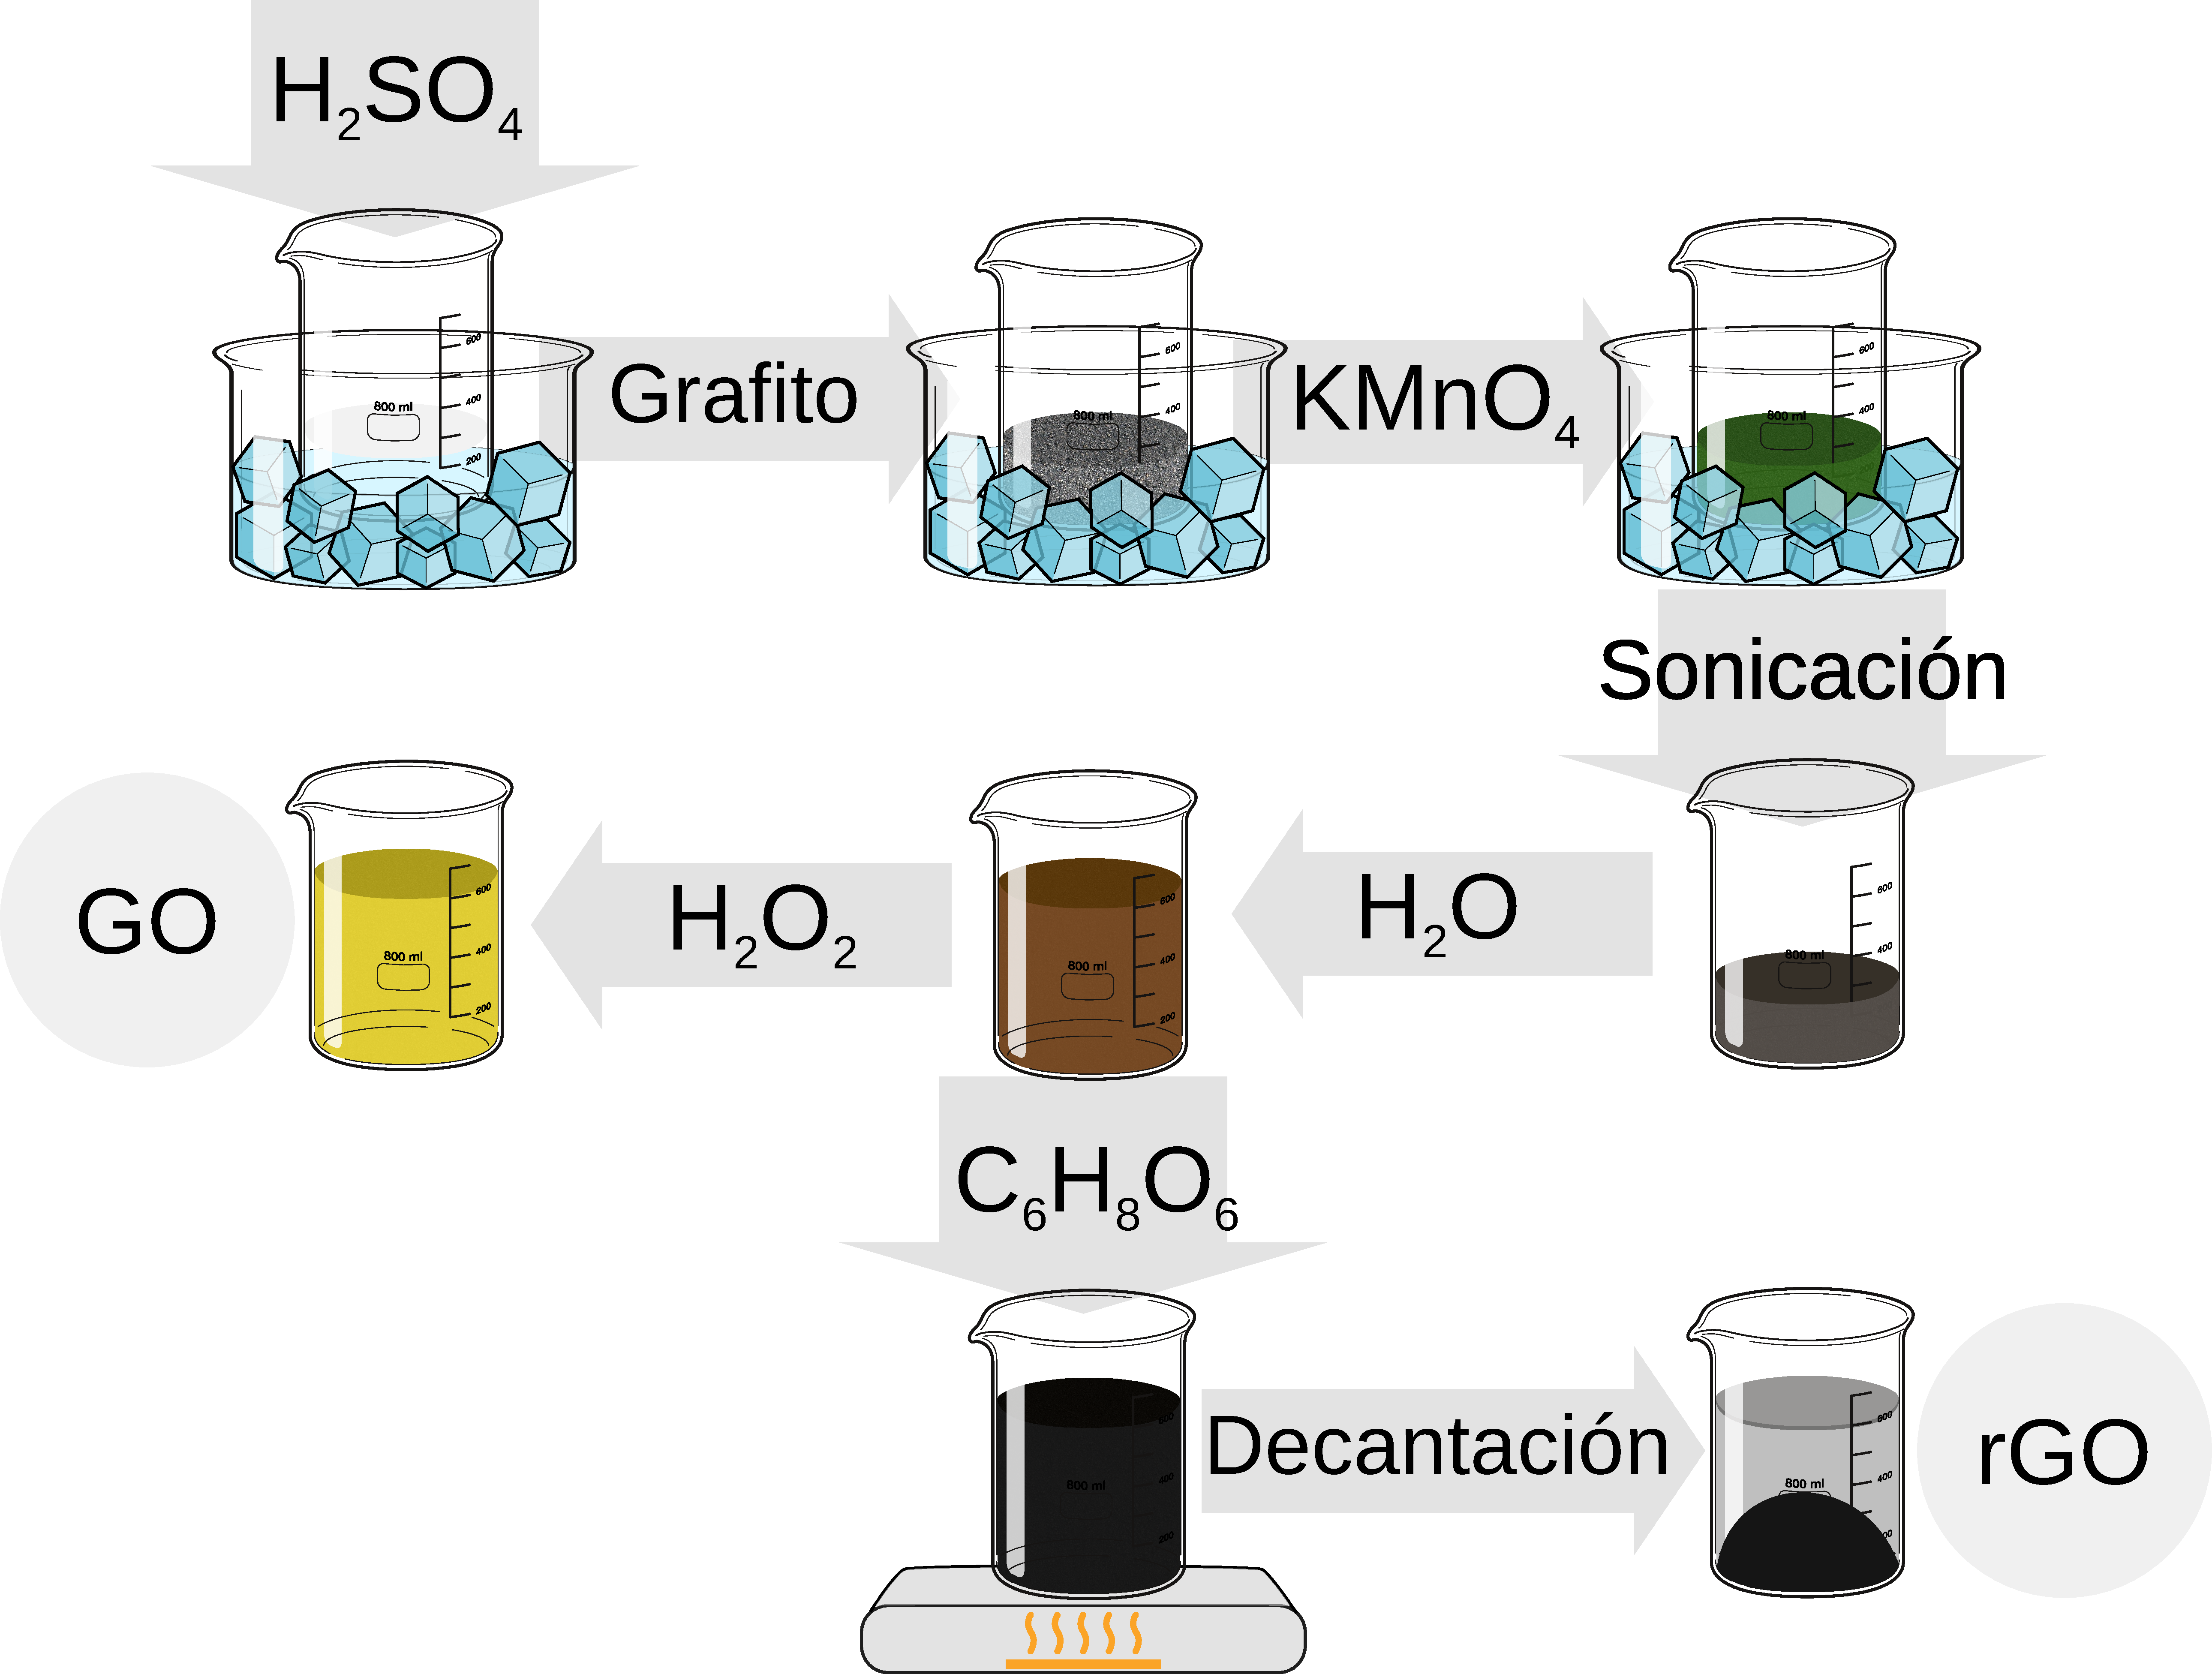
\includegraphics[width=0.8\textwidth]{experimental_method.pdf}
%			}
%			\caption[Método experimental simplicado para la síntesis de óxido de grafeno y óxido reduxido de grafeno]{Método experimental simplificado para la síntesis de óxido de grafeno y óxido reducido de grafeno.}
%		\end{figure}
		\begin{figure}
			\begin{tikzpicture}[]
			\path[ use as bounding box] (-4,-2) rectangle (4,2);
%			\draw [help lines, dashed] (-4,-2) grid (4,2);
				\only<1->{\begin{scope}
					\clip[] (-5, 1)	rectangle (-2.2, 4);
					\node at (0, 0) {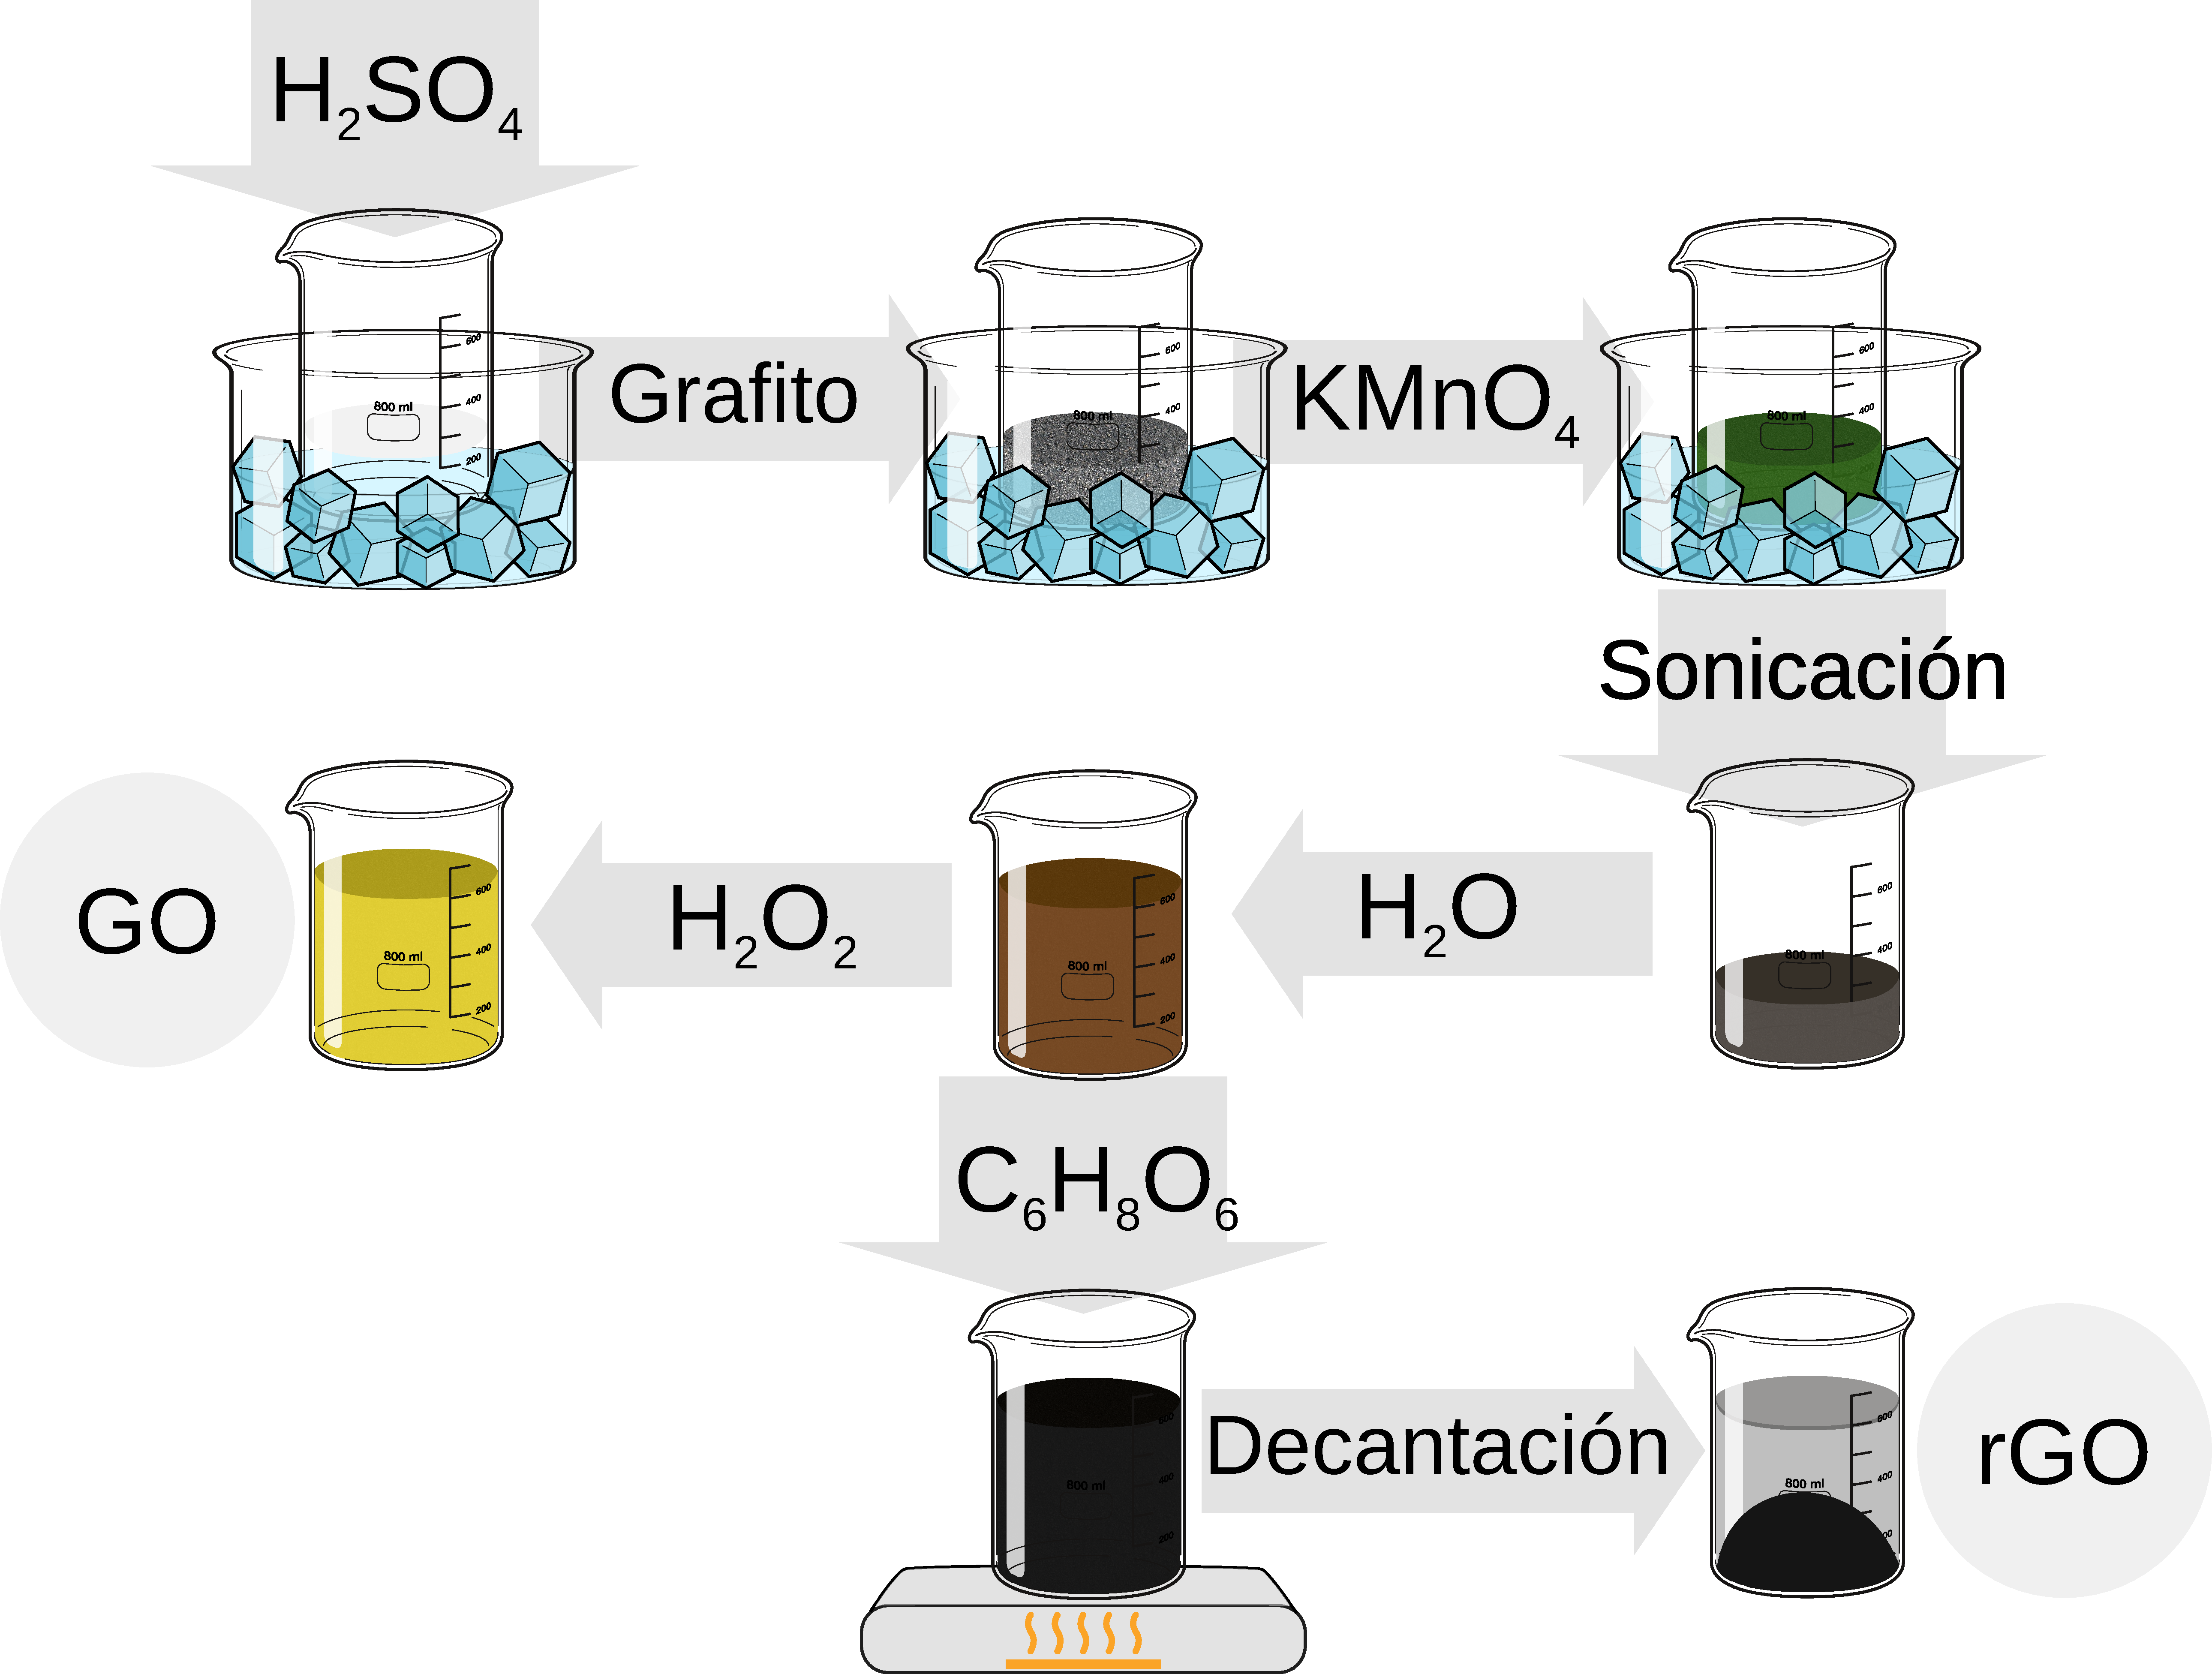
\includegraphics[width=0.7\textwidth]{experimental_method.pdf}};
				\end{scope}}
				\only<2->{\begin{scope}
					\clip[] (-2.2, 1) rectangle (1, 4);
					\node at (0, 0) {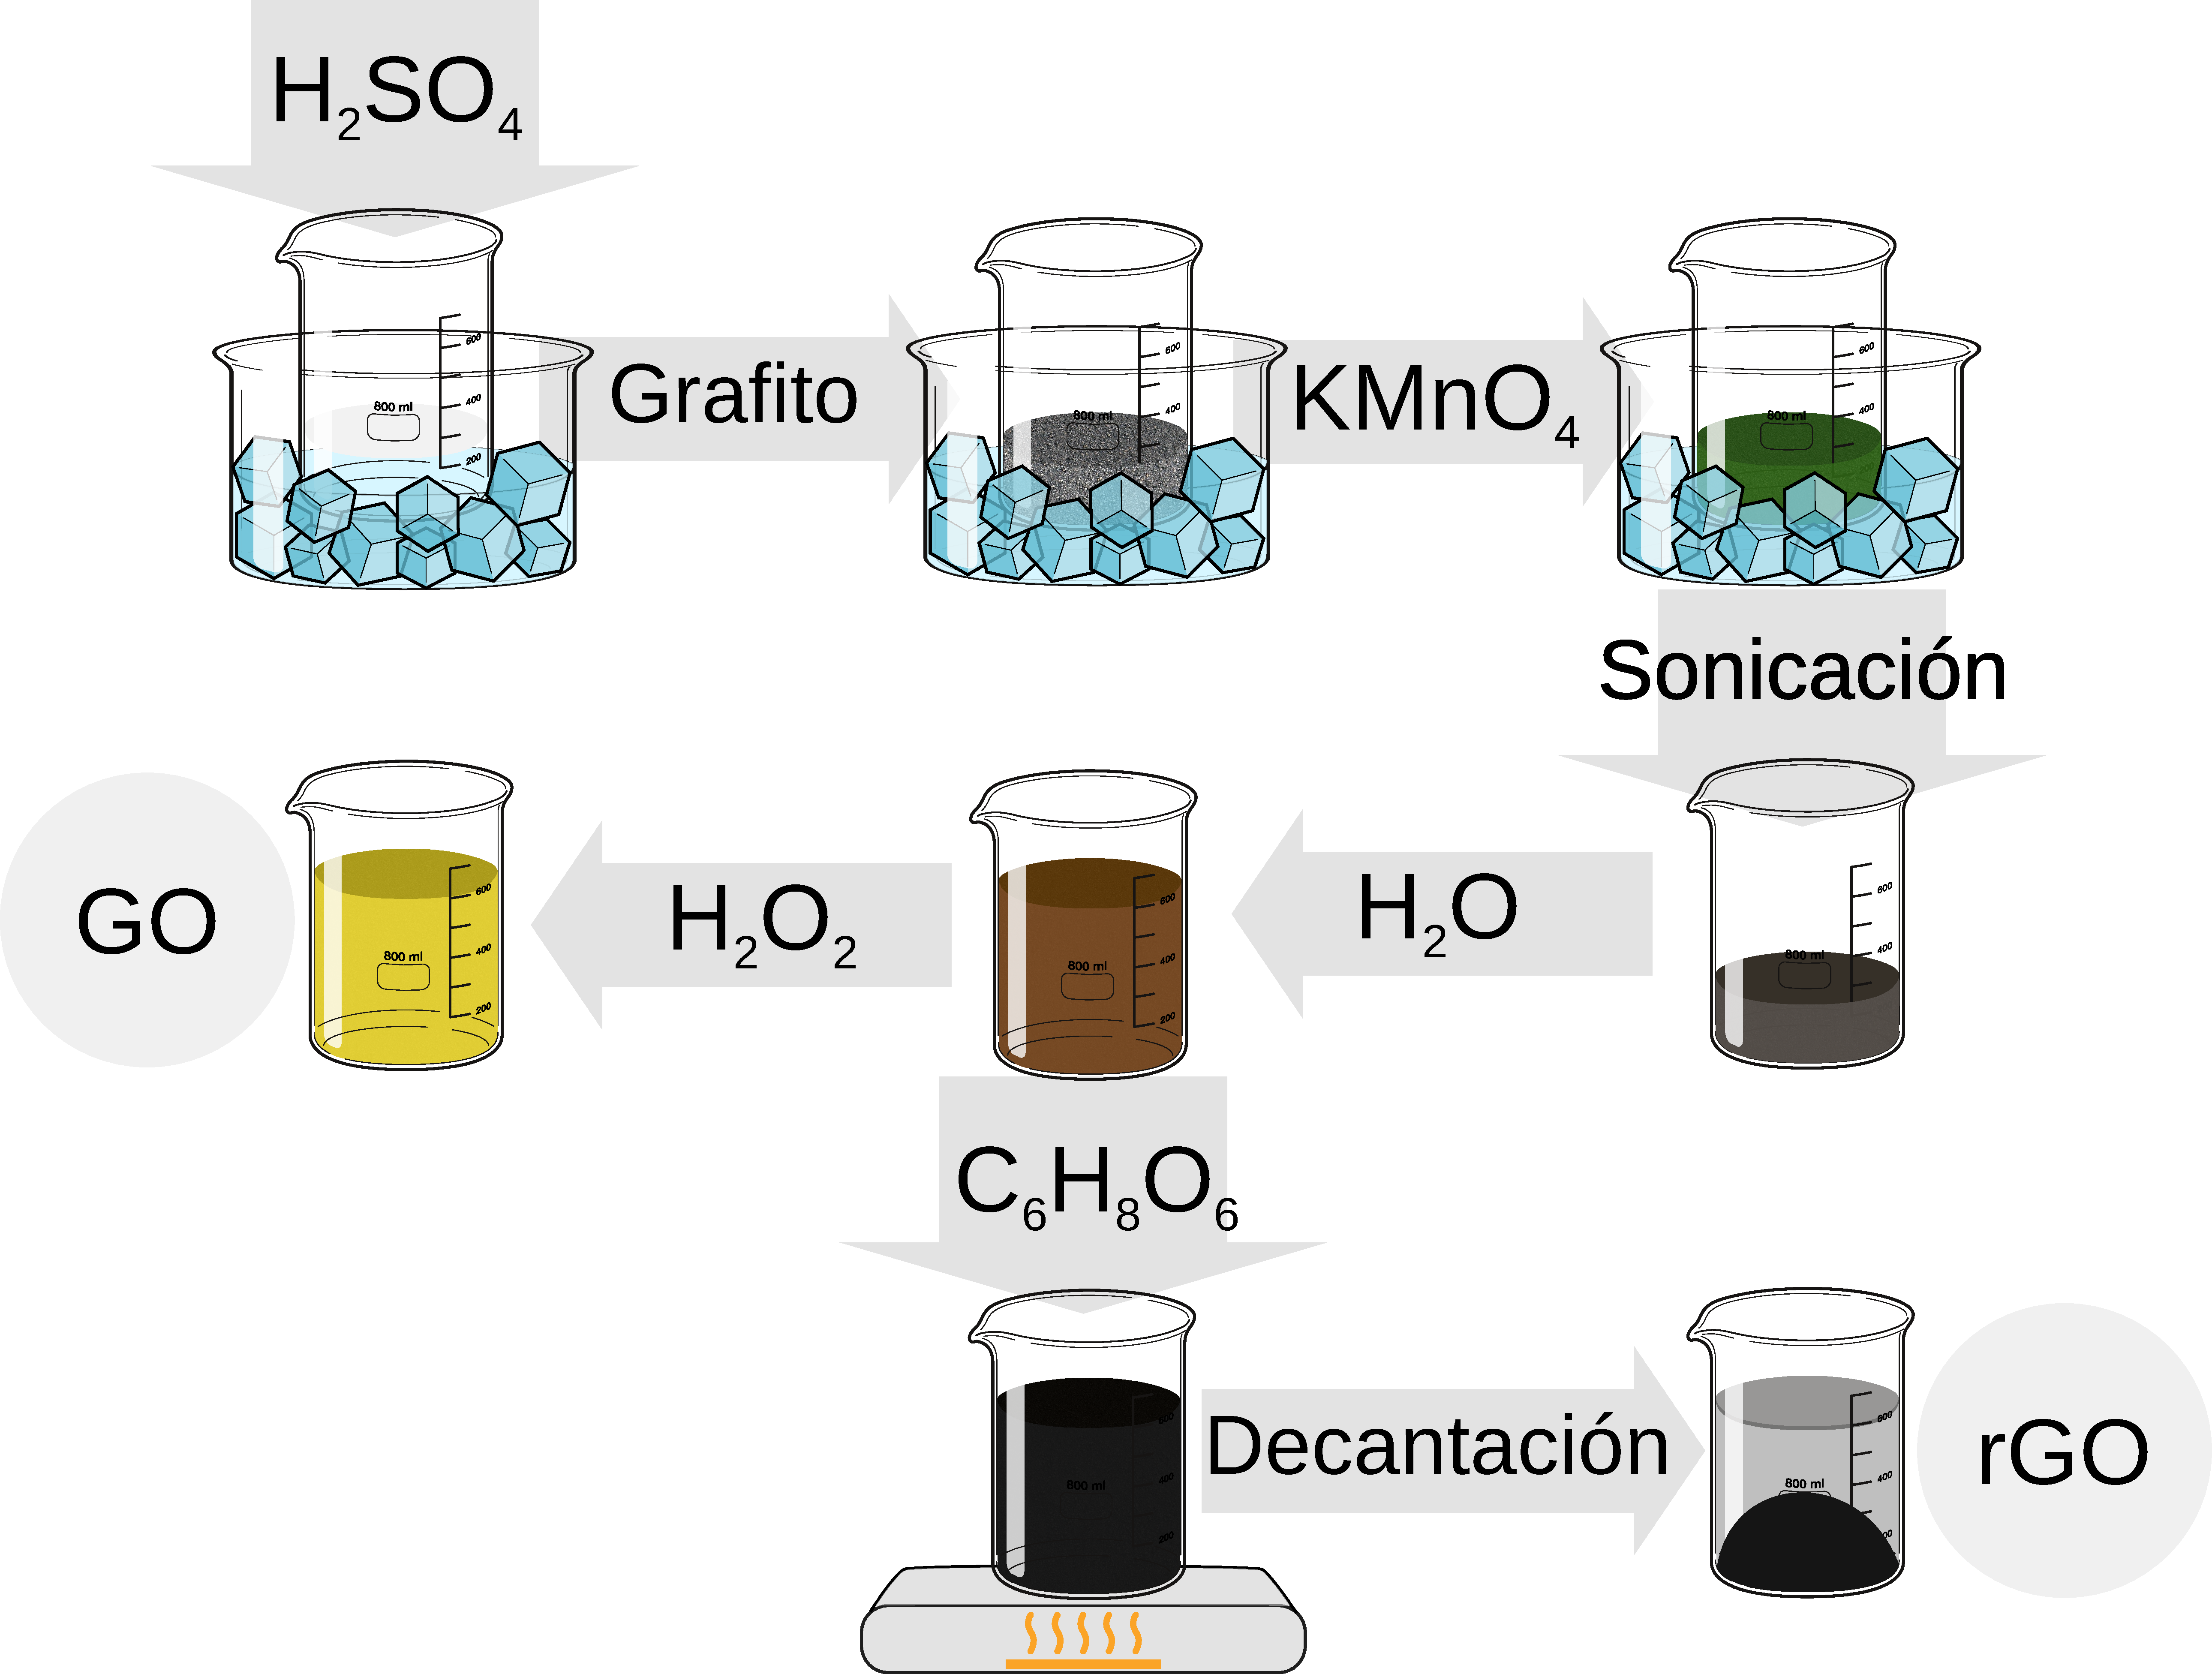
\includegraphics[width=0.7\textwidth]{experimental_method.pdf}};
					\end{scope}}
				\only<3->{\begin{scope}
					\node[] at (6, 3) {\ce{Mn2O7}};
					\node[scale=1] at (6, 2) {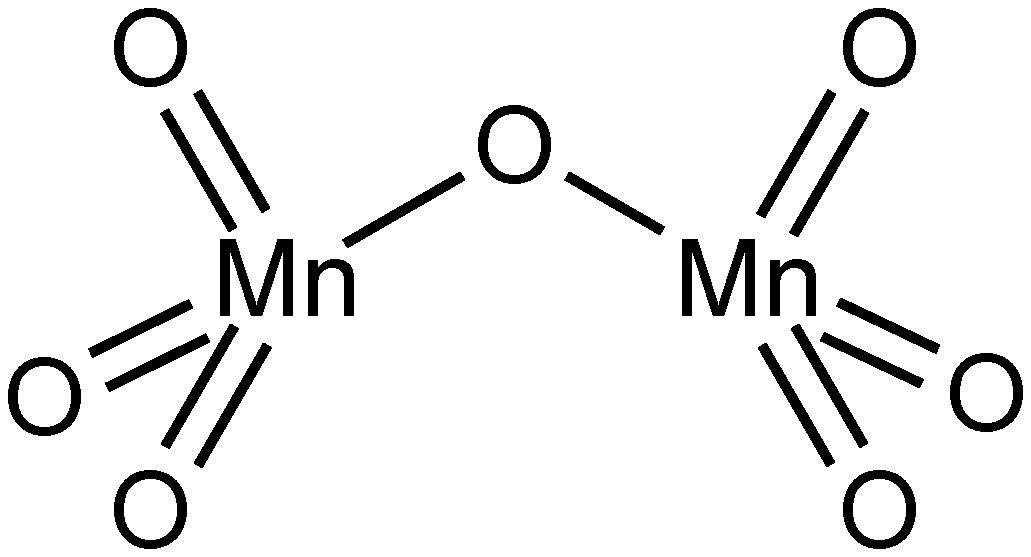
\includegraphics[width=2.5cm]{Mn2O7.pdf}};
					\clip[] (1, 1) rectangle (4, 4);
					\node at (0, 0) {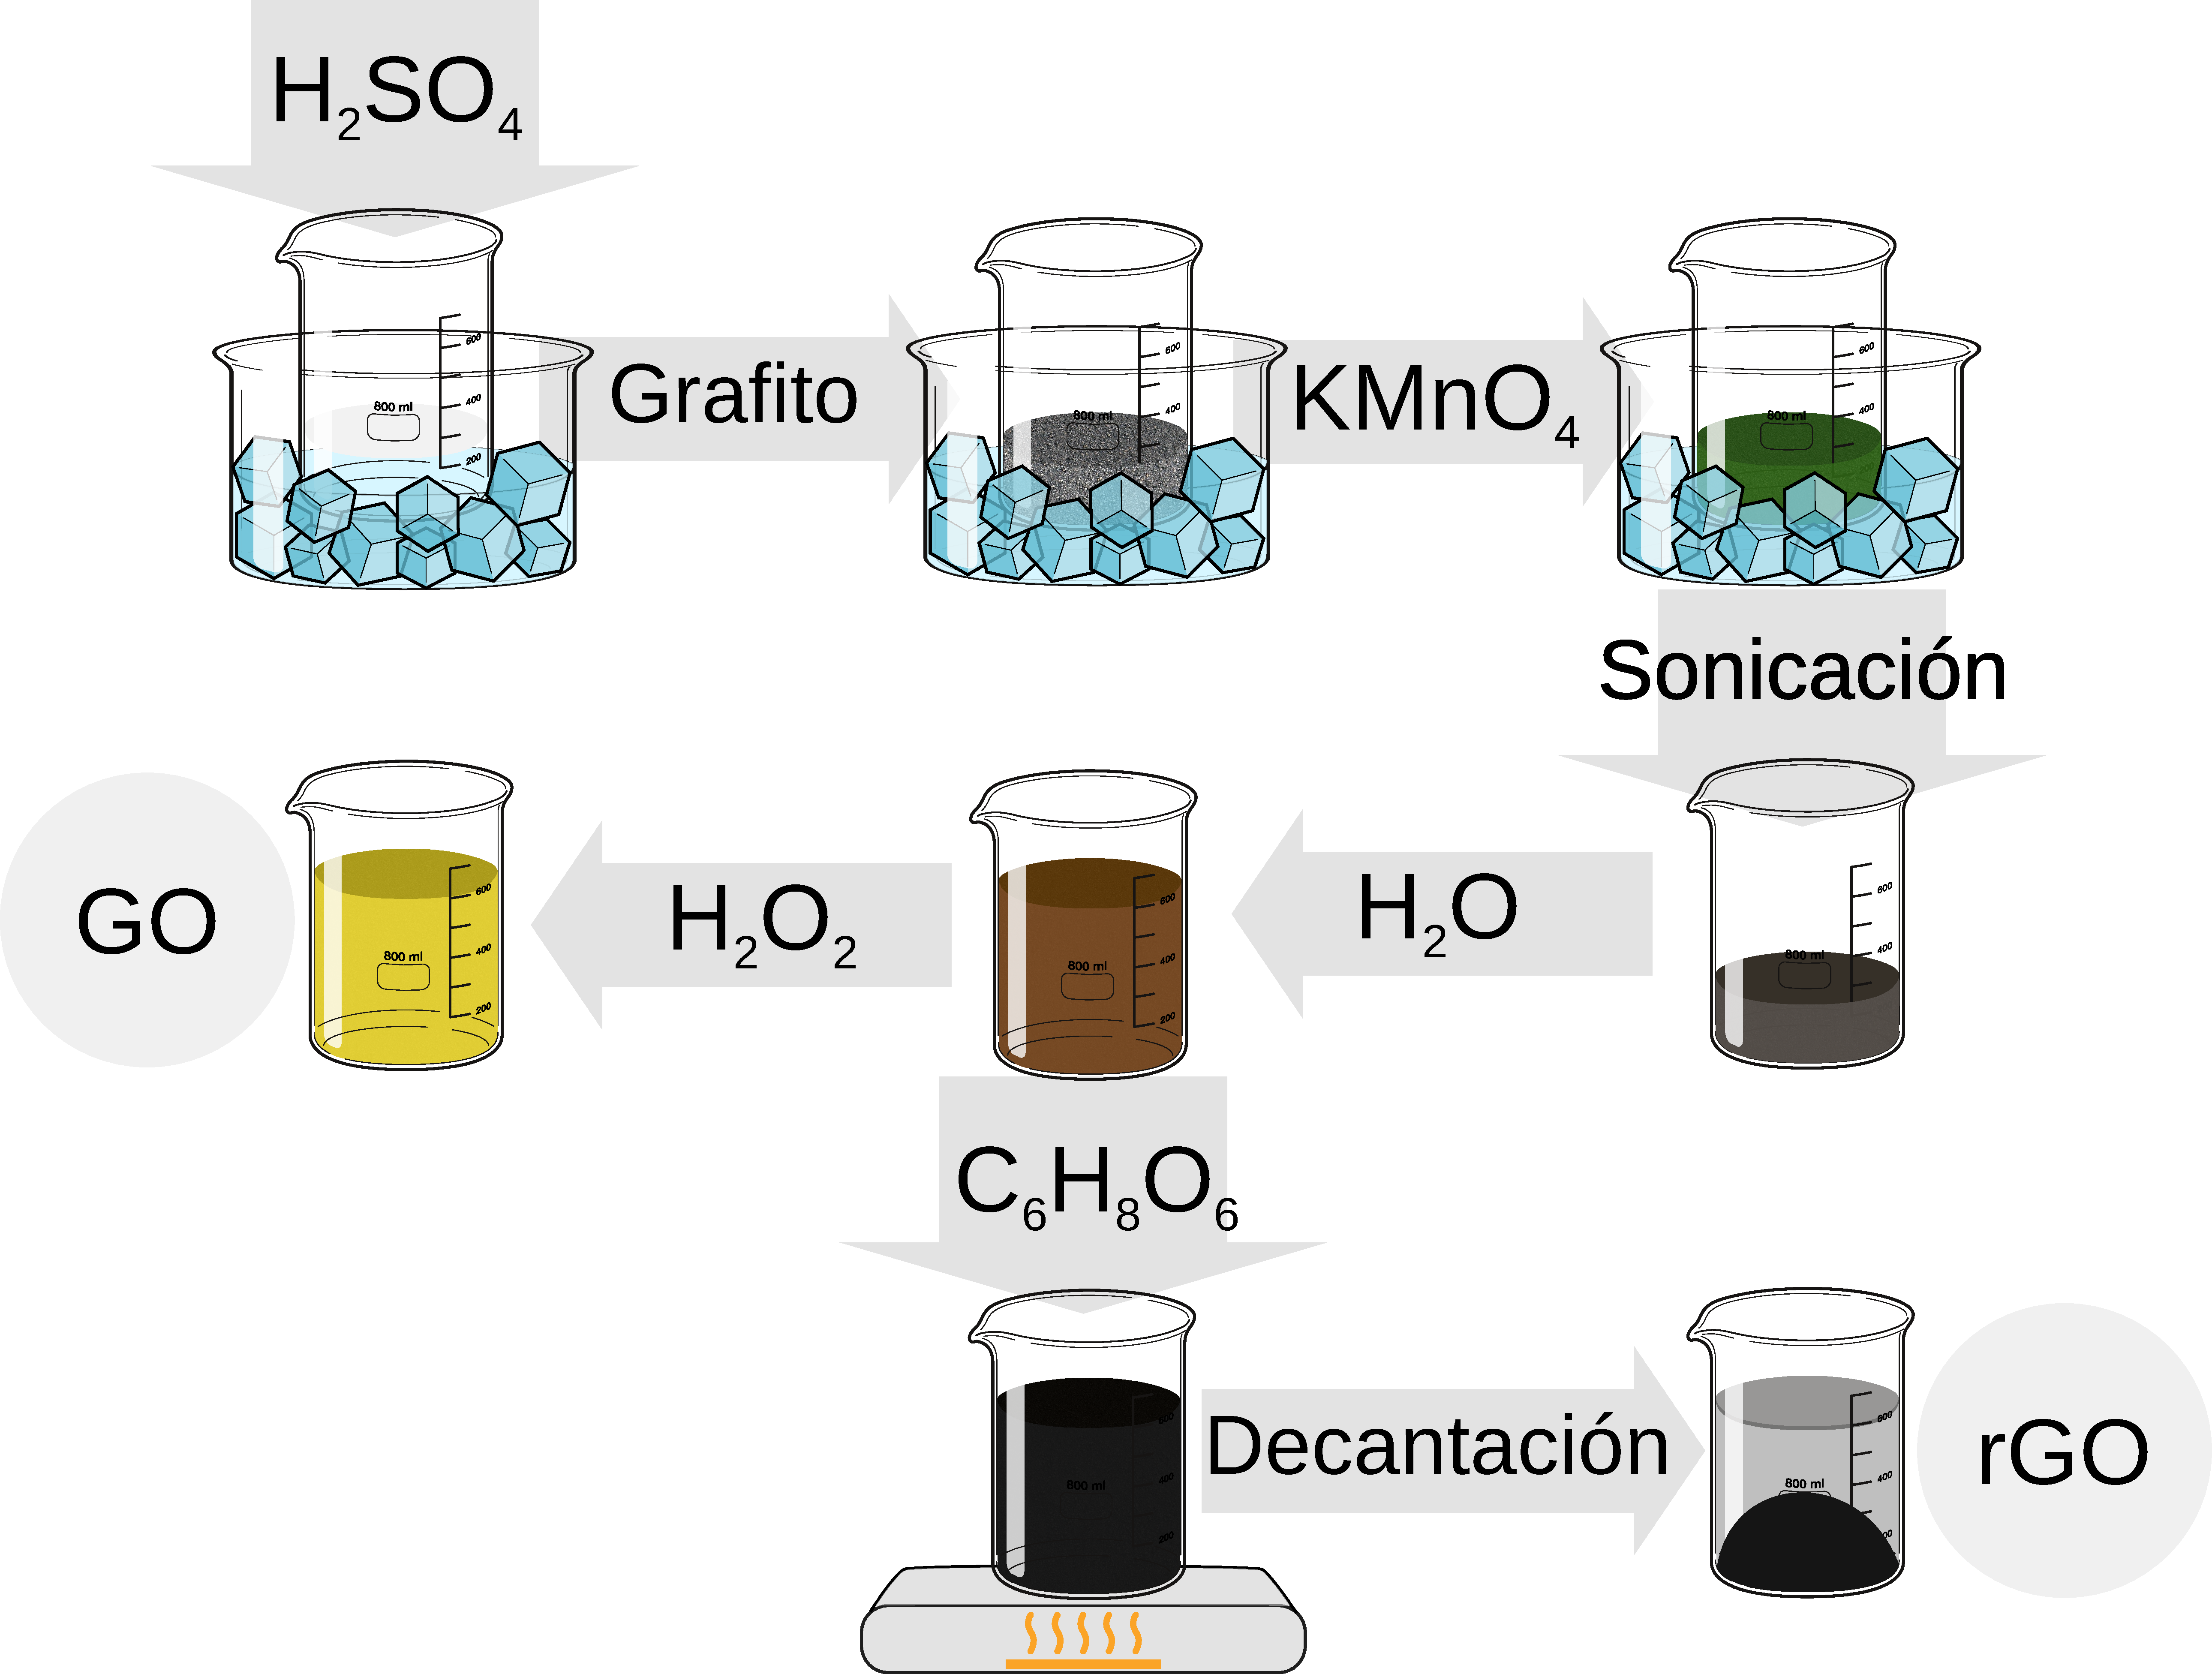
\includegraphics[width=0.7\textwidth]{experimental_method.pdf}};
					\end{scope}}
				\only<4->{\begin{scope}
					\clip[] (2, 1) rectangle (4, -1);
					\node at (0, 0) {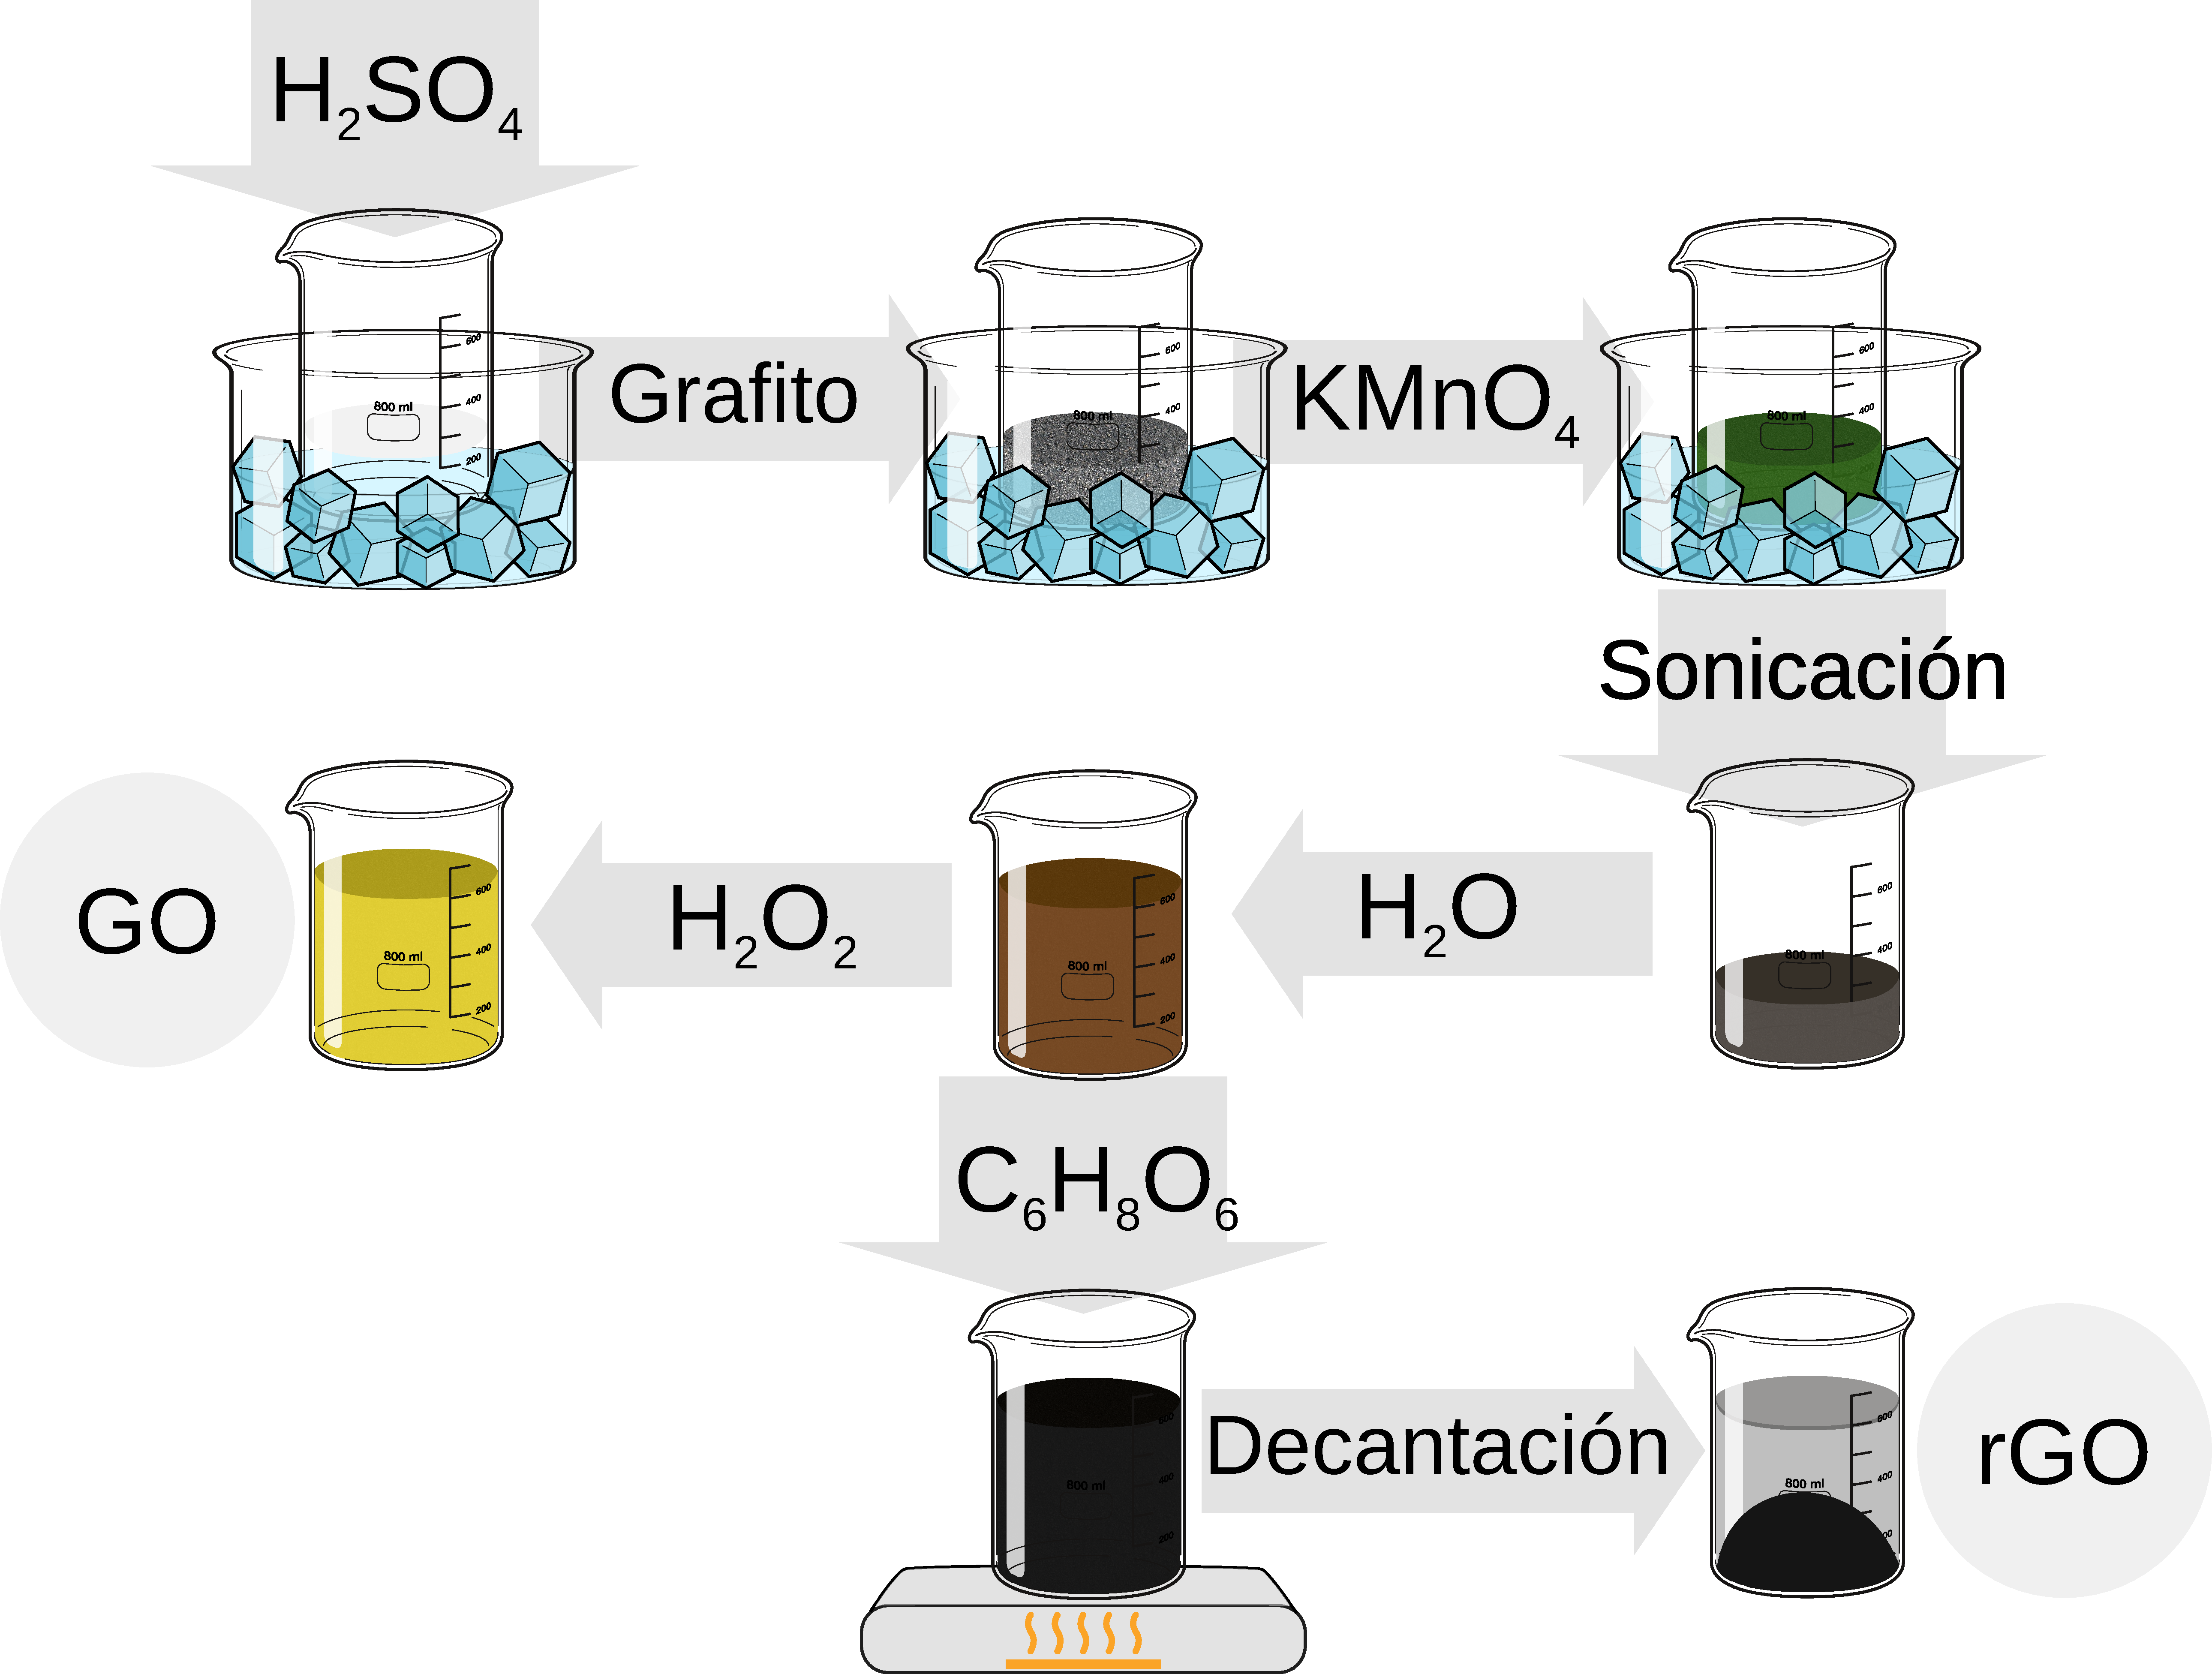
\includegraphics[width=0.7\textwidth]{experimental_method.pdf}};
					\end{scope}}
				\only<5->{\begin{scope}
					\clip[] (2, 1) rectangle (-1, -1.2);
					\node at (0, 0) {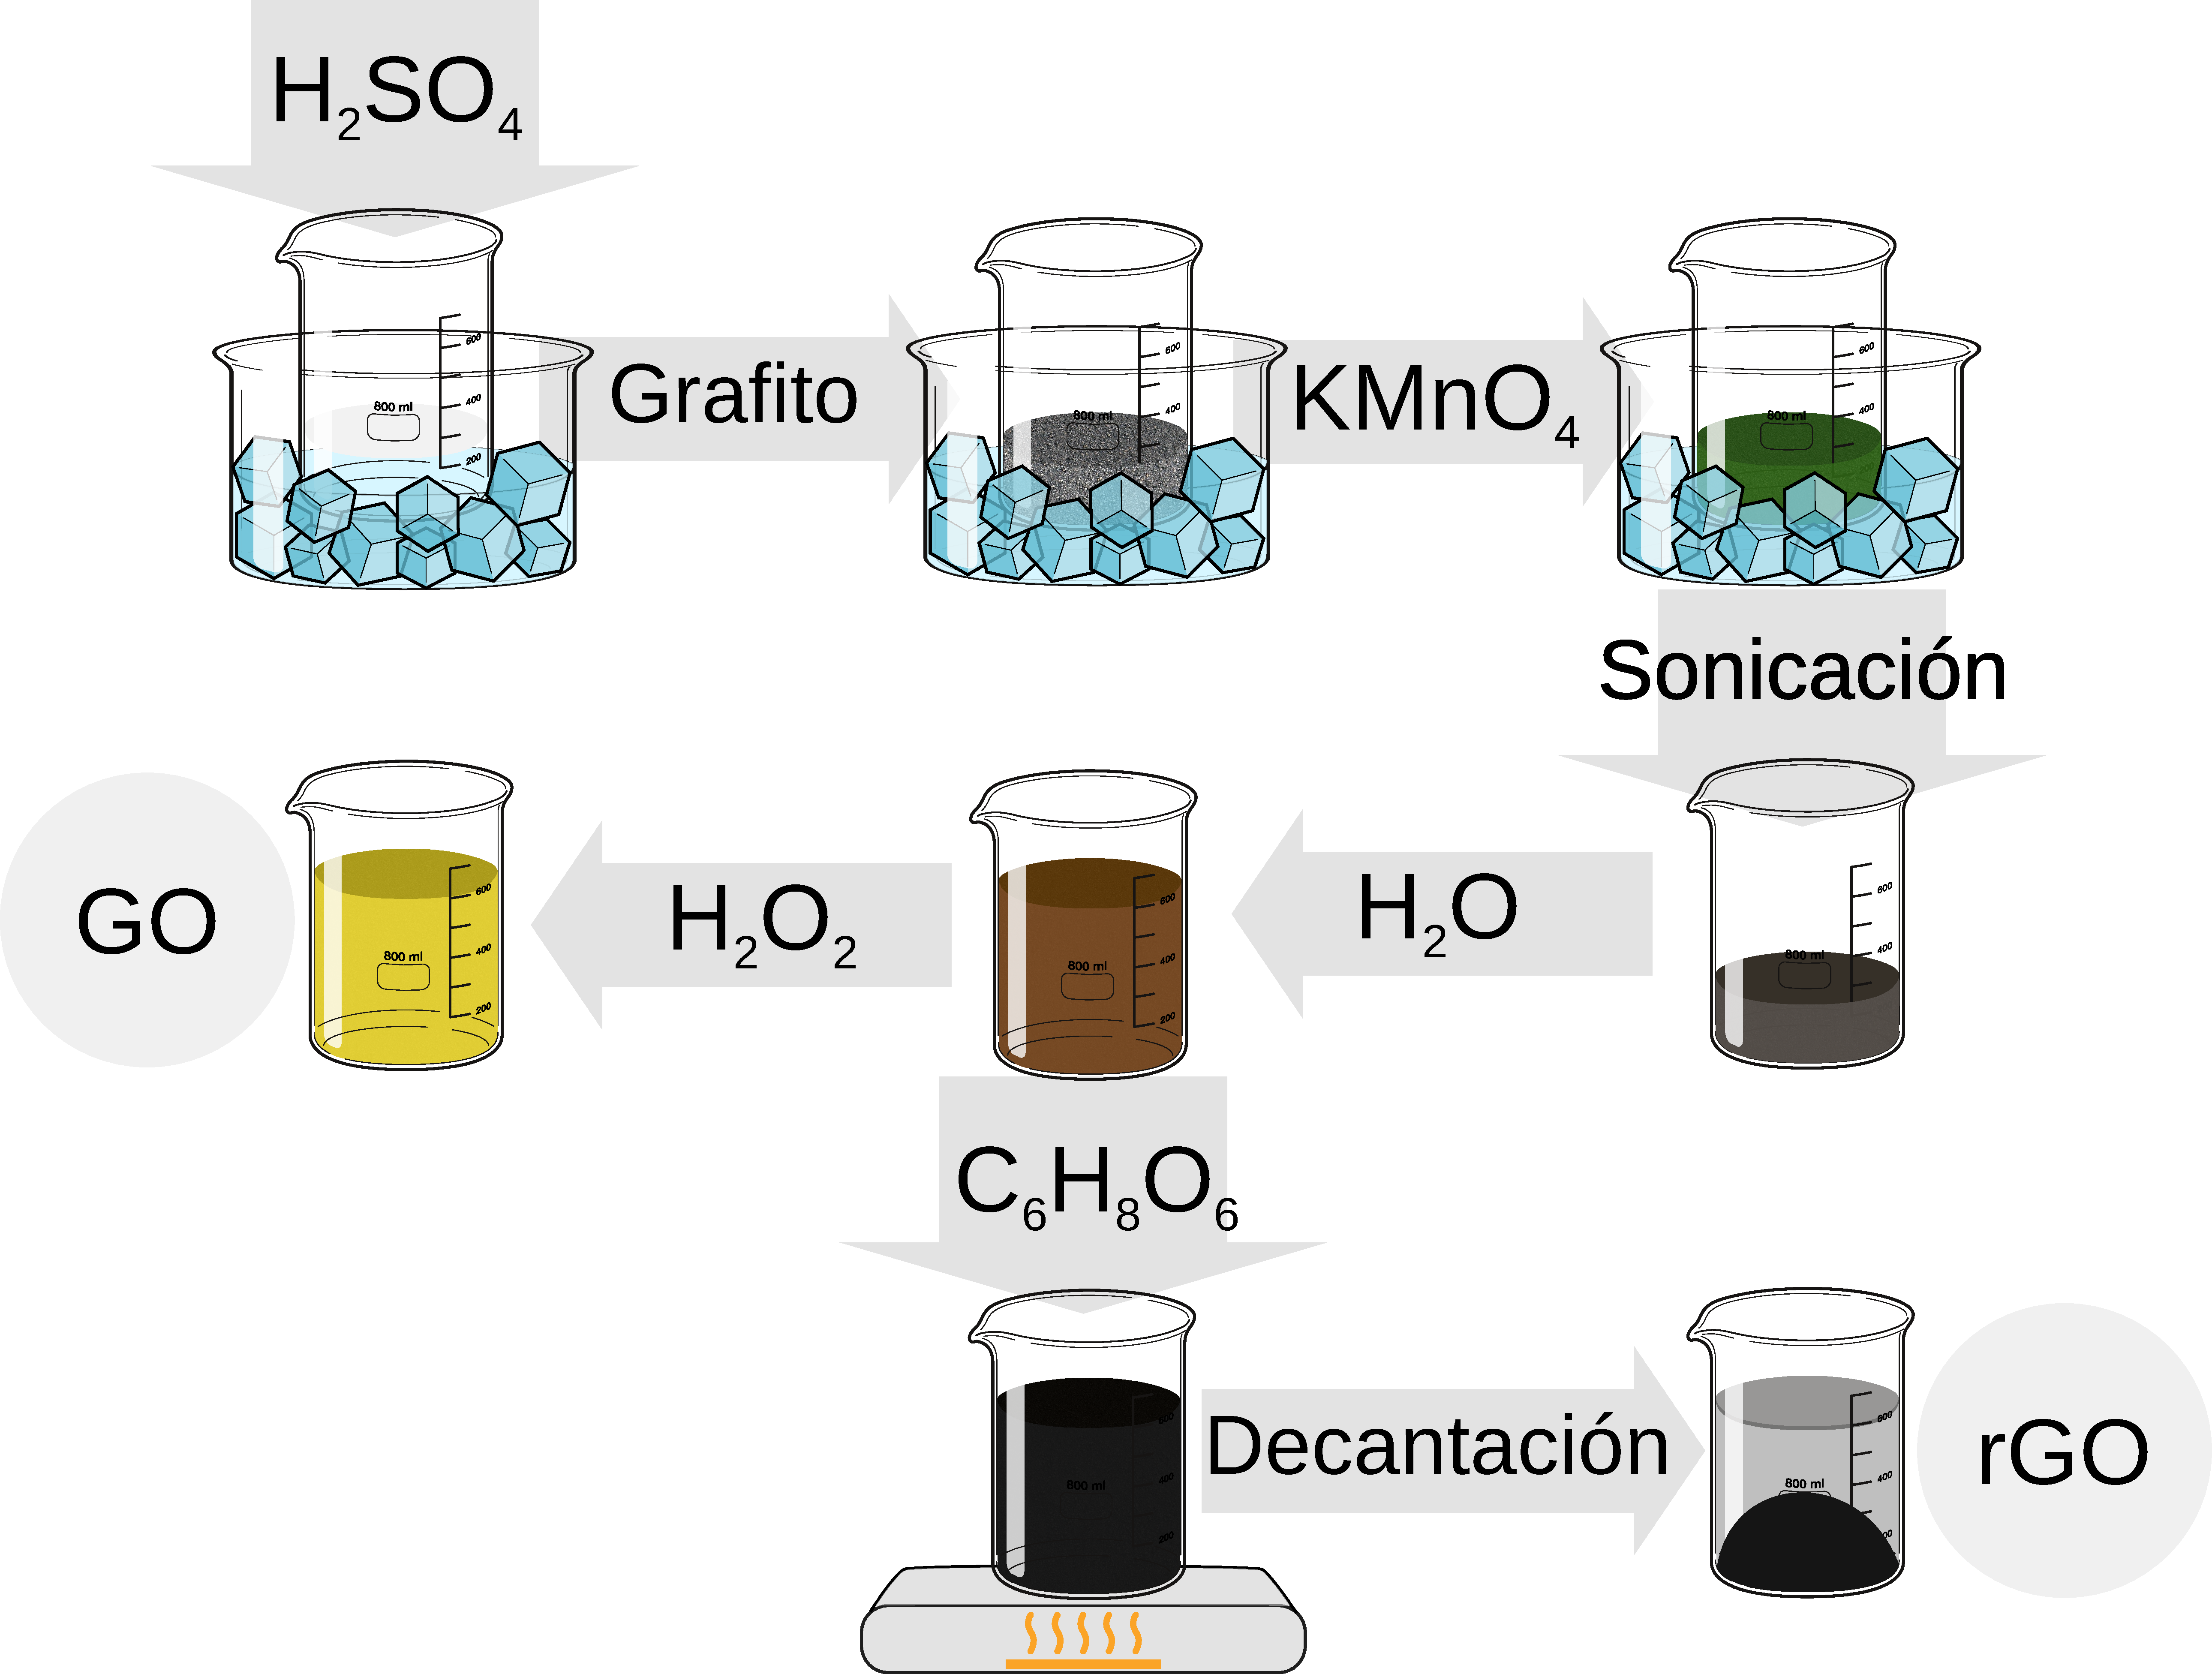
\includegraphics[width=0.7\textwidth]{experimental_method.pdf}};
				\end{scope}}
				\only<6->{\begin{scope}
					\node at (-6, -1) {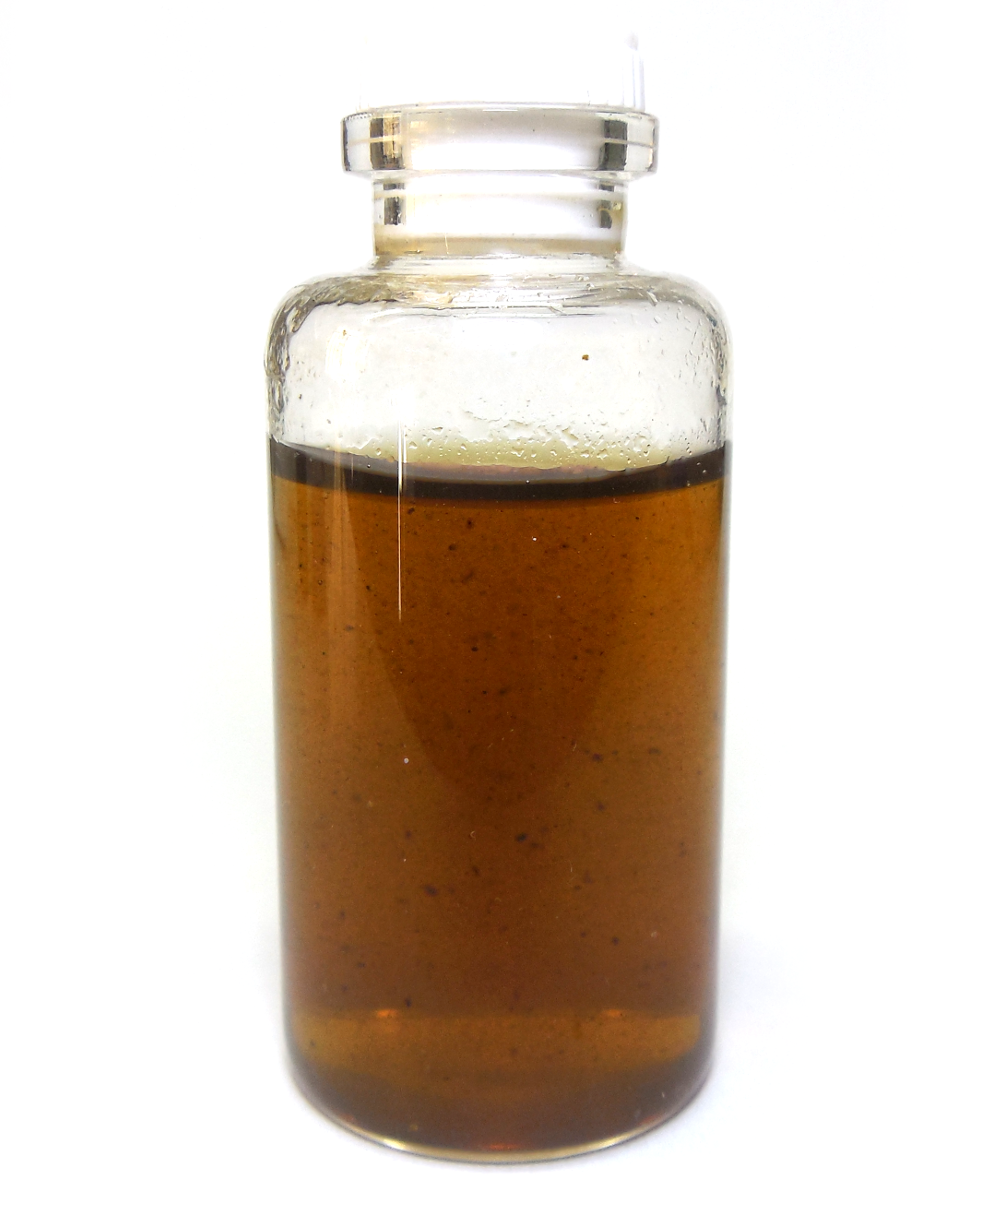
\includegraphics[width=0.3\textwidth]{GO_pic.png}};
					\clip[] (-1,1) rectangle (-5, -1.2);
					\node at (0, 0) {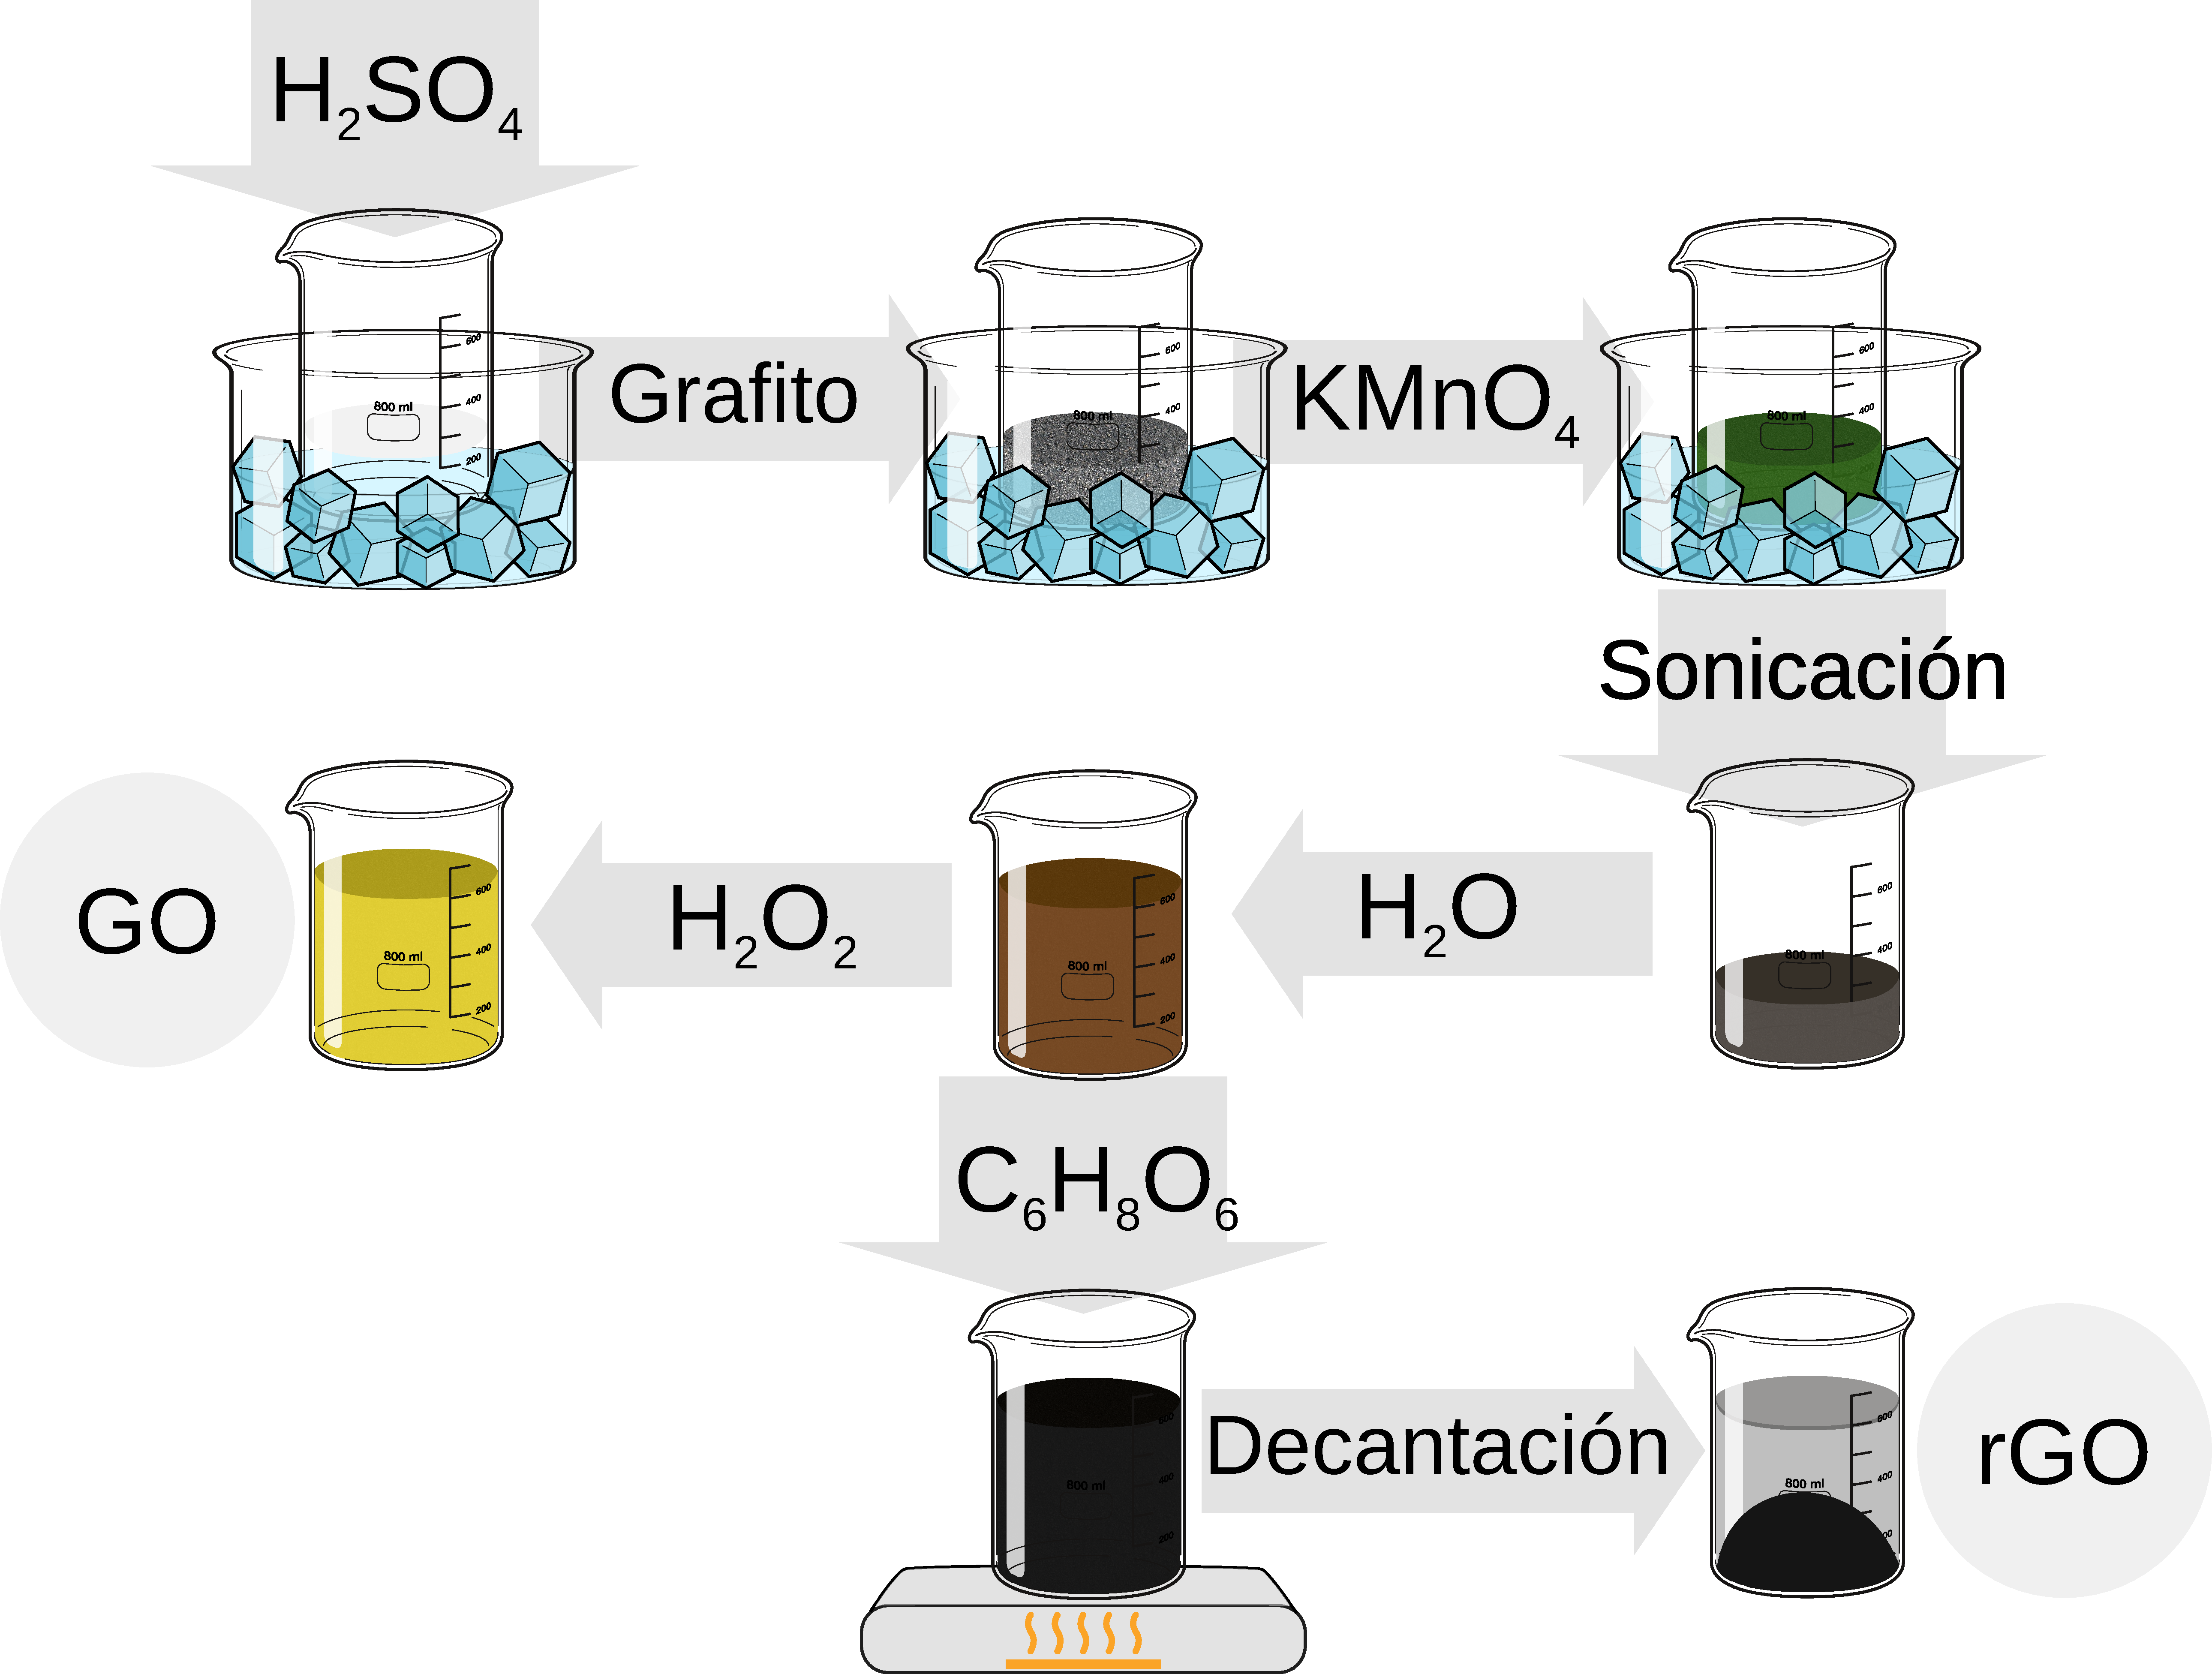
\includegraphics[width=0.7\textwidth]{experimental_method.pdf}};
					\end{scope}}
				\only<7->{\begin{scope}
					\clip[] (1, -1.2) rectangle (-2, -5);
					\node at (0, 0) {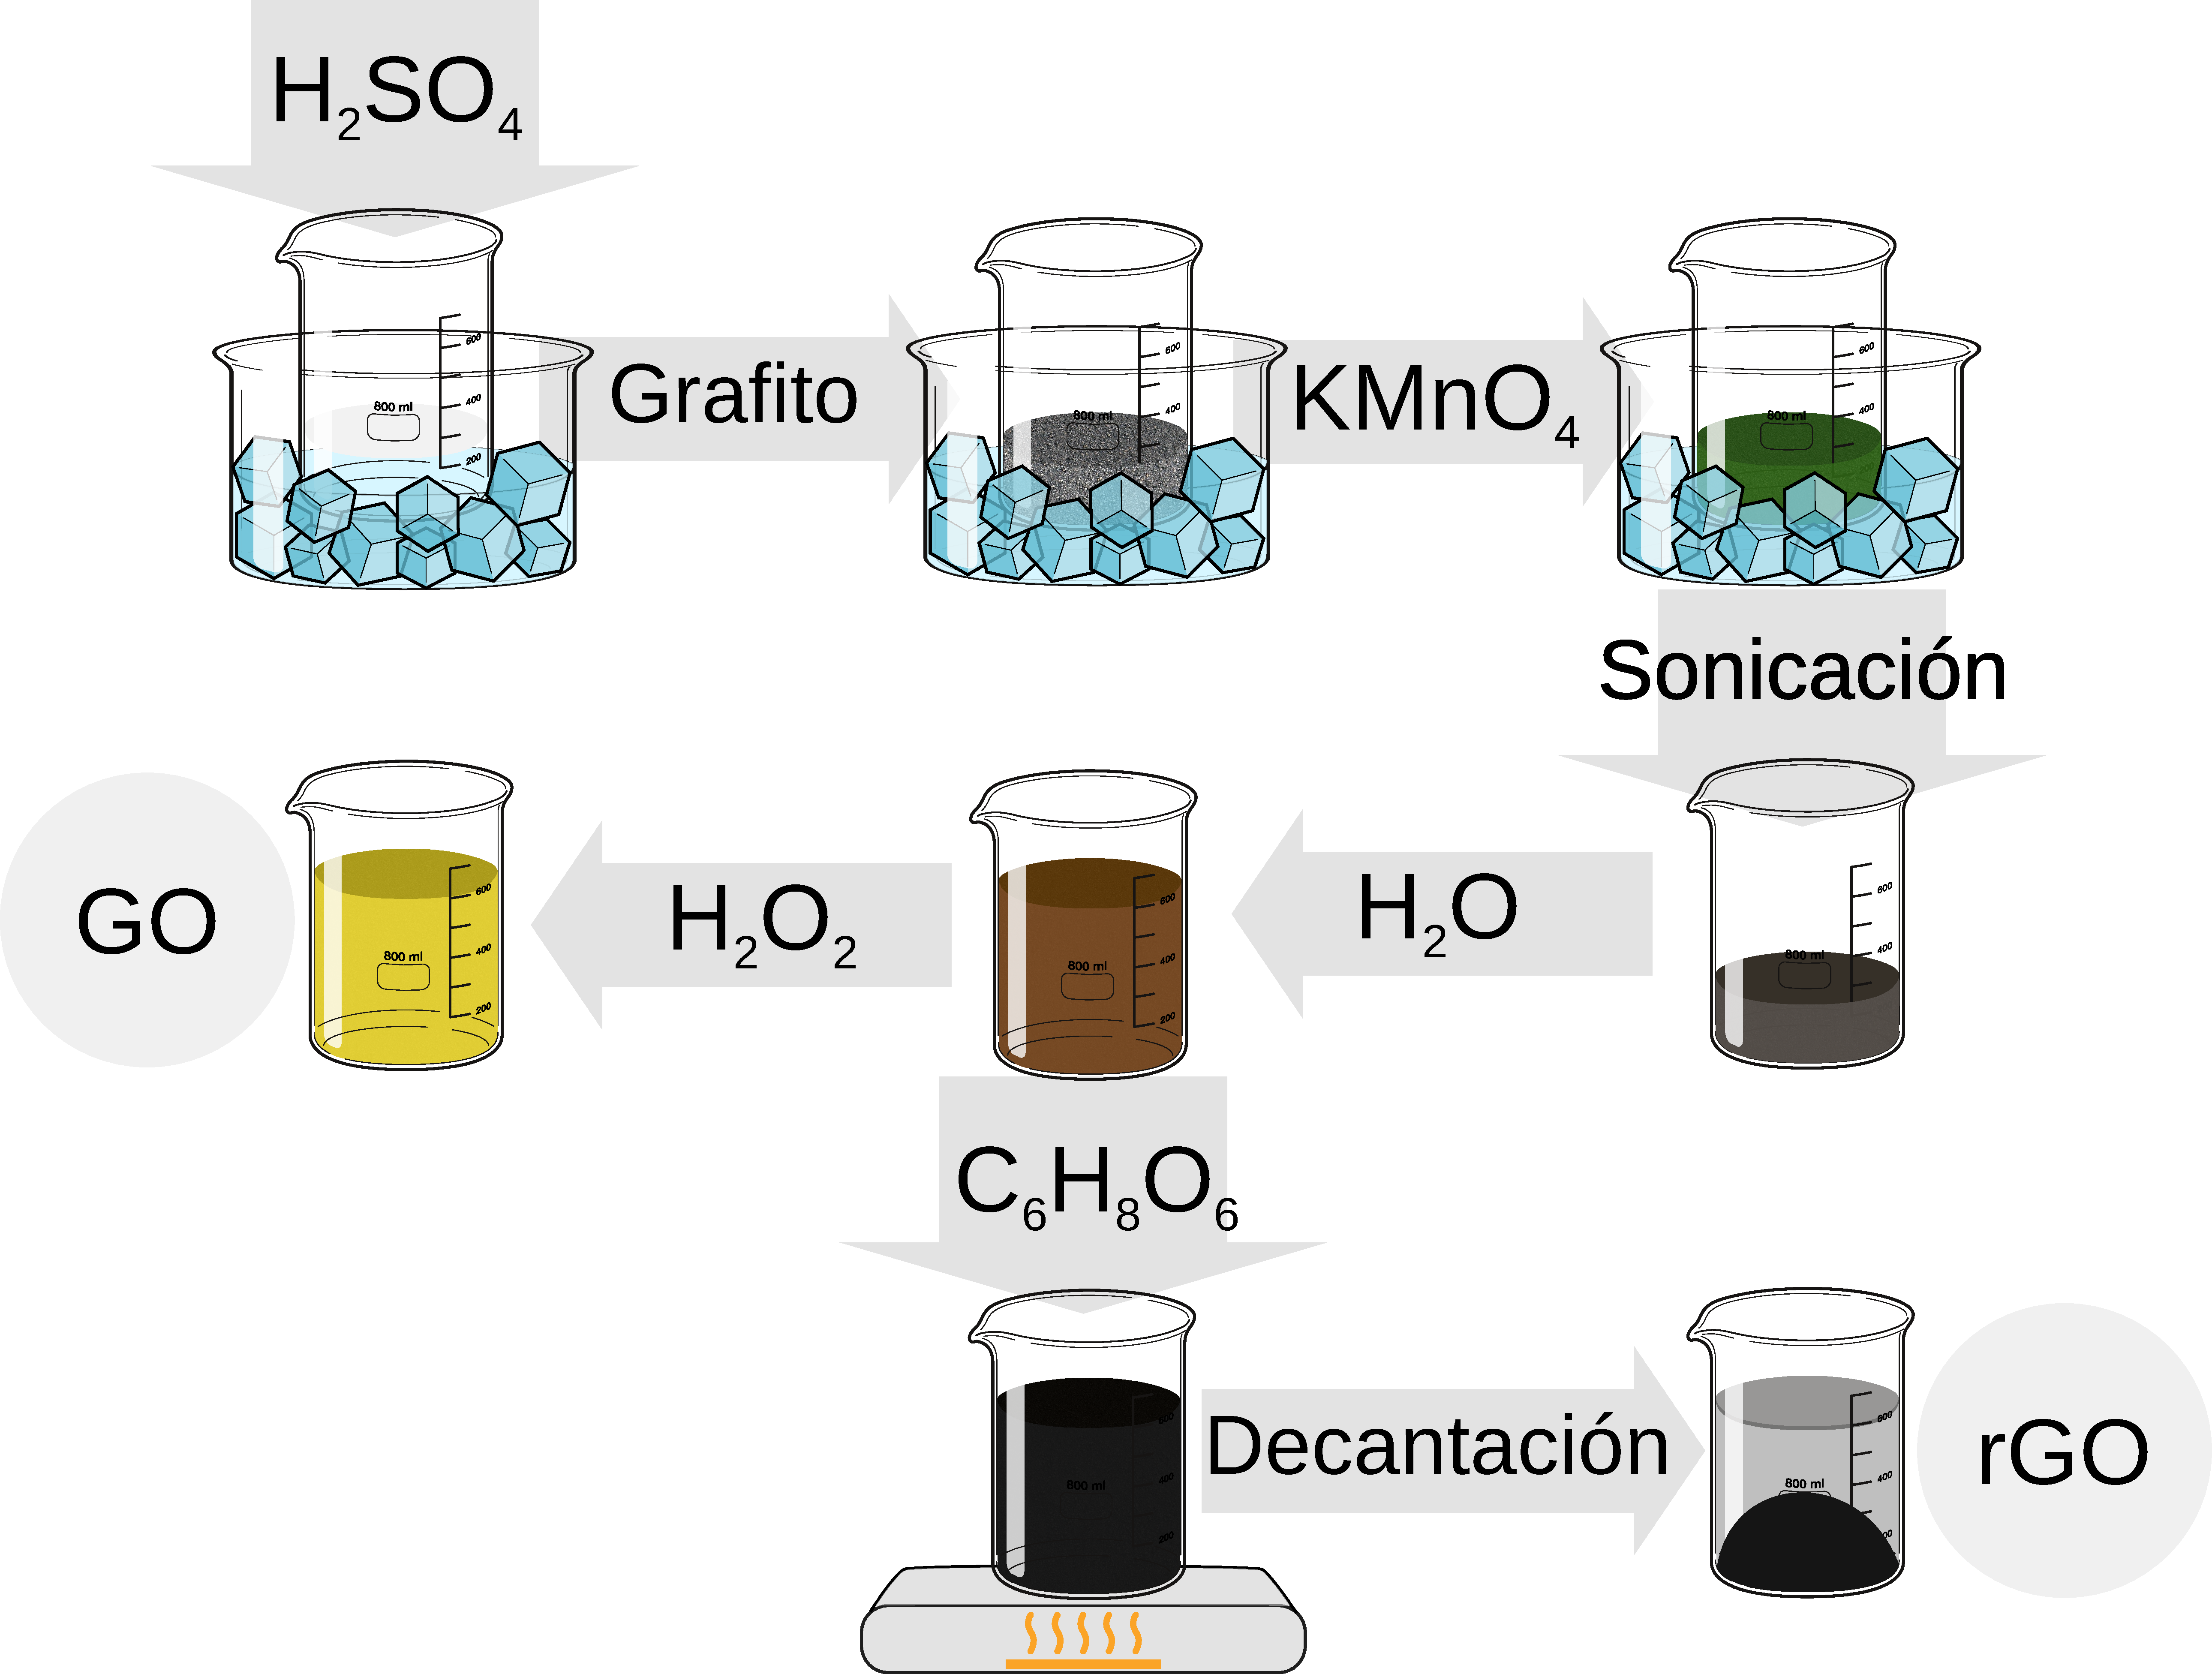
\includegraphics[width=0.7\textwidth]{experimental_method.pdf}};
					\end{scope}}
				\only<8->{\begin{scope}
					\node at (6, -2) {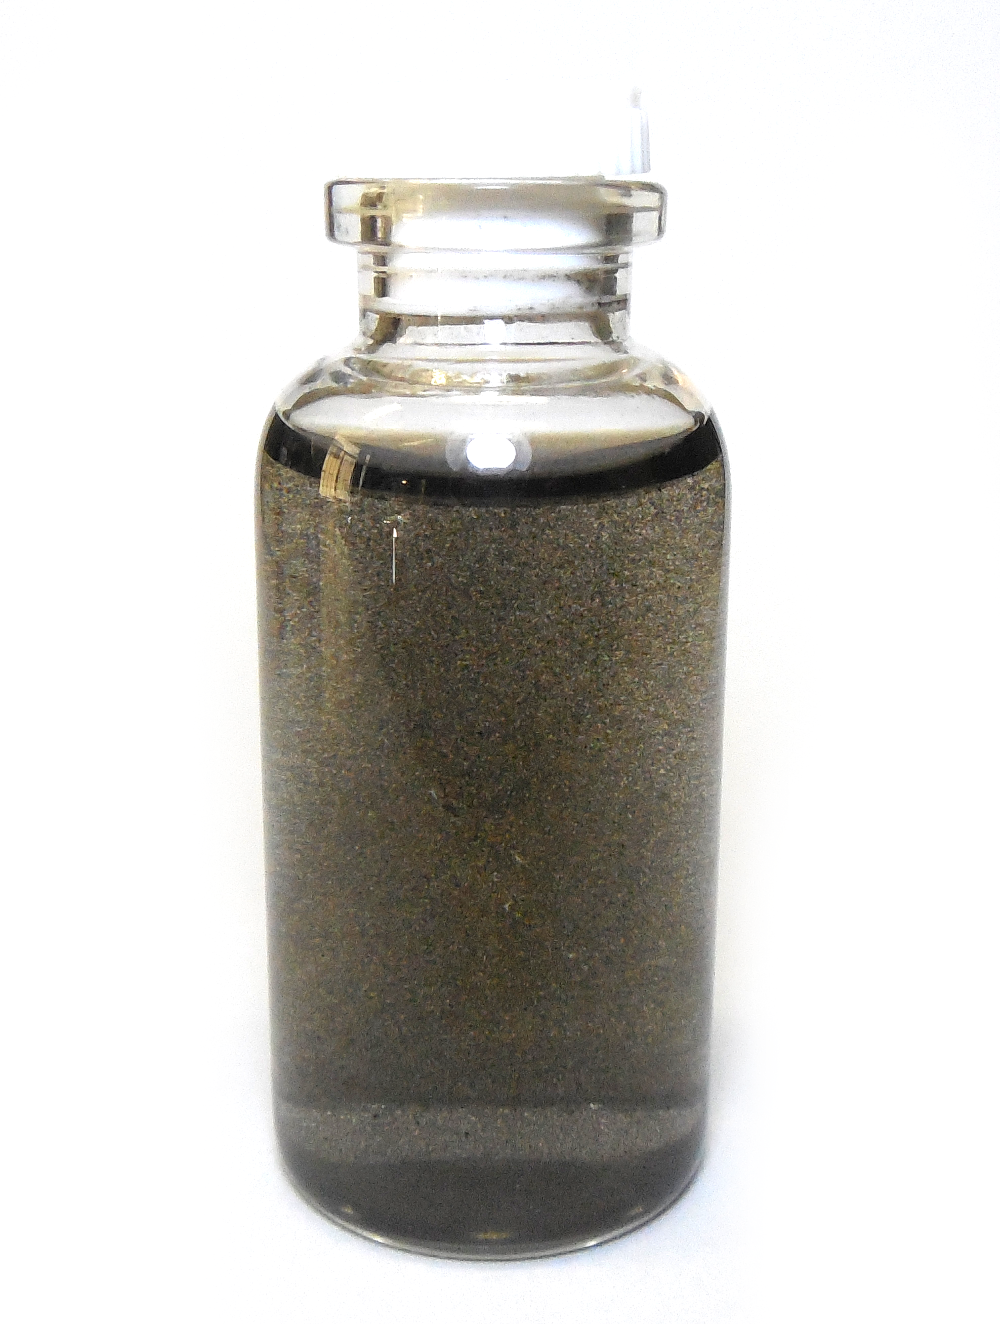
\includegraphics[width=0.3\textwidth]{RGO_pic.png}};
					\clip[] (1, -1.2) rectangle (5, -5);
					\node at (0, 0) {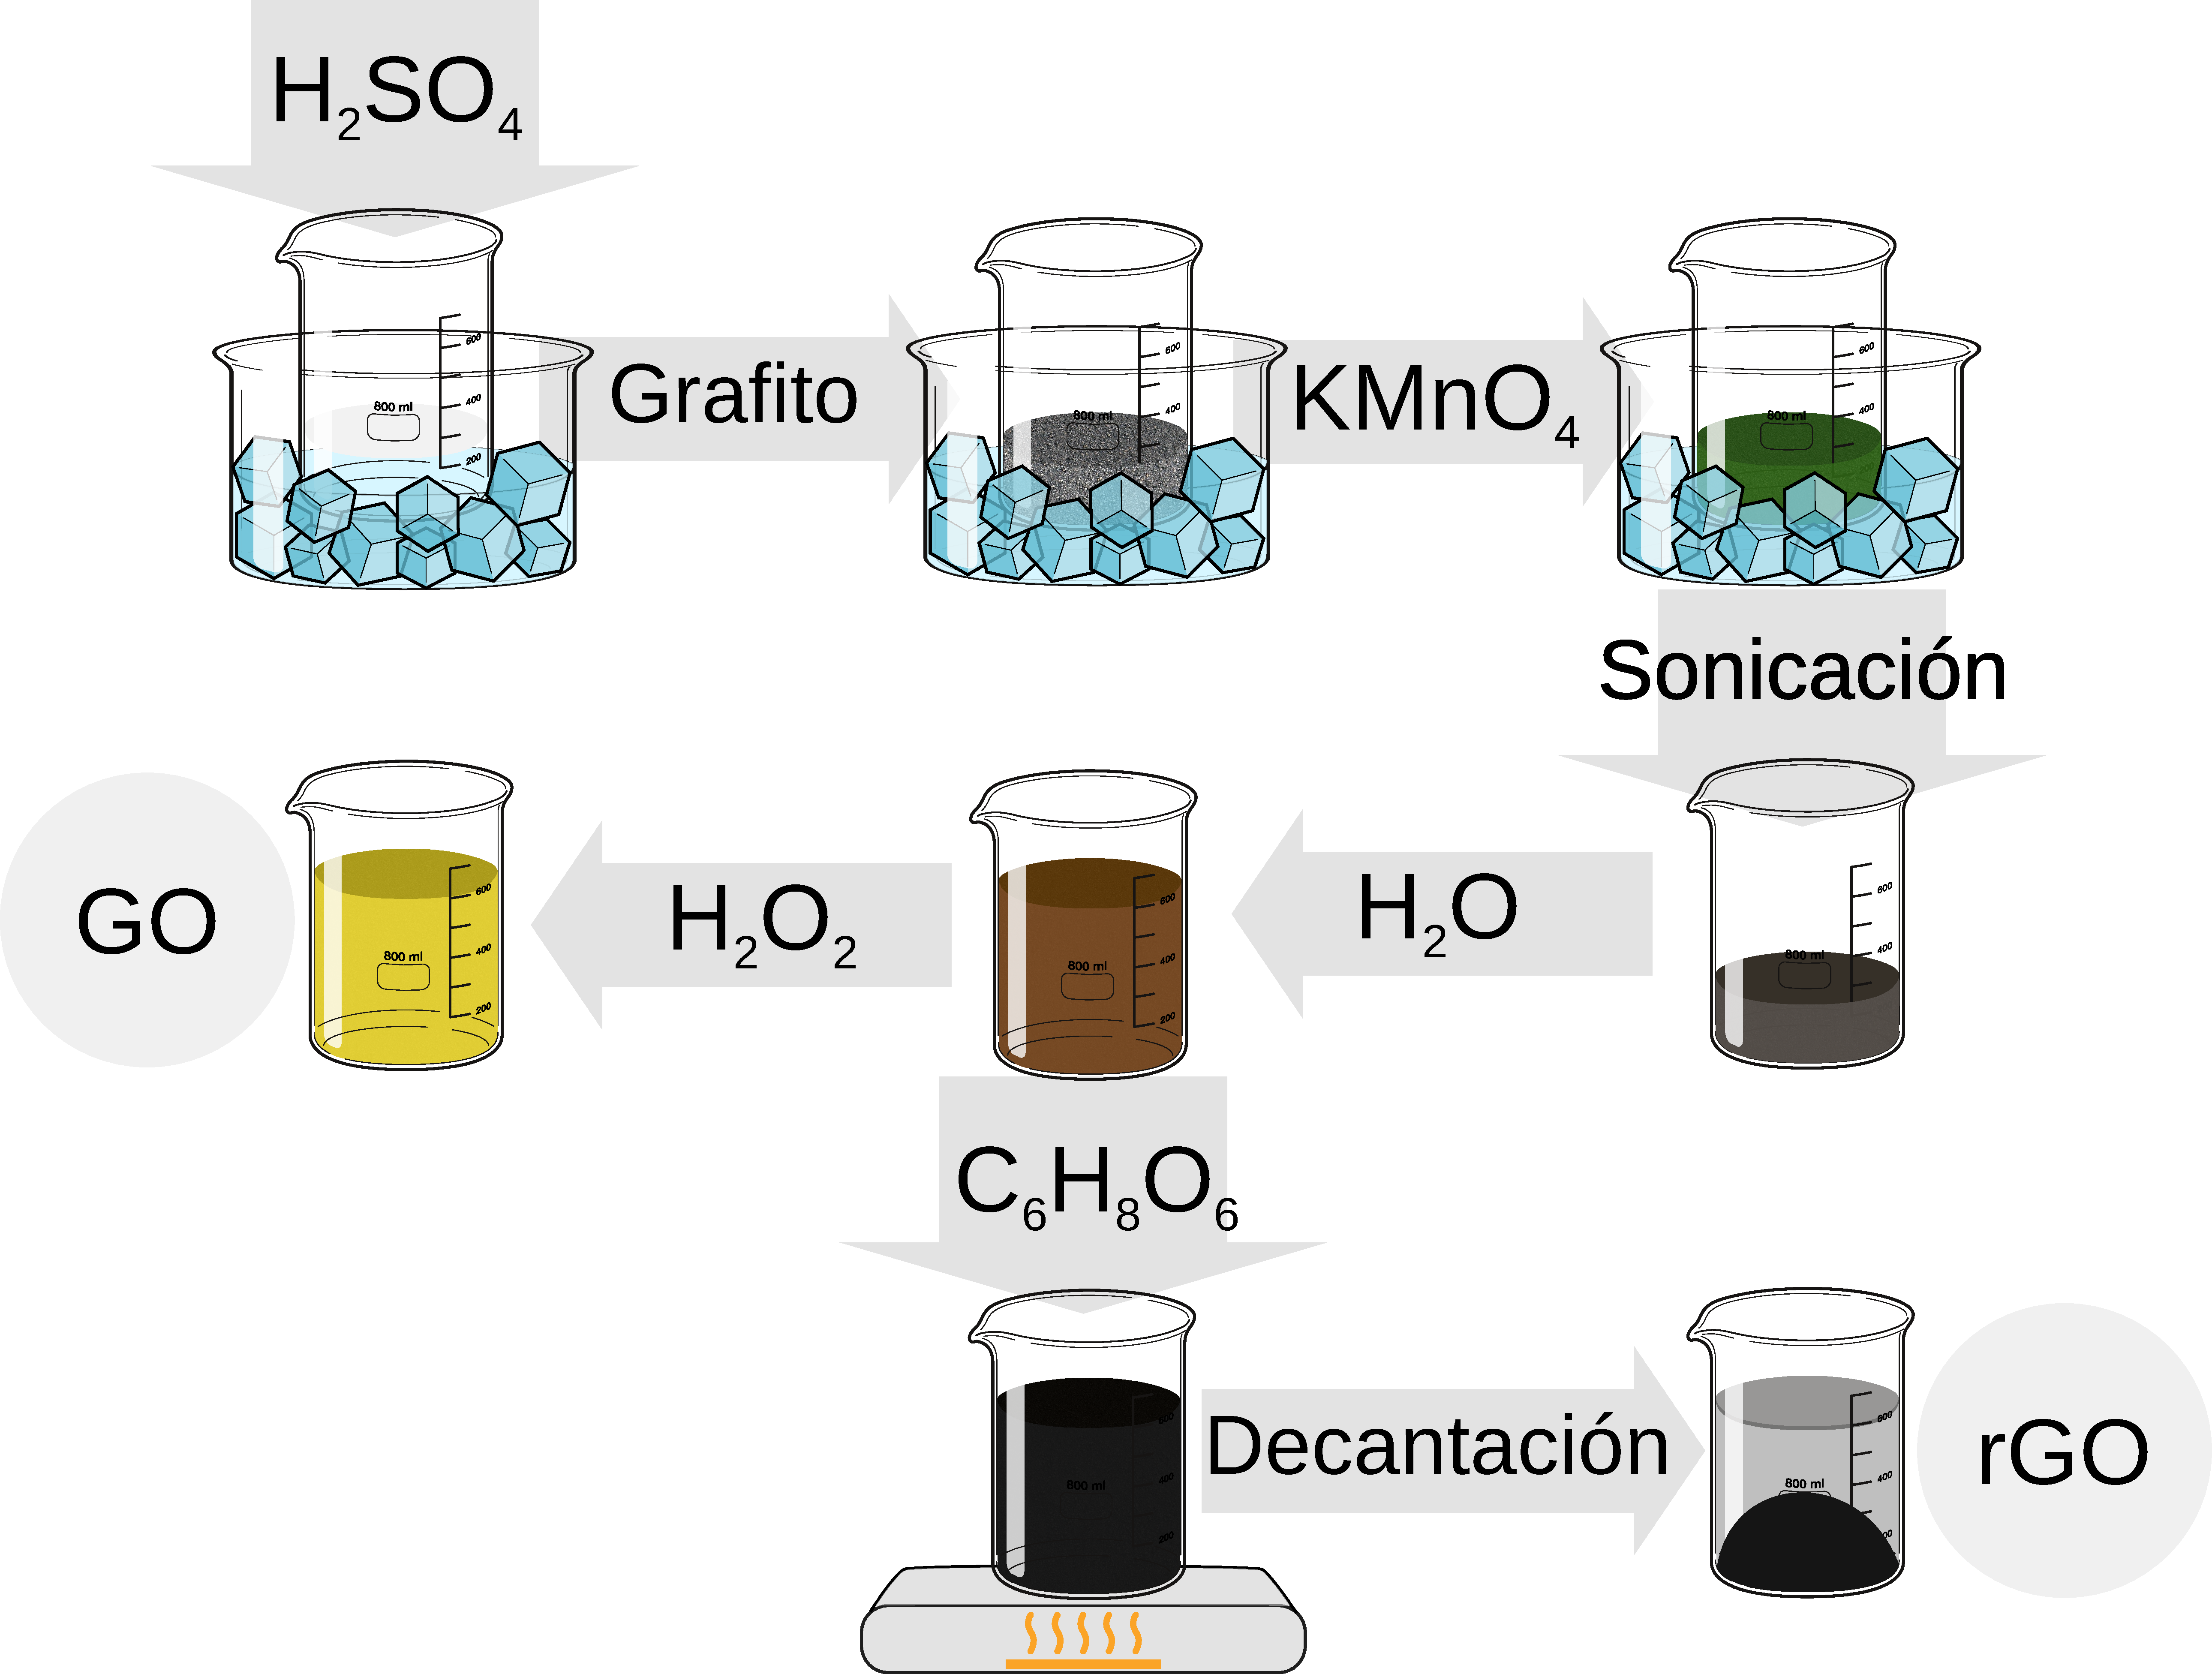
\includegraphics[width=0.7\textwidth]{experimental_method.pdf}};
					\end{scope}}
			\end{tikzpicture}
		\end{figure}
	\end{frame}	
	
	\begin{frame}{XRD}
		\begin{columns}
			\begin{column}[]{0.3\textwidth}
				\only<1->\textbf{Difracción de rayos X}
				\begin{itemize}[<+(1)->]
					\item {\textcolor{RYB1}{\textbf{Grafito:}} \\26,2\degree $\,\to\,$ 0,34 nm.}
					\item {\textcolor{RYB2}{\textbf{Óxido de grafeno:}} \\10,2\degree $\,\to\,$ 0,87 nm.}
					\item {\textcolor{RYB4}{\textbf{Óxido reducido de grafeno:}} \\22,6\degree $\,\to\,$ 0,39 nm.}
				\end{itemize}
			\end{column}
			\begin{column}[]{0.6\textwidth}
				\begin{figure}[t]
					\begin{tikzpicture}
						\begin{axis}[
						cycle list name=colorbrewer-RYB,
						no markers,
						width=\textwidth,
						height=0.9*\axisdefaultheight,
						yticklabels={,,},
						ylabel={Intensidad},
						y unit=u.a.,
						xlabel={2$\mathrm{\theta}$},
						x unit=grados,
						every axis legend/.append style={
							font={\normalsize}, 
							at={(0.5,1.05)},
							anchor=north west,
						},
						legend entries={Grafito, Óxido de grafeno, Óxido de grafeno reducido},
						]
						\addplot table [x expr = \thisrow{2t}, y expr=\thisrow{C}] {./Data/XRD/xrd.txt};
						\addplot table [x expr = \thisrow{2t}, y expr=\thisrow{GO}+1] {./Data/XRD/xrd.txt};
						\pgfplotsset{cycle list shift=1}
						\addplot table [x expr = \thisrow{2t}, y expr=\thisrow{RGO}+2] {./Data/XRD/xrd.txt};
						\end{axis}
					\end{tikzpicture}
					\caption[]{Espectro de difracción de rayos x.}
				\end{figure}
			\end{column}
		\end{columns}
	\end{frame}

	\begin{frame}{Raman}
		\begin{columns}
			\begin{column}[]{0.4\textwidth}
				\textbf{Espectro Raman}
				\begin{itemize}
					\item La relación de intensidades entre bandas $I_D/I_G$ se incrementa con los defectos en la red.
					\item \textcolor{RYB2}{Óxido de grafeno:\\$I_D/I_G$ = 0,9.}
					\item \textcolor{RYB4}{Óxido reducido de grafeno:\\ $I_D/I_G$ = 1,3.}
					
				\end{itemize}
			\end{column}
			\begin{column}[]{0.6\textwidth}
				\begin{figure}[t]
					\centering
					\begin{tikzpicture}[]
					\begin{axis}[
					cycle list name=colorbrewer-RYB,
					no markers,
%					grid=both,
					%		yticklabels={,,},
					width = \textwidth,
					height=0.8*\axisdefaultheight,
					yticklabels={,,},
					ylabel={Intensidad},
					y unit=u.a.,
					xlabel={Corrimiento Raman},
					x unit=cm^{-1},
					every axis legend/.append style={
						font={\normalsize}, 
						at={(0.5,1.05)},
						anchor=north west,
					},
					legend entries={Óxido de grafeno, Óxido de grafeno reducido}]
						\pgfplotsset{cycle list shift=1}
						\addplot+[restrict x to domain=1000:3500] table [x expr = \thisrow{raman_shift}, y expr=\thisrow{CRGO090615_1}] {./Data/RAMAN/raman.txt};
						%		\addplot+[restrict x to domain=1000:3500] table [x expr = \thisrow{raman_shift}, y expr=\thisrow{GO090615_1} + 10] {./Data/RAMAN/raman.txt};
						\pgfplotsset{cycle list shift=2}
						\addplot+[restrict x to domain=1000:3500] table [x expr = \thisrow{raman_shift}, y expr=\thisrow{GO090615_2} + 20] {./Data/RAMAN/raman.txt};
						%	\addplot table [x expr = \thisrow{2t}, y expr=\thisrow{RGOLYO}+3] {./Data/XRD/xrd.txt};
						\node[black] at (25,1000){\small{D}};
						\node[black] at (60, 900){\small{G}};
%						\node[black] at (160, 300){\small{2D}};
					\end{axis}
					\end{tikzpicture}
					\caption[Espectro Raman de GO y rGO]{Espectro Raman de muestras de óxido de grafeno y óxido reducido de grafeno.}
				\end{figure}
			\end{column}
		\end{columns}
	\end{frame}

	\begin{frame}{Microscopía SEM}
		\begin{figure}[h]
			\centering
			\begin{subfigure}{0.45\textwidth}
				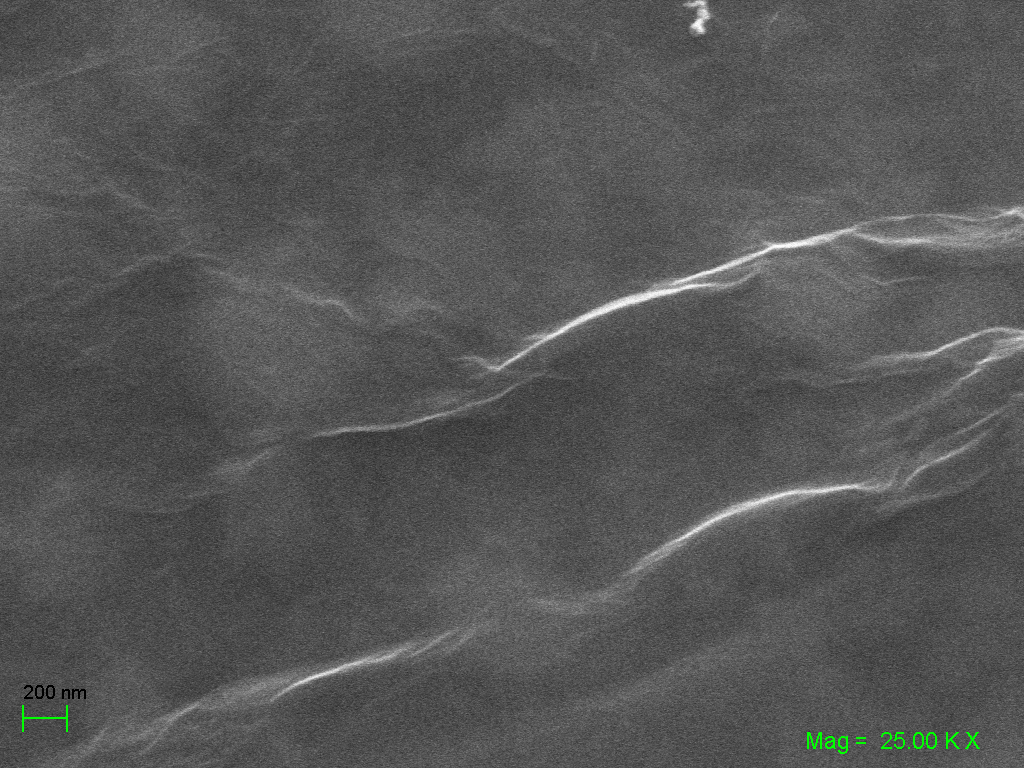
\includegraphics[width=\textwidth]{CRGO300517_paper.png}
			\end{subfigure}
			\begin{subfigure}{0.45\textwidth}
				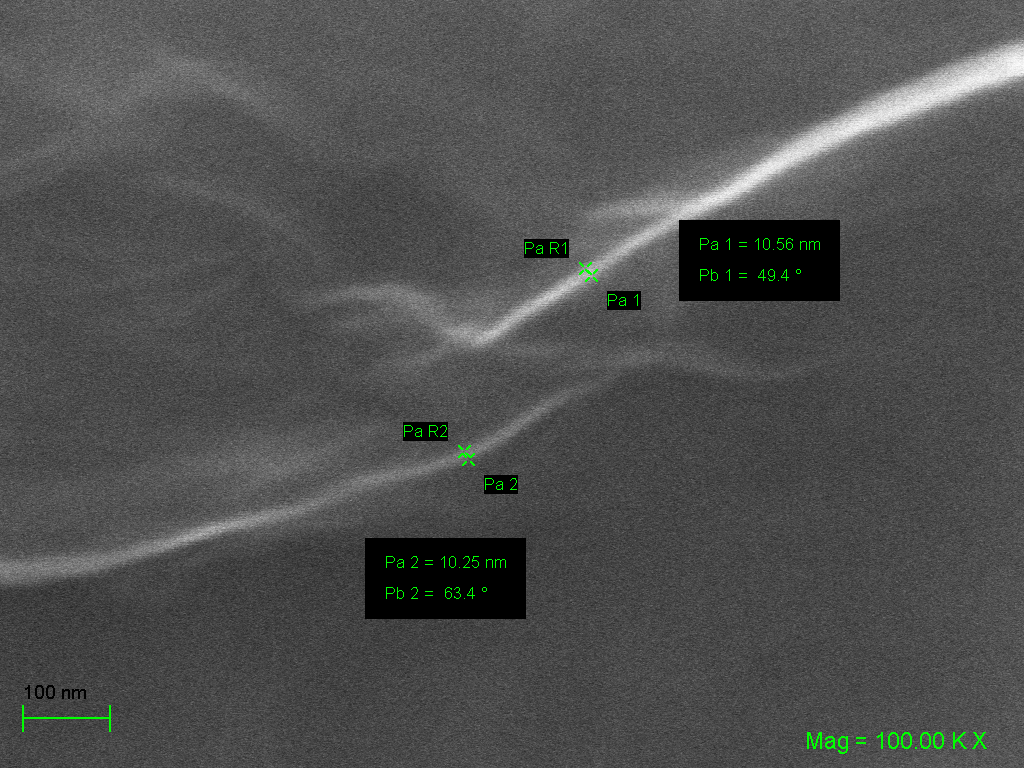
\includegraphics[width=\textwidth]{CRGO300517_paper_measures.png}
			\end{subfigure}
			\caption[Imagen SEM de un electrodo de rGO en formato papel]{Imagen SEM de un electrodo de rGO en formato papel.}
		\end{figure}
	\end{frame}


	\section{Supercondensadores}
	\begin{frame}[fragile]{Construcción de supercondensadores}
		\begin{figure}[h!]
			\begin{tikzpicture}[]
			\path[ use as bounding box] (-4,-2) rectangle(4,2);
				\only<1->{\begin{scope}
					\clip[] (-6.5, 0) rectangle (-2.5, 2.5);
					\node at (0,0) {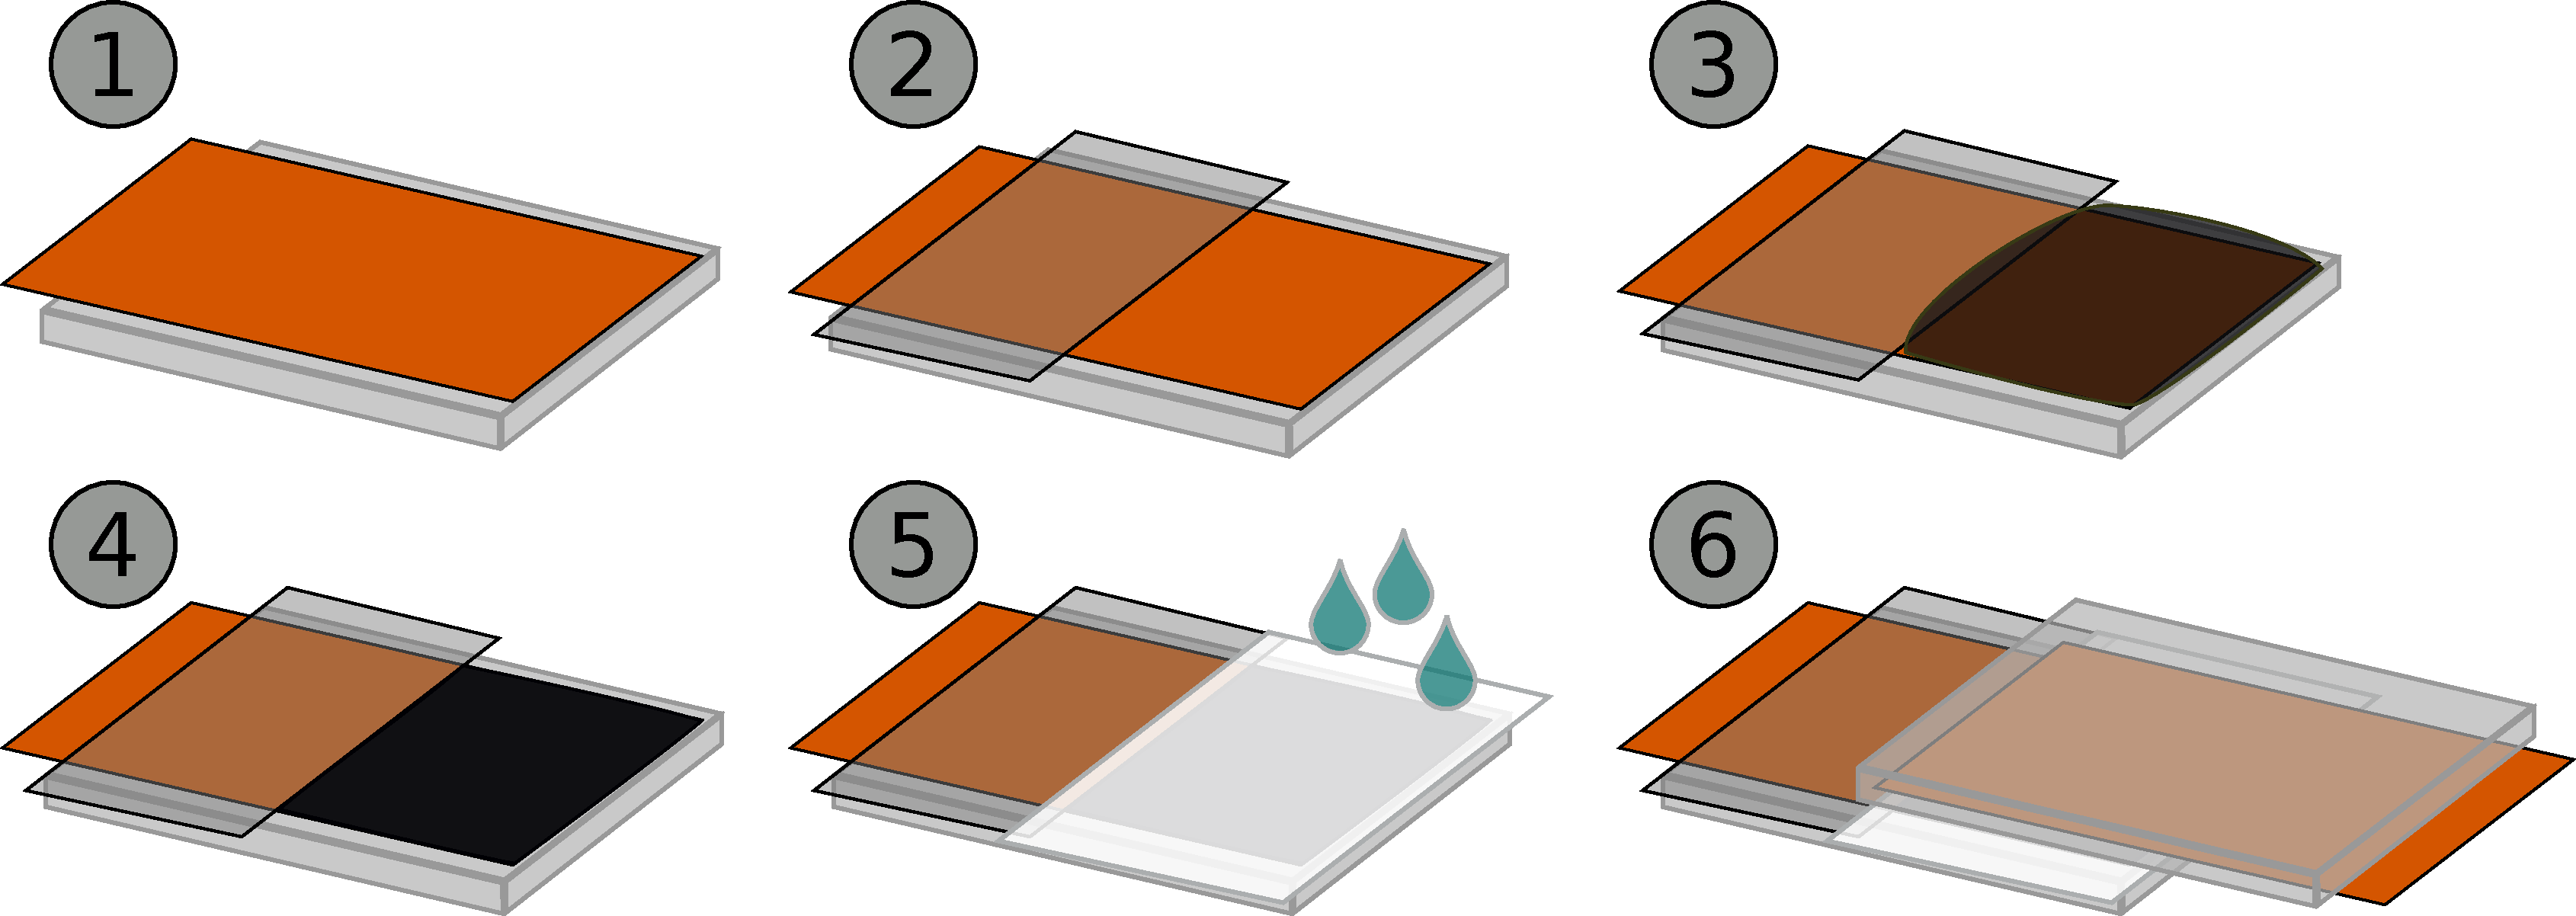
\includegraphics[width = 0.9\textwidth]{SC_process.pdf}};
				\end{scope}}
				\only<2->{\begin{scope}
					\clip[] (-2.5, 0) rectangle (1.5, 2.5);
					\node at (0,0) {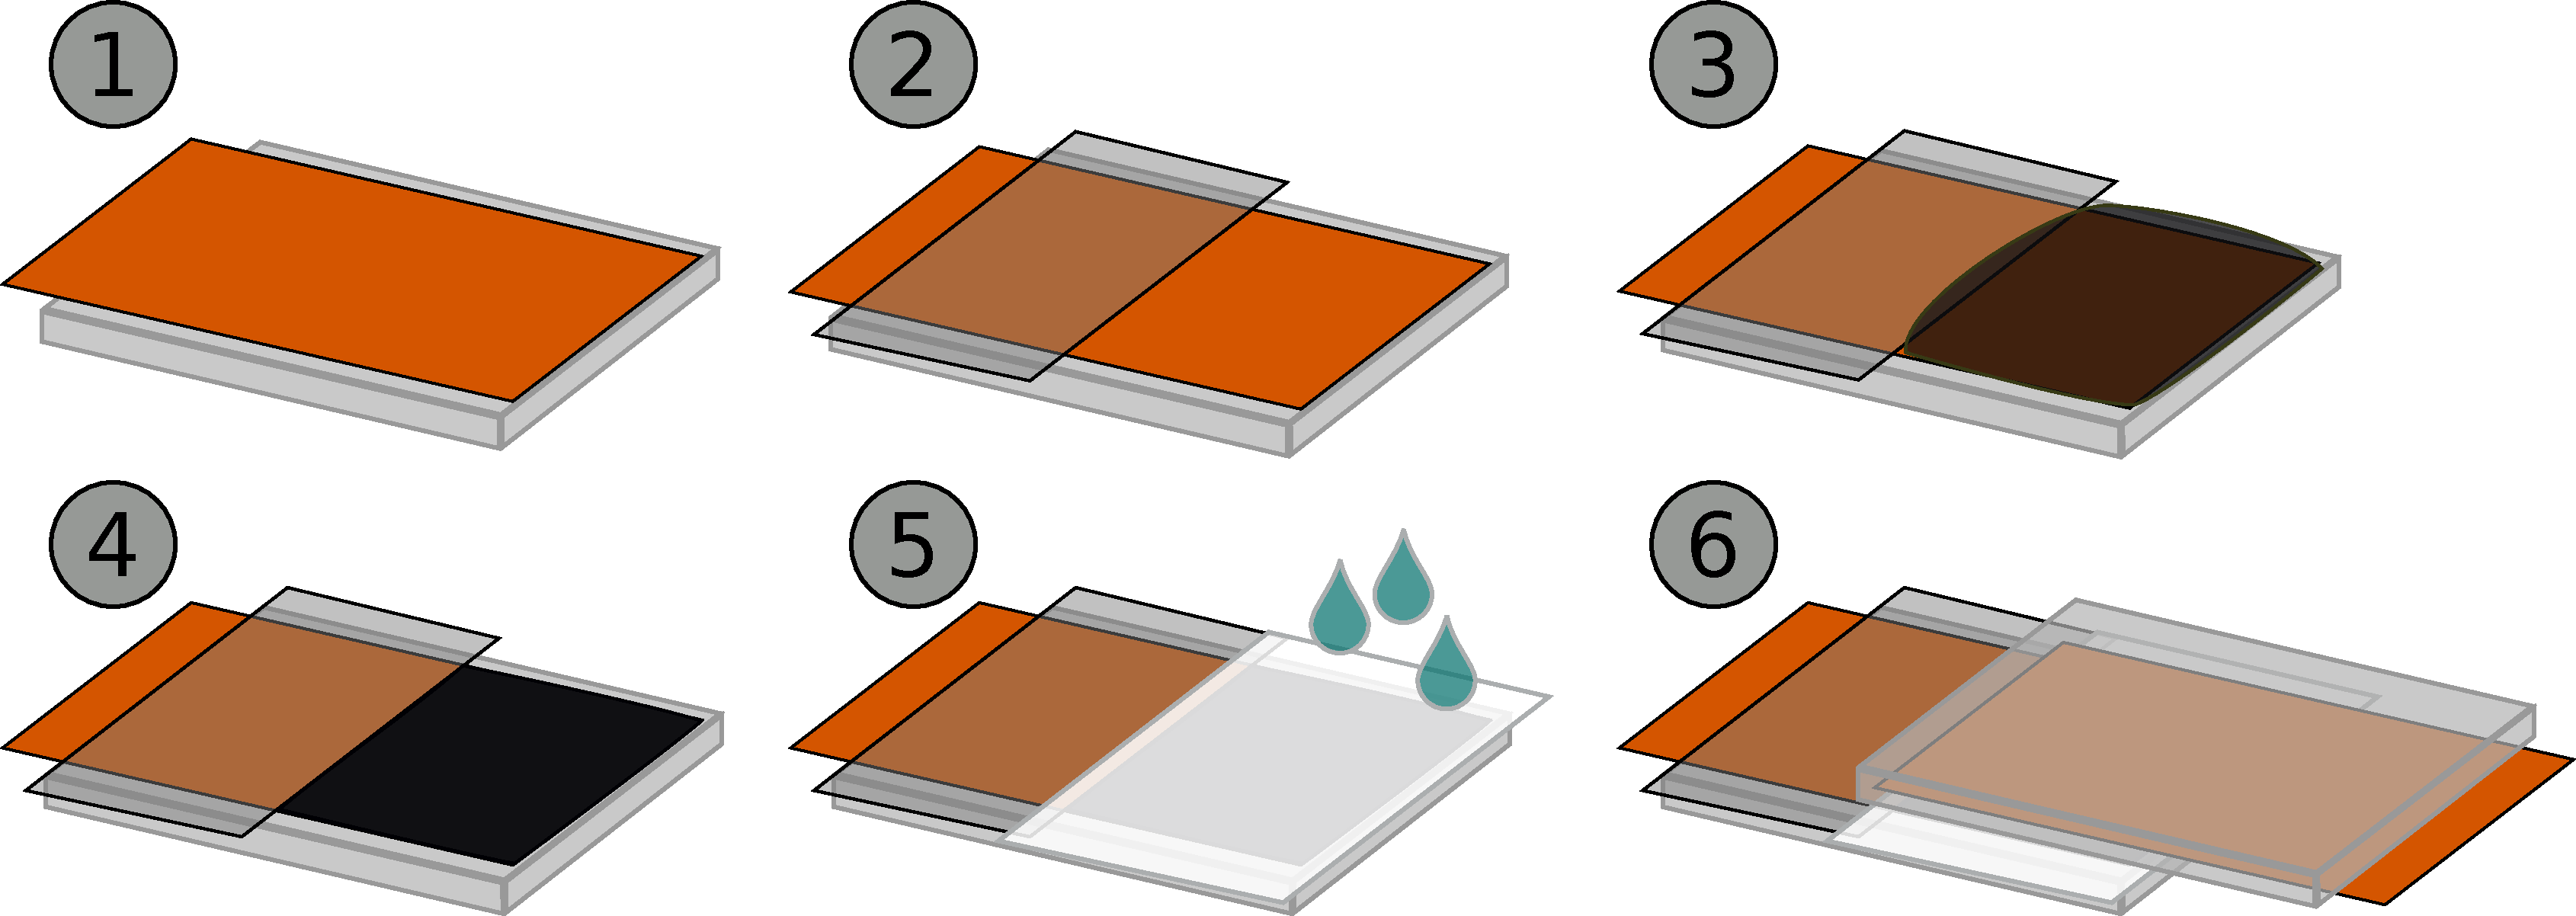
\includegraphics[width = 0.9\textwidth]{SC_process.pdf}};
				\end{scope}}
				\only<3->{\begin{scope}
					\clip[] (1.5, 0) rectangle (5.5, 2.5);
					\node at (0,0) {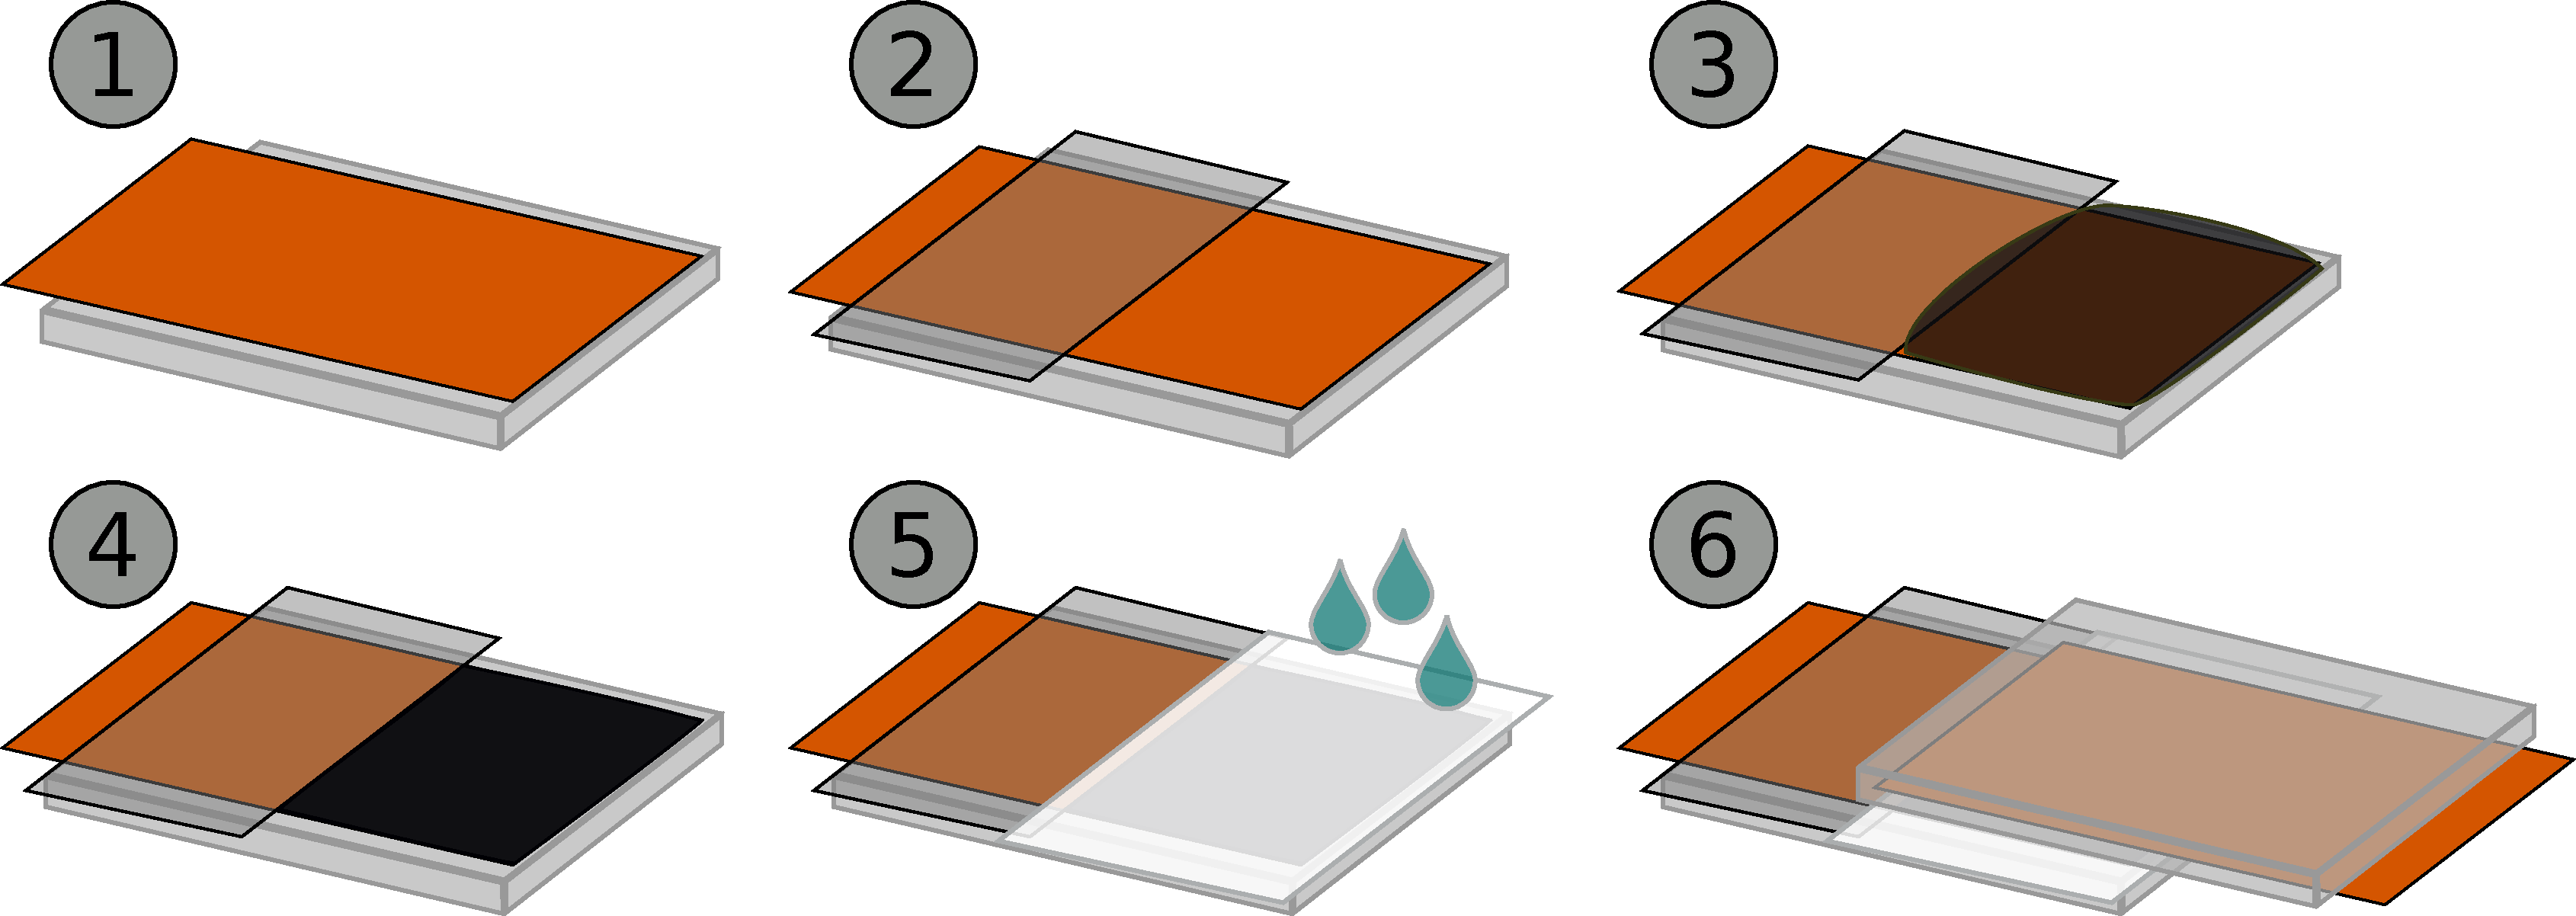
\includegraphics[width = 0.9\textwidth]{SC_process.pdf}};
				\end{scope}}
				\only<4->{\begin{scope}
					\clip[] (-6.5, 0) rectangle (-2.5, -2.5);
					\node at (0,0) {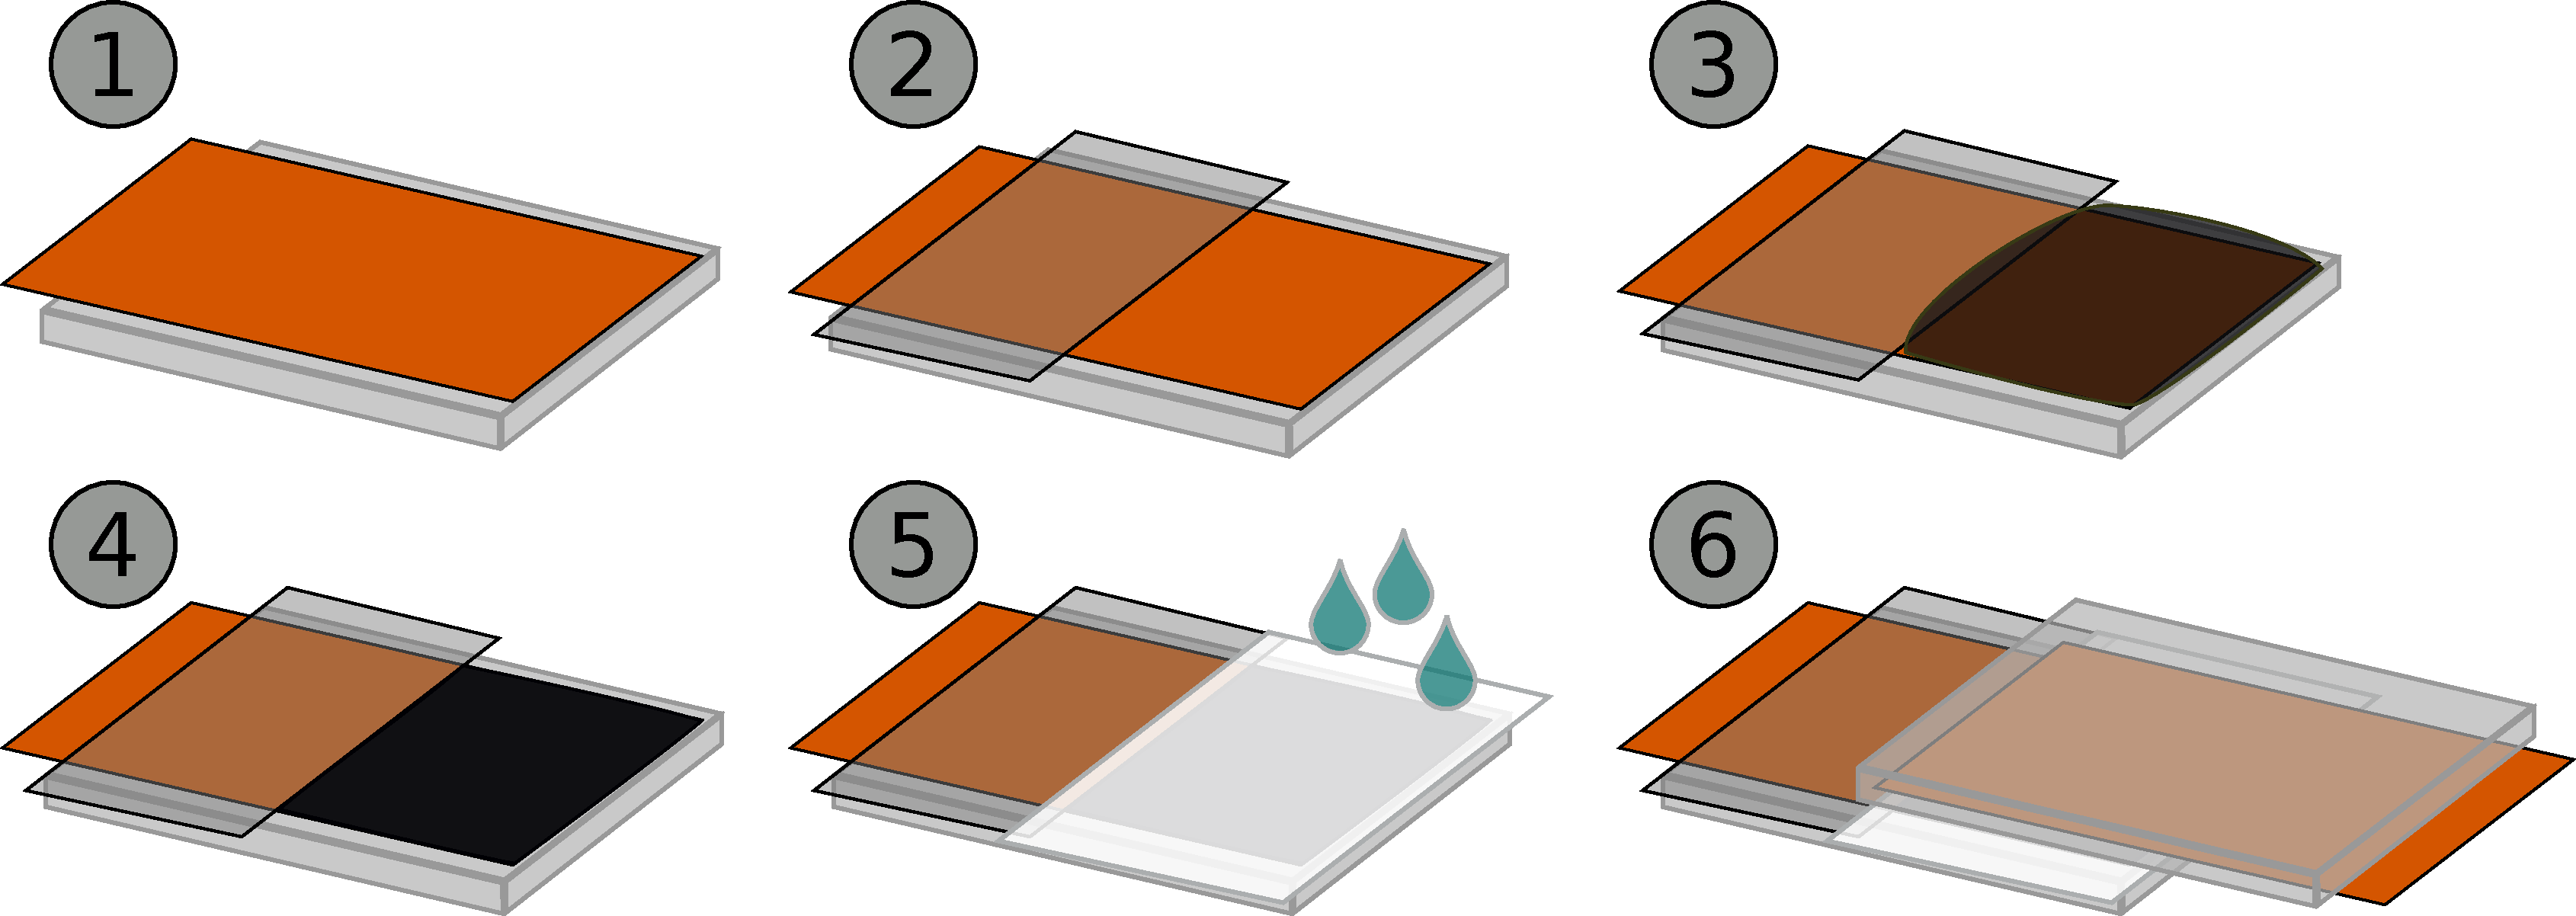
\includegraphics[width = 0.9\textwidth]{SC_process.pdf}};
				\end{scope}}
				\only<5->{\begin{scope}
					\clip[] (-2.5, 0) rectangle (1.5, -2.5);
					\node at (0,0) {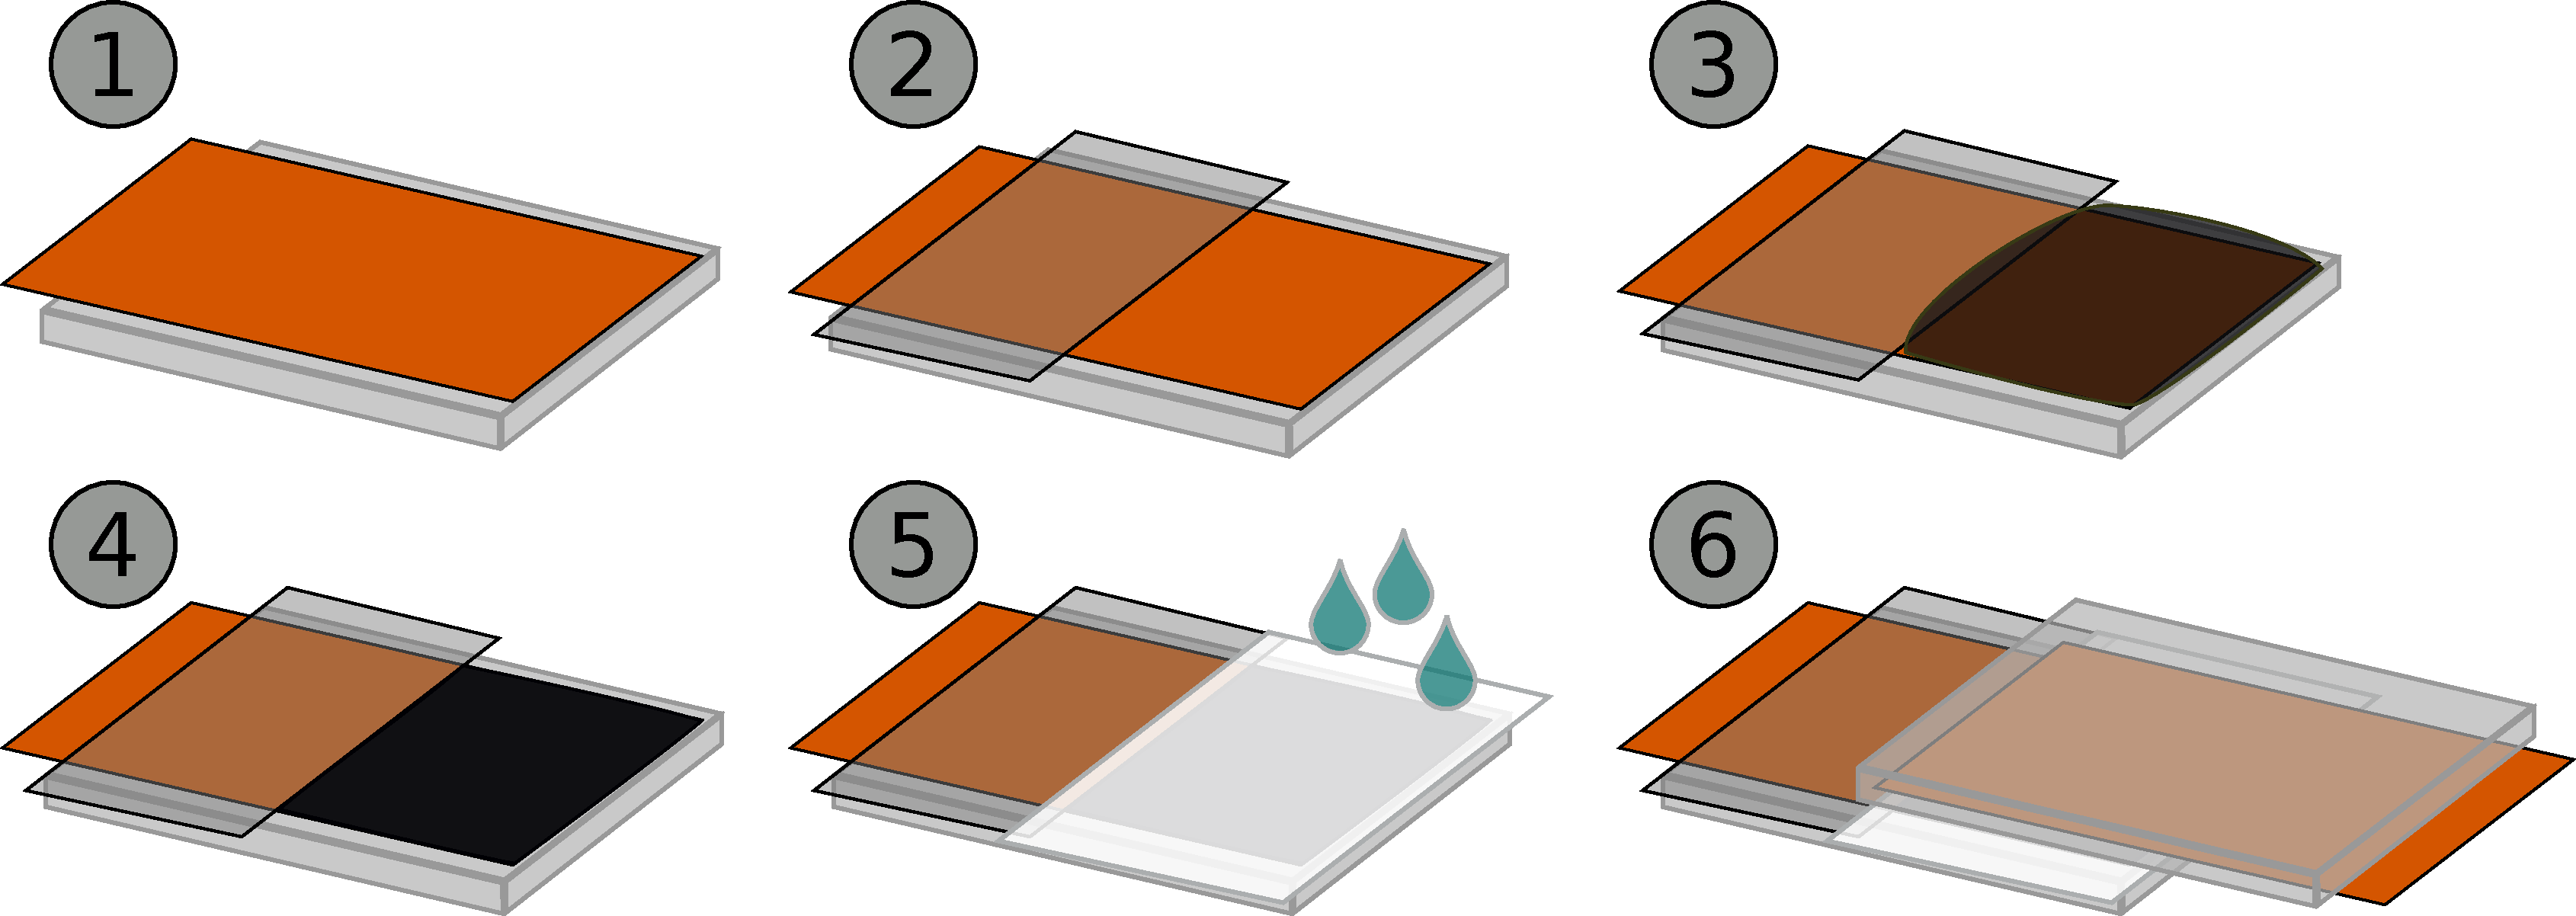
\includegraphics[width = 0.9\textwidth]{SC_process.pdf}};
				\end{scope}}
				\only<6->{\begin{scope}
					\clip[] (1.5, 0) rectangle (6.5, -2.5);
					\node at (0,0) {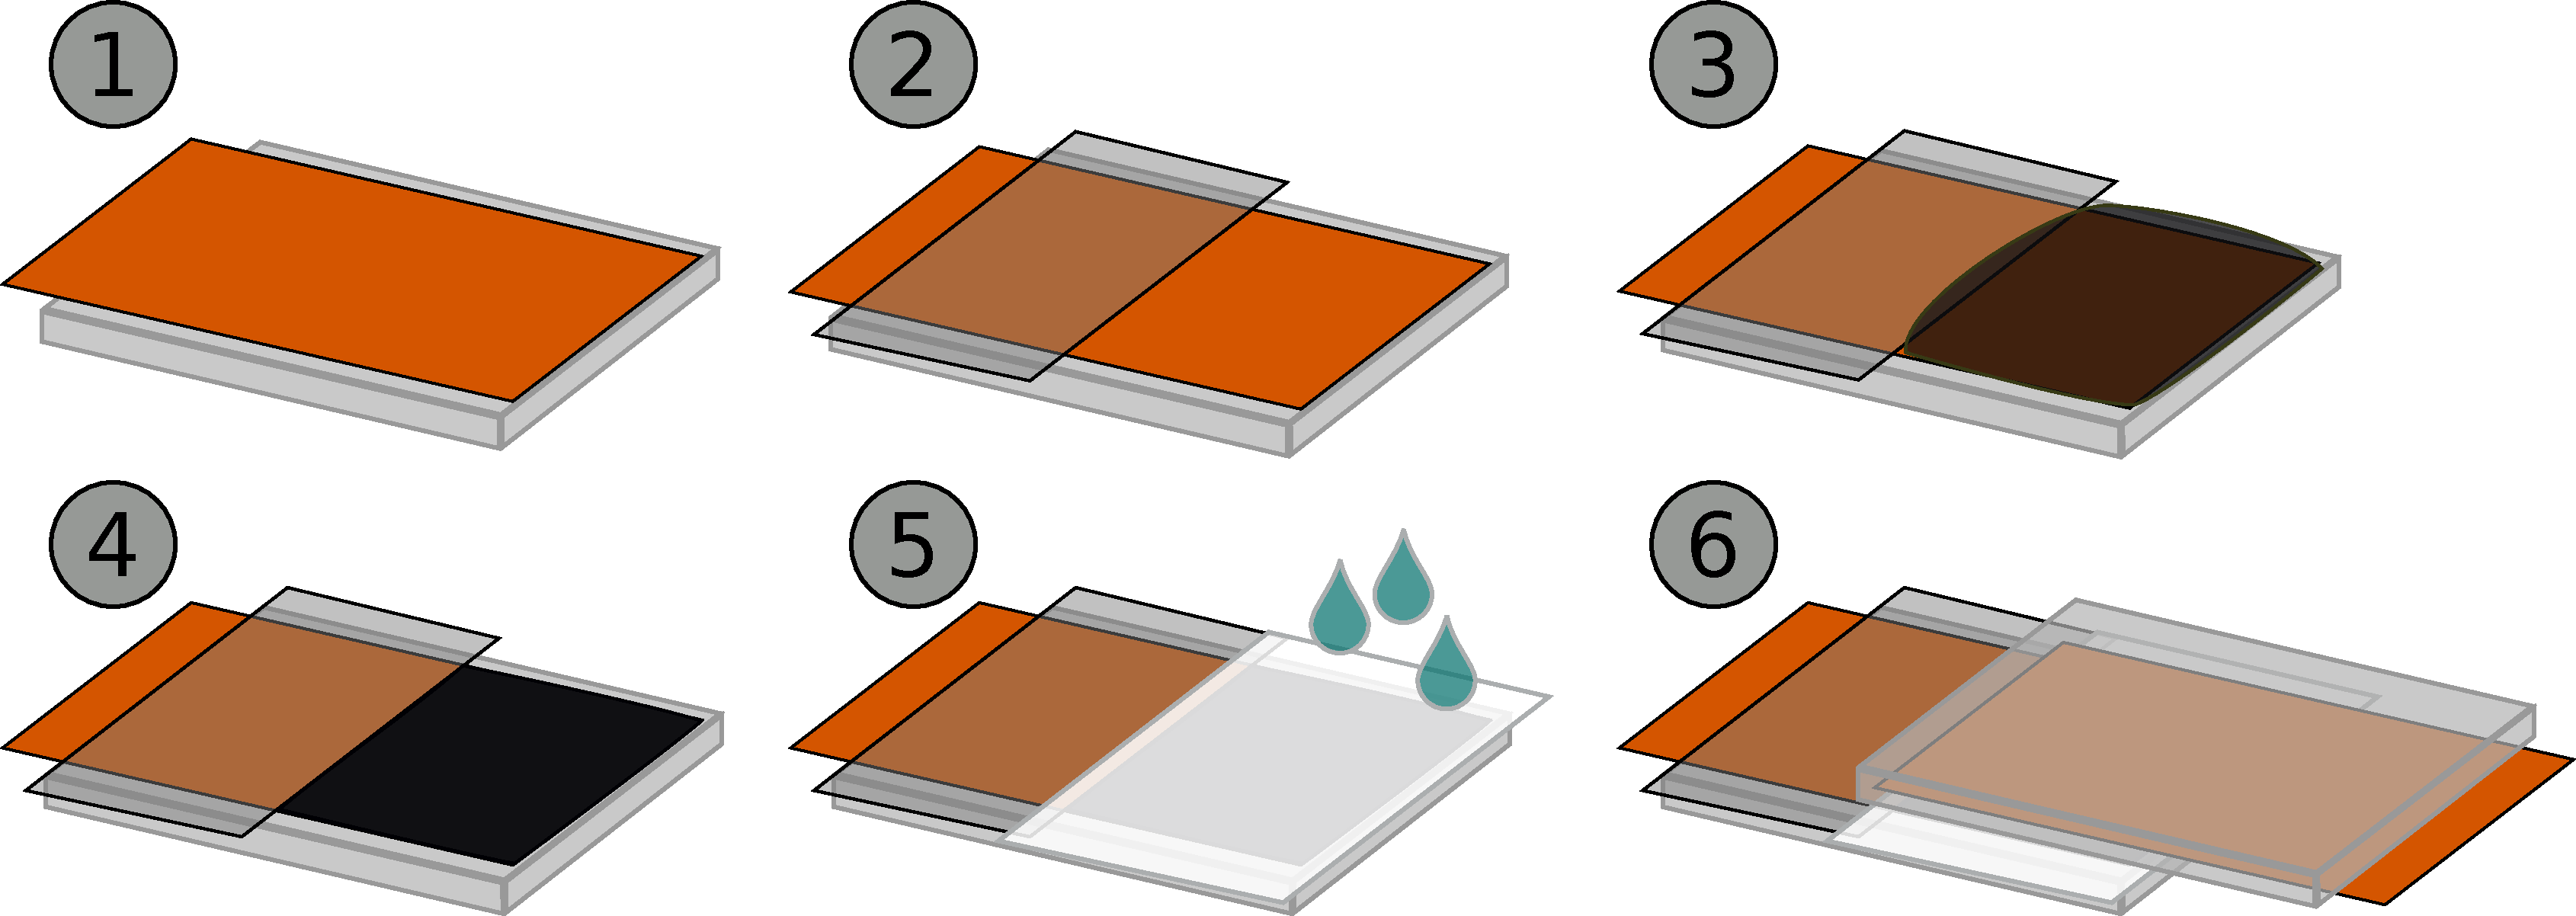
\includegraphics[width = 0.9\textwidth]{SC_process.pdf}};
				\end{scope}}
			\end{tikzpicture}
			\caption[Principio de contrucción de un supercondensador]{Secuencia para la construcción de un supercondensador básico.}
			\label{fig:SC_process}
		\end{figure}
	\end{frame}

	\begin{frame}{Construcción de supercondensadores}
		\only<1->\textbf{Problemas con la construcción de supercondensadores:}
		\begin{itemize}[<+(1)->]
			\item Los colectores de corriente de \textbf{aluminio} y \textbf{cobre} utilizados, \textbf{se degradan rápidamente}.
			\item La \textbf{deposición} de material en los colectores de corriente \textbf{no es homogénea}.
			\item El agua del electrolito se evapora rápidamente, \textbf{disminuyendo la cantidad de iones} en el medio de conducción. 
			\item El cierre del dispositivo \textbf{no es estable y no permite su reproducibilidad}.
			\item La conexión a los terminales eléctricos \textbf{no es estable}.
			\item[] \color{red} {\large \textbf{¡Hay que buscar otro método!}}
		\end{itemize}
	\end{frame}


	\begin{frame}{Celda de pruebas}
		\begin{columns}
			\begin{column}{0.5\textwidth}
				\textbf{Se decide diseñar una celda de pruebas}
				\begin{itemize}[<+->]
					\item Fácil manipulación.
					\item \textbf{Resistente a la corrosión.}
					\item \textbf{Hermético.}
					\item  \textbf{Reproducible}.
				\end{itemize}
			\end{column}
			\begin{column}{0.5\textwidth}
				\begin{figure}
					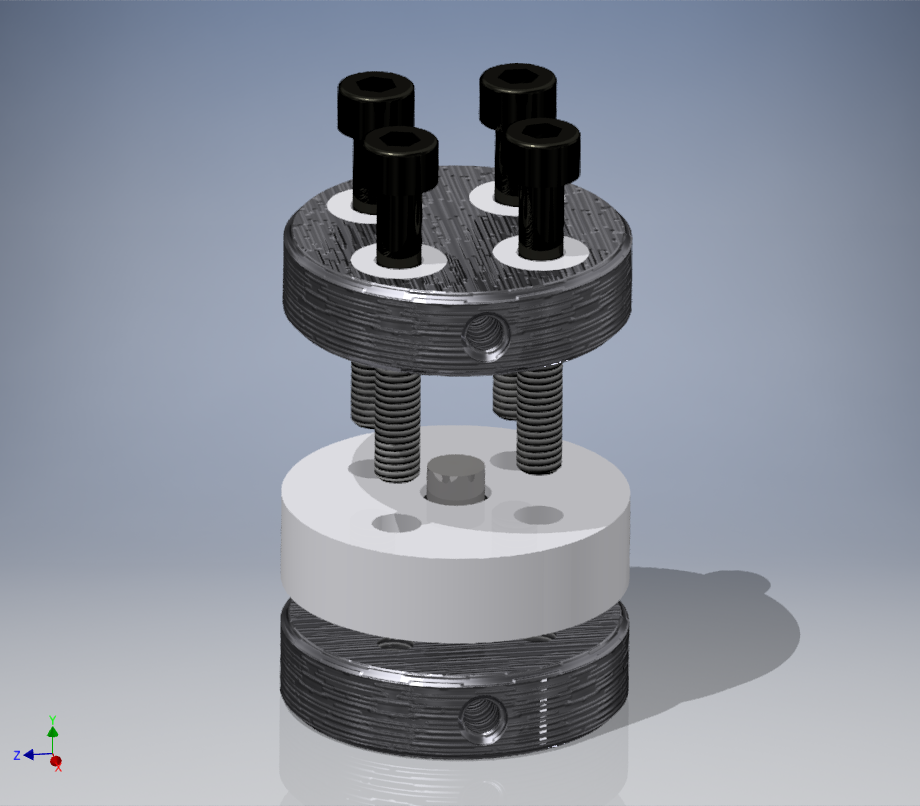
\includegraphics[width=\textwidth]{cell4.png}
				\end{figure}
			\end{column}
		\end{columns}
	\end{frame}


	\begin{frame}{Celda de pruebas}
		\begin{figure}[h!]
			\centering
			{
				\begin{subfigure}[b]{0.6\textwidth}
					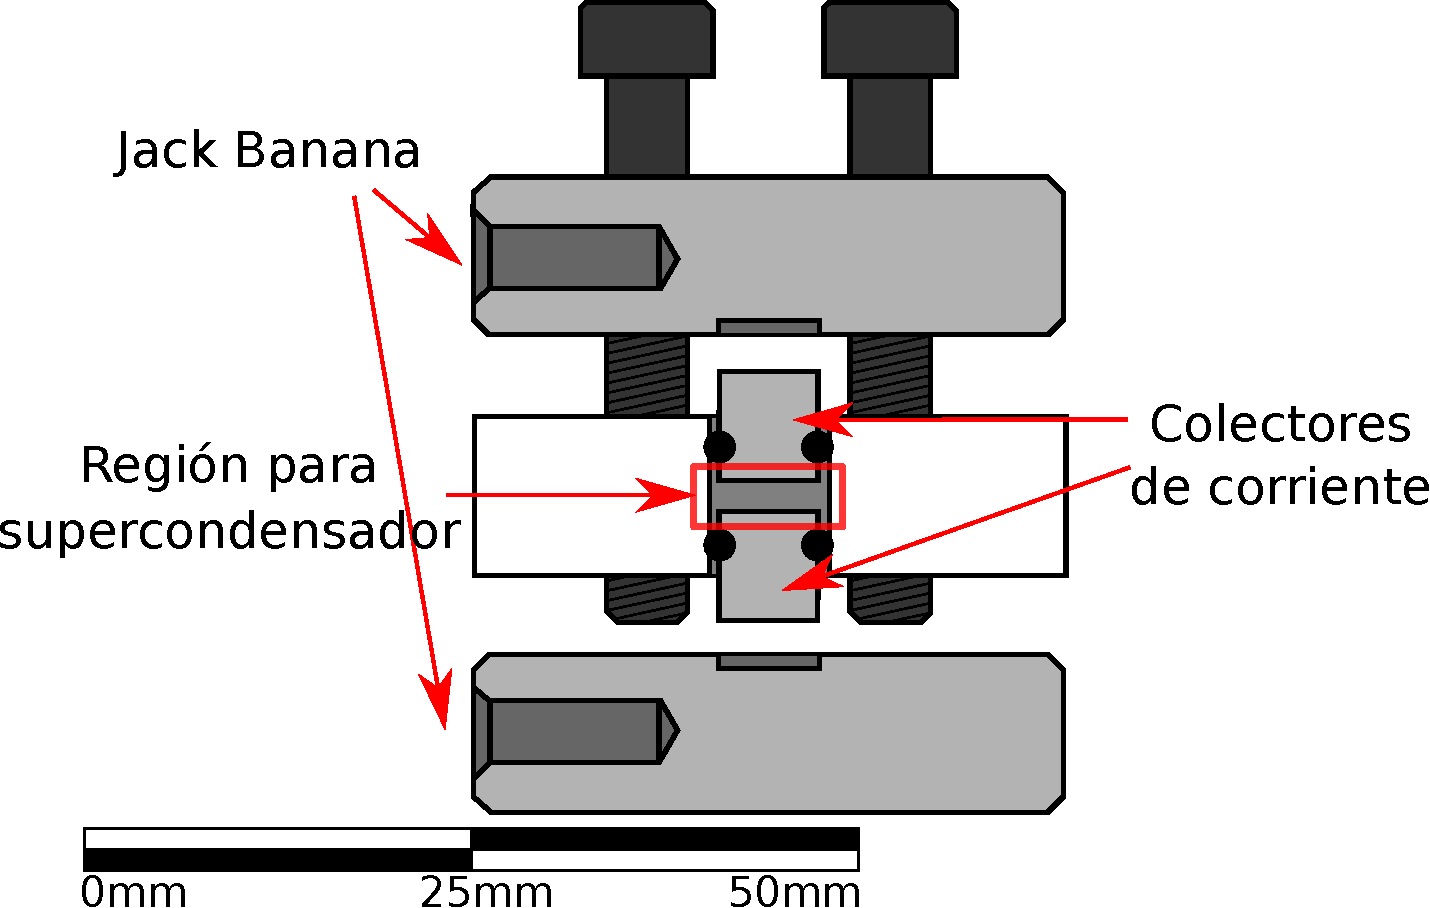
\includegraphics[width=\textwidth]{cell_scheme.pdf}
					\caption{}
					\label{fig:cell_scheme}
				\end{subfigure}\hfill
				\begin{subfigure}[b]{0.25\textwidth}
					\includegraphics[width=\textwidth]{cell_image.pdf}
					\caption{}
					\label{fig:cell_image}
				\end{subfigure}
			}
			\caption[Celda de pruebas de supercondensador]{\subref{fig:cell_scheme} vista en corte longitudinal de la celda de pruebas mostrando los componentes más importantes. \subref{fig:cell_image} fotografía de la celda armada y conectada al potenciostato.}
			\label{fig:celda_de_pruebas_SC}
		\end{figure}
	\end{frame}
	
	\newcommand{\electrodesWidth}{0.5\textwidth}
%	\begin{frame}{Construcción de electrodos}
%		\begin{figure}
%			\centering
%			\begin{adjustbox}{minipage=0.8\linewidth,frame}
%				\centering
%				\uncover<1->{\begin{subfigure}[b]{\electrodesWidth}
%					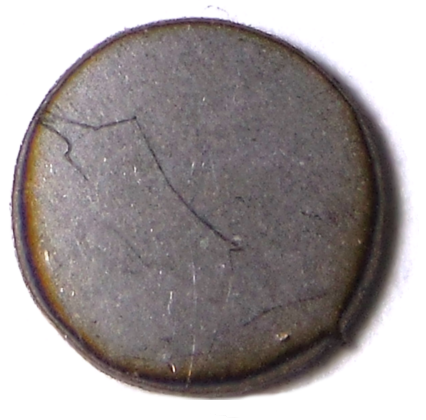
\includegraphics[width=\textwidth]{electrode_steel.png}
%					\caption{\mSustratoAcero}
%					\label{fig:substrate_steel}
%				\end{subfigure}}
%				\uncover<2->{\begin{subfigure}[b]{\electrodesWidth}
%					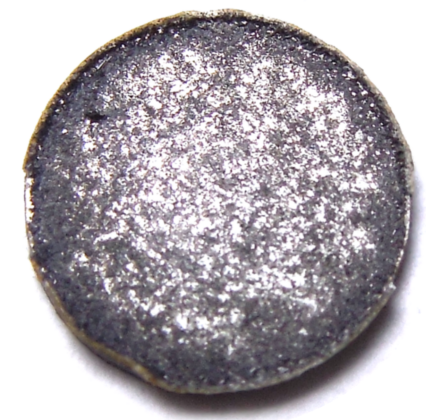
\includegraphics[width=\textwidth]{electrode_polvo_ac.png}
%					\caption{\mPolvoAcero}
%					\label{fig:electrode_powder_ac}
%				\end{subfigure}}
%				\uncover<3->{\begin{subfigure}[b]{\electrodesWidth}
%					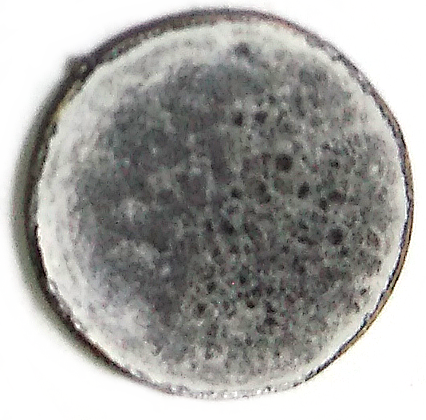
\includegraphics[width=\textwidth]{electrode_polvo_pmma_ac.png}
%					\caption{PolAc+pmma}
%					\label{fig:electrode_powder_pmma_z}
%				\end{subfigure}}
%				\uncover<4->{\begin{subfigure}[b]{\electrodesWidth}
%					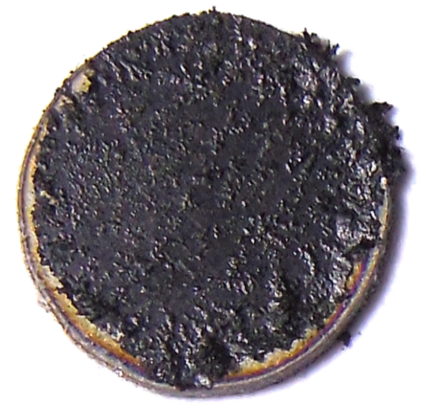
\includegraphics[width=\textwidth]{electrode_paper.png}
%					\caption{\mPapelAcero}
%					\label{fig:electrode_paper}
%				\end{subfigure}\linebreak}
%				\uncover<5->{\begin{subfigure}[b]{\electrodesWidth}
%					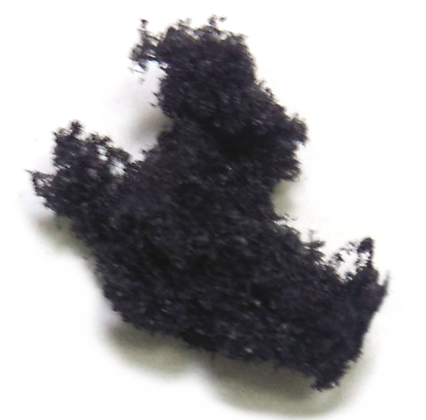
\includegraphics[width=\textwidth]{electrode_lio.png}
%					\caption{\mLiofilizadoAcero}
%					\label{fig:electrode_lio}
%				\end{subfigure}}
%				\uncover<6->{\begin{subfigure}[b]{\electrodesWidth}
%					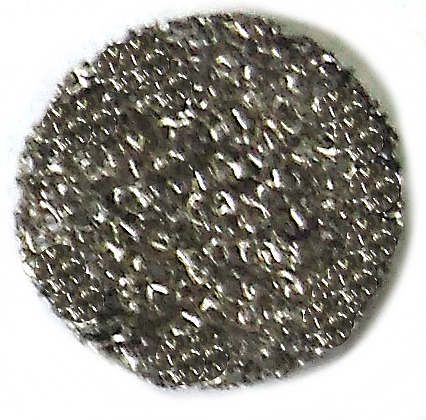
\includegraphics[width=\textwidth]{electrode_ni.png}
%					\caption{\mSustratoNiquel}
%					\label{fig:substrate_nickel}
%				\end{subfigure}}
%				\uncover<7->{\begin{subfigure}[b]{\electrodesWidth}
%					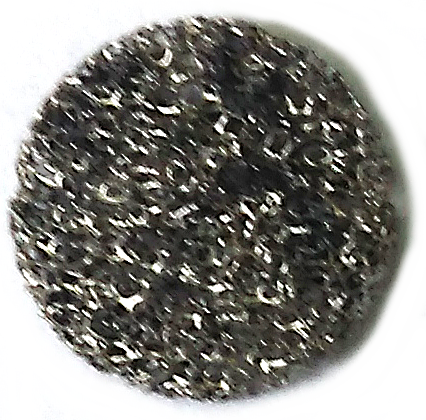
\includegraphics[width=\textwidth]{electrode_polvo_ni.png}
%					\caption{\mPolvoNiquel}
%					\label{fig:electrode_powder_ni}
%				\end{subfigure}}
%				\uncover<8->{\begin{subfigure}[b]{\electrodesWidth}
%					\includegraphics[width=\textwidth]{electrode_polvo_pmma_ni.png}
%					\caption{PolNi+pmma}
%					\label{fig:electrode_powder_pmma_ni}
%				\end{subfigure}}
%			\end{adjustbox}
%			\caption[Electrodos utilizados en la celda de pruebas de supercondensador]{Electrodos utilizados en la celda de pruebas de supercondensador.}
%			\label{fig:electrodes}
%		\end{figure}
%	\end{frame}

	\begin{frame}{Construcción de electrodos}
	\captionsetup[subfigure]{labelformat=empty}
		\begin{columns}
			\begin{column}{0.3\textwidth}
				\begin{figure}
					\uncover<1->{\begin{subfigure}[b]{\electrodesWidth}
						\includegraphics[width=\textwidth]{electrode_steel.png}
						\caption{\mSustratoAcero}
					\end{subfigure}}\\
					\uncover<3->{\begin{subfigure}[b]{\electrodesWidth}
						\includegraphics[width=\textwidth]{electrode_ni.png}
						\caption{\mSustratoNiquel}
					\end{subfigure}}
				\end{figure}
			\end{column}
			\begin{column}{0.6\textwidth}
				\textbf{Sustratos}
				\begin{itemize}[<+(1)->]
					\item Sustrato de \textbf{acero 316}.
					\item Sustrato de \textbf{espuma de níquel}.
					\item Diámetro de \textbf{7mm}.
				\end{itemize}
			\end{column}
		\end{columns}		
	\end{frame}

	\begin{frame}{Construcción de electrodos}
	\captionsetup[subfigure]{labelformat=empty}
		\begin{columns}
			\begin{column}{0.3\textwidth}
				\begin{figure}
					\uncover<1->{\begin{subfigure}[b]{\electrodesWidth}
						\includegraphics[width=\textwidth]{electrode_polvo_ac.png}
						\caption{\mPolvoAcero}
					\end{subfigure}}
					\uncover<4->{\begin{subfigure}[b]{\electrodesWidth}
						\includegraphics[width=\textwidth]{electrode_polvo_pmma_ac.png}
						\caption{PolAc+pmma}
					\end{subfigure}}
				\end{figure}
			\end{column}
			\begin{column}{0.6\textwidth}
				\textbf{Electrodos}
				\begin{itemize}[<+(1)->]
					\item Dispersión en \textbf{etilengilicol}, depositada por goteo, y evaporación del dispersante.
					\item[!] La deposición \textbf{no es homogénea}.
					\item Dispersión en \textbf{solución de pmma en acetona}, depositada por goteo, y evaporación del solvente.
					\item[!] \textbf{Mucho aglutinante}.
				\end{itemize}
			\end{column}
		\end{columns}		
	\end{frame}

	\begin{frame}{Construcción de electrodos}
	\captionsetup[subfigure]{labelformat=empty}
		\begin{columns}
			\begin{column}{0.3\textwidth}
				\begin{figure}
					\uncover<1->{\begin{subfigure}[b]{\electrodesWidth}
						\includegraphics[width=\textwidth]{electrode_paper.png}
						\caption{\mPapelAcero}
					\end{subfigure}\linebreak}
					\uncover<4->{\begin{subfigure}[b]{\electrodesWidth}
						\includegraphics[width=\textwidth]{electrode_lio.png}
						\caption{\mLiofilizadoAcero}
					\end{subfigure}}
				\end{figure}
			\end{column}
			\begin{column}{0.6\textwidth}
				\textbf{Electrodos}
				\begin{itemize}[<+(1)->]
					\item Lámina parecida al \textbf{papel}.
					\item[!] Bordes irregulares.
					\item Material \textbf{liofilizado}.
					\item[!] Desconocimiento del resultado.
				\end{itemize}
			\end{column}
		\end{columns}		
	\end{frame}

	\begin{frame}{Construcción de electrodos}
	\captionsetup[subfigure]{labelformat=empty}
		\begin{columns}
			\begin{column}{0.3\textwidth}
				\begin{figure}
					\uncover<1->{\begin{subfigure}[b]{\electrodesWidth}
						\includegraphics[width=\textwidth]{electrode_polvo_ni.png}
						\caption{\mPolvoNiquel}
					\end{subfigure}}
					\uncover<4->{\begin{subfigure}[b]{\electrodesWidth}
						\includegraphics[width=\textwidth]{electrode_polvo_pmma_ni.png}
						\caption{PolNi+pmma}
					\end{subfigure}}
				\end{figure}
			\end{column}
			\begin{column}{0.6\textwidth}
				\textbf{Electrodos}
				\begin{itemize}[<+(1)->]
					\item Dispersión en \textbf{etilenglicol}, deposición por goteo, y evaporación del dispersante.
					\item[!] La dispersión \textbf{escurre fuera del electrodo}.
					\item Dispersión en \textbf{solución de ppma en acetona}, deposición por goteo, y evaporación del solvente.
					\item[!] La dispersión \textbf{escurre fuera del electrodo}.
				\end{itemize}
			\end{column}
		\end{columns}		
	\end{frame}

	\begin{frame}{Resumen electrodos}
		\begin{tabular}{l|c|c|c|c|c|c}
			&
			\includegraphics[width=0.08\textwidth]{electrode_polvo_ac.png} & \includegraphics[width=0.08\textwidth]{electrode_polvo_pmma_ac.png} & \includegraphics[width=0.08\textwidth]{electrode_paper.png} & \includegraphics[width=0.08\textwidth]{electrode_lio.png} & \includegraphics[width=0.08\textwidth]{electrode_polvo_ni.png} & \includegraphics[width=0.08\textwidth]{electrode_polvo_pmma_ni.png} \\
			\hline
			Nombre & PolvoAc & PolvoAc+ & PapelAc & LioAc & PolvoNi & PolvoNi\\
					&		& pmma		&			&				&	pmma\\
			\hline
			Masa [mg] & 0,4 $\pm$ 0,2 & 2,8 $\pm$ 0,2 & 0,6 $\pm$ 0,1 & 0,6 $\pm$ 0,1 & 0,9 $\pm$ 0,2 & 0,8 $\pm$ 0,2
			

		\end{tabular}
	\end{frame}
	
%	\begin{frame}[fragile]{Caracterización electroquímica}
%		\begin{figure}
%			\begin{tikzpicture}
%				[scale=1,trim axis right,trim axis left]
%				\begin{axis}
%				[
%				CVStyle,
%				domain=-1:1,
%				legend entries={Ideal, Real},				
%				]
%	 		 	\addplot[green!60!black, thick] table {
%	 		 		A B
%	 		 		-1  1
%	 		 		 1  1
%	 		 		
%	 		 		 1 -1
%	 		 		-1 -1
%	 		 	};
% 		 		\addplot[green!60!black, thick, dashed, forget plot] table {
% 		 			A B
% 		 			-1 -1
% 		 			-1  1
% 		 			
% 		 			1  1
% 		 			1 -1
% 		 		};
% 	 			\addplot[thick,color=red, smooth,samples=100,domain=0:0.4] plot[parametric] function{1.57041*t**(3)+0*t**(2)+0.4621*t-1,-0.11402*t**(3)+0*t**(2)+3.25798*t-1};
% 	 			\addplot[thick,color=red, smooth,samples=100,domain=0.4:0.54] plot[parametric] function{8.70966*t**(3)-8.49528*t**(2)+3.83173*t-1.44552,-14.95269*t**(3)+17.65714*t**(2)-3.74567*t-0.07401};
% 	 			\addplot[thick,color=red, smooth,samples=100,domain=0.54:0.8] plot[parametric] function{-8.63754*t**(3)+19.61633*t**(2)-11.35349*t+1.28871,7.29314*t**(3)-18.39283*t**(2)+15.72766*t-3.58035};
% 	 			\addplot[thick,color=red, smooth,samples=100,domain=0.80:1.0] plot[parametric] function{1.73159*t**(3)-5.19477*t**(2)+8.43573*t-3.97255,1.55121*t**(3)-4.65363*t**(2)+4.76933*t-0.66691};
%				
%				\addplot[thick, red, smooth, samples=100,domain=0:0.4] plot[parametric] function{-1.57041*t**(3)+0*t**(2)-0.4621*t+1,0.11402*t**(3)+0*t**(2)-3.25798*t+1};
%				\addplot[thick, red, smooth, samples=100,domain=0.4:0.54] plot[parametric] function{-8.70966*t**(3)+8.49528*t**(2)-3.83173*t+1.44552,14.95269*t**(3)-17.65714*t**(2)+3.74567*t+0.07401};
%				\addplot[thick, red, smooth, samples=100,domain=0.54:0.8] plot[parametric] function{8.63754*t**(3)-19.61633*t**(2)+11.35349*t-1.28871,-7.29314*t**(3)+18.39283*t**(2)-15.72766*t+3.58035};
%				\addplot[thick, red, smooth, samples=100,domain=0.80:1.0] plot[parametric] function{-1.73159*t**(3)+5.19477*t**(2)-8.43573*t+3.97255,-1.55121*t**(3)+4.65363*t**(2)-4.76933*t+0.66691};
% 		 		\end{axis}
%			\end{tikzpicture}
%		\end{figure}
%	\end{frame}
%
%	\begin{frame}{Caracterización electroquímica}
%		\begin{table}[h!]
%			\centering
%			\begin{tabular}{ l r }
%				Voltametría cíclica &  \\
%				\hline
%				Voltaje inicial [V] & 0 \\
%				Límite inferior [V] & -0,8 \\
%				Límite superior [V] & 0,8  \\
%				Número de ciclos & 3 \\
%				Velocidad de barrido [mV/s] & 25, 50, 100, 200, 400
%			\end{tabular}
%		\end{table}
%	\end{frame}
%
%	\begin{frame}[fragile]{Caracterización electroquímica}
%		\begin{figure}
%			\begin{tikzpicture}
%			[scale=1,trim axis right,trim axis left]
%			\begin{axis}
%			[
%			CCDStyle,
%			legend entries={Ideal, Real}			
%			]
%			\addplot[green!60!black, thick] table {
%				A B
%				0 0
%				1 1
%				2 0
%			};
%			\addplot[red, thick, domain=0:1] (\x,{-0.8*(\x)^(2)+1.6*(\x)+0.2});
%			\addplot[red, thick, domain=1:2] (\x,{0.8*(\x)^(2)-3.2*(\x)+3.2});
%			\addplot[red, thick, dashed] table {
%				A B
%				0 0
%				0 0.2
%			
%				1 1
%				1 0.8
%			};
%			\end{axis}
%			\end{tikzpicture}
%		\end{figure}
%	\end{frame}
%
%	\begin{frame}{Caracterización electroquímica}
%\begin{table}[h!]
%	\centering
%	\begin{tabular}{ l r }
%		Carga y descarga cíclica & \\
%		\hline
%		Densidad de corriente [A/g] & 0,1 ó 	1 \\
%		Número de ciclos & 1000 \\
%		Límite inferior [V] & 0 \\
%		Límite superior [V] & 1 \\
%	\end{tabular}
%	\label{tab:elec_config}
%	\caption[Parámetros de cada medición electroquímica]{Parámetros de cada medición electroquímica.}
%\end{table}
%\end{frame}
%
%	\begin{frame}{Caracterización electroquímica}
%\begin{table}[h!]
%	\centering
%	\begin{tabular}{ l r }
%		Espectroscopía de impedancia electroqúimica & \\
%		\hline
%		Frecuencia inicial	&	1 MHz \\
%		Frecuencia final	&	0.1 Hz \\
%		Corriente de exitación & 1 mA rms \\ 
%	\end{tabular}
%\end{table}
%\end{frame}

	\begin{frame}[fragile]{Metodología de medición}
		\textbf{¿Cómo se lleva a cabo la caracterización?}
		\begin{enumerate}[<+(1)->]
			\item Voltametría cíclica.
			\item Espectroscopia de impedancia.
			\item Carga y descaga cíclica.
			\item Voltametría cíclica.
		\end{enumerate}
	\end{frame}

	\begin{frame}{Resultados: Voltametría cíclica}
		\begin{figure}[h!]
			\centering
			\hfill
			\begin{subfigure}[b]{0.4\textwidth}
				\begin{tikzpicture}[scale=\plotscale, trim axis right,trim axis left]
				\begin{axis}
				[
				CVStyle,
				legend entries={\mPapelAcero, \mLiofilizadoAcero}
				]
				\addplot table [x=Voltaje, y expr=\thisrow{Corriente}/0.0006 ] {./Data/CV_CRGO300517_11/raw/sample3.txt};
				\addplot table [x=Voltaje, y expr=\thisrow{Corriente}/0.0006 ] {./Data/CV_CRGO300517_13/raw/sample3.txt};
				\end{axis}
				\end{tikzpicture}
%				\subcaption{Antes de 1000 ciclos de carga y descarga.}
			\end{subfigure}\hfill
			\begin{subfigure}[b]{0.4\textwidth}
				\begin{tikzpicture}[scale=\plotscale, trim axis right,trim axis left]
				\begin{axis}[
				CVStyle,
				legend entries={\mPolvoAcero, \mPolvoAceroPMMA, \mPolvoNiquel, \mPolvoNiquelPMMA},
				cycle list shift=2
				]
				\addplot table [x=Voltaje, y expr=\thisrow{Corriente}/0.0004 ] {./Data/CV_CRGO300517_9/raw/sample3.txt};
				\addplot table [x=Voltaje, y expr=\thisrow{Corriente}/0.0028 ] {./Data/CV_CRGO300517_3/raw/sample3.txt};
				\addplot table [x=Voltaje, y expr=\thisrow{Corriente}/0.0009 ] {./Data/CV_CRGO300517_5/raw/sample3.txt};
				\addplot table [x=Voltaje, y expr=\thisrow{Corriente}/0.0008 ] {./Data/CV_CRGO300517_7/raw/sample3.txt};	
				\end{axis}
				\end{tikzpicture}
%				\subcaption{Antes de 1000 ciclos de carga y descarga.}
			\end{subfigure}
			\caption{Resumen voltametría cíclica a 100 mV/s antes de 1000 ciclos de carga y descarga. Las muestras son separadas en dos gráficos para mejorar su visualización.}
		\end{figure}
	\end{frame}


	\begin{frame}{Resultados: Voltametría cíclica}
		\begin{table}[h!]
			\centering
			\begin{tabular}{ l l c c c }
				\multirow{2}{*}{Muestra}& \multirow{2}{*}{Masa [mg]}& \multirow{2}{*}{Capacitancia [mF]}	& Capacitancia & \multirow{2}{*}{Error}\\
				&         			      & 										& específica [F/g]     &			\\
				\hline
				\mSustratoAcero		&  -            &			0.1			&	-				&	-		\\
				\mPolvoAcero		& 0,4 $\pm$ 0,2 &			1.2			&	3.0	$\pm$ 1.5	&	50\%	\\
				\mPolvoAceroPMMA	& 2,8 $\pm$ 0,2 &			0.78		&	0.28 $\pm$ 0.02	&	7\%		\\
				\rowcolor{samplegreen}
				\mPapelAcero		& 0,6 $\pm$ 0,1 &			16.8		&	28.0 $\pm$ 4.7	&	17\%	\\
				\rowcolor{samplegreen}
				\mLiofilizadoAcero	& 0,6 $\pm$ 0,1 &			19.9		&	33.2 $\pm$ 5.5	&	17\%	\\
				\mSustratoNiquel	&    -          &			0.1			&	- 				&	-		\\
				\mPolvoNiquel		& 0,9 $\pm$ 0,2 &			0.3			&	0.35 $\pm$ 0.07	&	20\%	\\
				\mPolvoNiquelPMMA	& 0,8 $\pm$ 0,2 &			1.2			&	1.5	$\pm$ 0.4	&	27\%	\\
			\end{tabular}                                                          
			\label{tab:resumen_capacitancia}
			\caption{Resumen de capacitancia y capacitancia específica a 100 mV/s.}
		\end{table}
	\end{frame}

	\begin{frame}{Resultados: Espectro de impedancia electroquímica}
		\begin{figure}[h!]
			\centering
			\hfill
			\begin{subfigure}[b]{0.4\textwidth}
				\begin{tikzpicture}[scale=\plotscale,trim axis right,trim axis left]
				\begin{axis}[
				EISStyle,
				every axis legend/.append style={
					font=\normalsize,
					at={(0.02,0.98)},
					anchor=north west,
				},
				legend entries = {\mPapelAcero, \mLiofilizadoAcero}
				]
				\pgfplotstableread{./Data/CV_CRGO300517_11/raw/eisgalv.txt}{\eistable};
				\pgfplotstablegetrowsof{\eistable}
				\pgfmathsetmacro{\N}{\pgfplotsretval}
				\addplot table [only marks, x=Zreal, y expr=\thisrow{Zimag}*-1] {\eistable}
				node[pos=(1-1)/(\N-1), pin=right:{1 MHz}]{}
				node[pos=(\N-1)/(\N-1), pin=left:{0,1 Hz}]{};
				\pgfplotstableread{./Data/CV_CRGO300517_13/raw/eisgalv.txt}{\eistable};
				\pgfplotstablegetrowsof{\eistable}
				\addplot table [only marks, x=Zreal, y expr=\thisrow{Zimag}*-1] {\eistable}
				node[pos=(1-1)/(\N-1), pin=right:{1 MHz}]{}
				node[pos=(40-1)/(\N-1), ]{}
				node[pos=(\N-1)/(\N-1), pin=left:{0,1 Hz}]{};
				\end{axis}
				\end{tikzpicture}
			\end{subfigure}\hfill
			\begin{subfigure}[b]{0.4\textwidth}
				\begin{tikzpicture}[scale=\plotscale,trim axis right,trim axis left]
				\begin{axis}[
				EISStyle,
				every axis legend/.append style={
					font=\normalsize,
					at={(0.98,0.02)},
					anchor=south east,
				},
				legend entries = {\mPolvoAcero, \mPolvoAceroPMMA, \mPolvoNiquel, \mPolvoNiquelPMMA},
				cycle list shift=2
				]
				\pgfplotstableread{./Data/CV_CRGO300517_9/raw/eisgalv.txt}{\eistable};
				\pgfplotstablegetrowsof{\eistable}
				\pgfmathsetmacro{\N}{\pgfplotsretval}
				\addplot table [only marks, x=Zreal, y expr=\thisrow{Zimag}*-1] {\eistable}
				node[pos=(1-1)/(\N-1), pin=right:{1 MHz}]{}
				node[pos=(\N-1)/(\N-1), pin=left:{0,1 Hz}]{};
				\pgfplotstableread{./Data/CV_CRGO300517_3/raw/eisgalv.txt}{\eistable};
				\pgfplotstablegetrowsof{\eistable}
				\addplot table [only marks, x=Zreal, y expr=\thisrow{Zimag}*-1] {\eistable}
				node[pos=(1-1)/(\N-1), pin=right:{1 MHz}]{}
				node[pos=(\N-1)/(\N-1), pin=left:{0,1 Hz}]{};
				\pgfplotstableread{./Data/CV_CRGO300517_5/raw/eisgalv.txt}{\eistable};
				\pgfplotstablegetrowsof{\eistable}
				\addplot table [only marks, x=Zreal, y expr=\thisrow{Zimag}*-1] {\eistable}
				node[pos=(1-1)/(\N-1), pin=right:{1 MHz}]{}
				node[pos=(\N-1)/(\N-1), pin=left:{0,1 Hz}]{};
				\pgfplotstableread{./Data/CV_CRGO300517_7/raw/eisgalv.txt}{\eistable};
				\pgfplotstablegetrowsof{\eistable}
				\addplot table [only marks, x=Zreal, y expr=\thisrow{Zimag}*-1] {\eistable}
				node[pos=(1-1)/(\N-1), pin=right:{1 MHz}]{}
				node[pos=(\N-1)/(\N-1), pin=left:{0,1 Hz}]{};
				\end{axis}
				\end{tikzpicture}
			\end{subfigure}
			\caption[Resumen del espectro de impedancia electroquímica]{Resumen del espectro de impedancia electroquímica. Las muestras son separadas en dos gráficos para mejorar su visualización.}
			\label{fig:resumen_eis}
		\end{figure}
	\end{frame}
	
	\begin{frame}{Resultados: Carga y descarga}
		\begin{figure}[h!]
			\centering
			\hfill
			\begin{subfigure}[b]{0.4\textwidth}
				\begin{tikzpicture}[scale=\plotscale,trim axis right,trim axis left]
				\begin{axis}[CCDStyle,
				every axis legend/.append style={
					font=\normalsize,
					at={(0.98,0.98)},
					anchor=north east,
				},
				legend entries={\mPapelAcero, \mLiofilizadoAcero}]
				%		\addplot+[restrict x to domain=0:4.146667] table [ x expr=\thisrow{Time}-5.22166600000000, y expr=\thisrow{Voltage} ] {./Data/CV_CRGO300517_9/raw/chargedischarge.txt};
				%		\addplot+[restrict x to domain=0:5.748327] table [ x expr=\thisrow{Time}-12.7000030000000, y expr=\thisrow{Voltage} ] {./Data/CV_CRGO300517_3/raw/chargedischarge.txt};
				\addplot+[restrict x to domain=0:62.000063] table [ x expr=\thisrow{Time}-63.3333370000000, y expr=\thisrow{Voltage} ] {./Data/CV_CRGO300517_11/raw/chargedischarge.txt};
				\addplot+[restrict x to domain=0:113.320033] table [ x expr=\thisrow{Time}-138.664967000000, y expr=\thisrow{Voltage} ] {./Data/CV_CRGO300517_13/raw/chargedischarge.txt};
				%		\addplot+[restrict x to domain=0:5.743334] table [ x expr=\thisrow{Time}-5.48000000000000, y expr=\thisrow{Voltage} ] {./Data/CV_CRGO300517_5/raw/chargedischarge.txt};
				%		\addplot+[restrict x to domain=0:1.088334] table [ x expr=\thisrow{Time}-2.29000000000000, y expr=\thisrow{Voltage} ] {./Data/CV_CRGO300517_7/raw/chargedischarge.txt};
				\end{axis}
				\end{tikzpicture}
			\end{subfigure}\hfill
			\begin{subfigure}[b]{0.4\textwidth}
				\begin{tikzpicture}[scale=\plotscale,trim axis right,trim axis left]
				\begin{axis}[CCDStyle,
				every axis legend/.append style={
					font=\normalsize,
					at={(0.68,0.88)},
					anchor=north west,
				},
				legend entries={\mPolvoAcero, \mPolvoAceroPMMA, \mPolvoNiquel, \mPolvoNiquelPMMA},
				cycle list shift=2
				]
				\addplot+[restrict x to domain=0:4.146667] table [ x expr=\thisrow{Time}-5.22166600000000, y expr=\thisrow{Voltage} ] {./Data/CV_CRGO300517_9/raw/chargedischarge.txt};
				\addplot+[restrict x to domain=0:5.748327] table [ x expr=\thisrow{Time}-12.7000030000000, y expr=\thisrow{Voltage} ] {./Data/CV_CRGO300517_3/raw/chargedischarge.txt};
				%		\addplot+[restrict x to domain=0:62.000063] table [ x expr=\thisrow{Time}-63.3333370000000, y expr=\thisrow{Voltage} ] {./Data/CV_CRGO300517_11/raw/chargedischarge.txt};
				%		\addplot+[restrict x to domain=0:113.320033] table [ x expr=\thisrow{Time}-138.664967000000, y expr=\thisrow{Voltage} ] {./Data/CV_CRGO300517_13/raw/chargedischarge.txt};
				\addplot+[restrict x to domain=0:5.743334] table [ x expr=\thisrow{Time}-5.48000000000000, y expr=\thisrow{Voltage} ] {./Data/CV_CRGO300517_5/raw/chargedischarge.txt};
				\addplot+[restrict x to domain=0:1.088334] table [ x expr=\thisrow{Time}-2.29000000000000, y expr=\thisrow{Voltage} ] {./Data/CV_CRGO300517_7/raw/chargedischarge.txt};
				\end{axis}
				\end{tikzpicture}
			\end{subfigure}
			\caption[Resumen de carga y descarga cíclica]{Resumen de carga y descarga cíclica a 1 A/g, exceptuando las muestras de polvo más pmma en disco de acero y polvo en espuma de níquel donde la densidad de corriente es de 0,1 A/g. Las muestras son separadas en dos gráficos para mejorar su visualización.}
			\label{fig:resumen_ccd}
		\end{figure}
	\end{frame}

	\begin{frame}{Resultados: Carga y descarga}
		\begin{table}[h!]
			\centering
			\caption{Resistencia en serie equivalente calculada de los ciclos de carga y descarga.}
			\begin{tabular}{l c c c c}
				Muestra	&	$\mathrm{V_1}$ [mV]	&	$\mathrm{V_2}$ [mV]	&	Corriente [mA]	&	Resistencia [$\Omega$]	\\
				\hline
				\mPolvoAcero			&	1.000	&	719	&	-0,398	&	705		\\
				\mPolvoAceroPMMA		&	1.000	&	596	&	-0,279	&	1.447	\\
				\rowcolor{samplegreen}
				\mPapelAcero			&	996		&	911	&	-0,599	&	141		\\
				\rowcolor{samplegreen}
				\mLiofilizadoAcero		&	1.000	&	909	&	-0,599	&	150		\\
				\mPolvoNiquel			&	1.000	&	854	&	-0,088	&	1.656	\\
				\mPolvoNiquelPMMA		&	999		&	402	&	-0,799	&	748		\\
			\end{tabular}
			\label{tab:esr}
		\end{table}
	\end{frame}

	
	\begin{frame}{Resultados: Voltametría cíclica}
		\begin{figure}[h!]
			\centering
			\hfill
			\begin{subfigure}[b]{0.4\textwidth}
				\begin{tikzpicture}[scale=\plotscale,trim axis right,trim axis left]
				\begin{axis}[
				CVStyle,
				legend entries={\mPapelAcero, \mLiofilizadoAcero}
				]
				\addplot table [x=Voltaje, y expr=\thisrow{Corriente}/0.0006 ] {./Data/CV_CRGO300517_12/raw/sample3.txt};
				\addplot table [x=Voltaje, y expr=\thisrow{Corriente}/0.0006 ] {./Data/CV_CRGO300517_14/raw/sample3.txt};	
				\end{axis}
				\end{tikzpicture}
				%				\subcaption{Después de 1000 ciclos de carga y descarga.}
			\end{subfigure}\hfill
			\begin{subfigure}[b]{0.4\textwidth}
				\begin{tikzpicture}[scale=\plotscale,trim axis right,trim axis left]
				\begin{axis}[
				CVStyle,
				legend entries={\mPolvoAcero, \mPolvoAceroPMMA, \mPolvoNiquel, \mPolvoNiquelPMMA},
				cycle list shift=2
				] 
				\addplot table [x=Voltaje, y expr=\thisrow{Corriente}/0.0004 ] {./Data/CV_CRGO300517_10/raw/sample3.txt};
				\addplot table [x=Voltaje, y expr=\thisrow{Corriente}/0.0028 ] {./Data/CV_CRGO300517_4/raw/sample3.txt};
				\addplot table [x=Voltaje, y expr=\thisrow{Corriente}/0.0009 ] {./Data/CV_CRGO300517_6/raw/sample3.txt};
				\addplot table [x=Voltaje, y expr=\thisrow{Corriente}/0.0008 ] {./Data/CV_CRGO300517_7/raw/sample3.txt};
				\end{axis}
				\end{tikzpicture}
				%				\subcaption{Después de 1000 ciclos de carga y descarga.}
			\end{subfigure}
			\caption{Resumen voltametría cíclica a 100 mV/s después de 1000 ciclos de carga y descarga. Las muestras son separadas en dos gráficos para mejorar su visualización.}
		\end{figure}
	\end{frame}

	\begin{frame}{Resultados: Capacidad específica}
		\begin{figure}[h]
			\centering
			\hfill
			\begin{subfigure}[t]{0.45\textwidth}
				\begin{tikzpicture}[scale=\plotscale,trim axis right,trim axis left]
				\begin{semilogxaxis}[
				SCStyle,
				width=1.2\textwidth,
				only marks,
				xtick = {25, 50, 100, 200, 400},
				xticklabels = {25, 50, 100, 200, 400},
				ylabel = {Capacidad específica [F/g]},
				ymin = 0,
				ymax = 50,
				every axis legend/.append style={
					font=\normalsize,
					at={(0.98,0.98)},
					anchor=north east,
				},
				legend entries={\mPapelAcero, \mLiofilizadoAcero, \mPolvoAcero, \mPolvoAceroPMMA, \mPolvoNiquel, \mPolvoNiquelPMMA},
				]
				\addplot+ [error bars/.cd, y dir=both, y fixed relative=0.16666666666] table [y expr=\thisrow{Capacitancia}] {./Data/CV_CRGO300517_11/raw/capacitance.txt};
				\addplot+ [error bars/.cd, y dir=both, y fixed relative=0.16666666666] table [y expr=\thisrow{Capacitancia}] {./Data/CV_CRGO300517_13/raw/capacitance.txt};
%				\addplot+ [error bars/.cd, y dir=both, y fixed relative=0.5] table [y expr=\thisrow{Capacitancia}] {./Data/CV_CRGO300517_9/raw/capacitance.txt};
%				\addplot+ [error bars/.cd, y dir=both, y fixed relative=0.07142857142] table [y expr=\thisrow{Capacitancia}] {./Data/CV_CRGO300517_3/raw/capacitance.txt};
%				\addplot+ [error bars/.cd, y dir=both, y fixed relative=0.22222222222] table [y expr=\thisrow{Capacitancia}] {./Data/CV_CRGO300517_5/raw/capacitance.txt};
%				\addplot+ [error bars/.cd, y dir=both, y fixed relative=0.25] table [y expr=\thisrow{Capacitancia}] {./Data/CV_CRGO300517_7/raw/capacitance.txt};
				
				\end{semilogxaxis}
				\end{tikzpicture}
				\caption{Antes de 1000 ciclos de carga y descarga. }
			\end{subfigure}\hfill
			\begin{subfigure}[t]{0.45\textwidth}
				\begin{tikzpicture}[scale=\plotscale,trim axis right,trim axis left]
				\begin{semilogxaxis}[
				SCStyle,
				width=1.2\textwidth,
				only marks,
				xtick = {25, 50, 100, 200, 400},
				xticklabels = {25, 50, 100, 200, 400},
				ylabel = {Capacidad específica [F/g]},
				ymin = 0,
				ymax = 50,
				every axis legend/.append style={
					font=\normalsize,
					at={(0.98,0.98)},
					anchor=north east,
				},
				legend entries={\mPapelAcero, \mLiofilizadoAcero, \mPolvoAcero, \mPolvoAceroPMMA, \mPolvoNiquel, \mPolvoNiquelPMMA},
				]
				\addplot+ [error bars/.cd, y dir=both, y fixed relative=0.16666666666] table [y expr=\thisrow{Capacitancia}] {./Data/CV_CRGO300517_12/raw/capacitance.txt};
				\addplot+ [error bars/.cd, y dir=both, y fixed relative=0.16666666666] table [y expr=\thisrow{Capacitancia}] {./Data/CV_CRGO300517_14/raw/capacitance.txt};
%				\addplot+ [error bars/.cd, y dir=both, y fixed relative=0.50000000000] table [y expr=\thisrow{Capacitancia}] {./Data/CV_CRGO300517_10/raw/capacitance.txt};
%				\addplot+ [error bars/.cd, y dir=both, y fixed relative=0.07142857142] table [y expr=\thisrow{Capacitancia}] {./Data/CV_CRGO300517_4/raw/capacitance.txt};
%				\addplot+ [error bars/.cd, y dir=both, y fixed relative=0.22222222222] table [y expr=\thisrow{Capacitancia}] {./Data/CV_CRGO300517_6/raw/capacitance.txt};
%				\addplot+ [error bars/.cd, y dir=both, y fixed relative=0.25000000000] table [y expr=\thisrow{Capacitancia}] {./Data/CV_CRGO300517_8/raw/capacitance.txt};
				
				\end{semilogxaxis}
				\end{tikzpicture}
				\caption{CDespués de 1000 ciclos de carga y descarga. }
			\end{subfigure}
			\caption[Resumen de la capacidad específica]{Resumen de la capacidad específica.}
		\end{figure}
	\end{frame}


	\section{Conclusiones}
	\begin{frame}{Conclusiones}
		\begin{itemize}[<+->]
			\item Se sintetizó \textbf{óxido reducido de grafeno} para ser utilizado en \textbf{electrodos de supercondensadores}.
			\item Se \textbf{diseñó y construyó una celda de pruebas} que resultó ser apropiada para estudiar diferencias en la preparación de electrodos.
			\item Los electrodos en\textbf{ formato papel y liofilizado} mostraron mejor desempeño.
			\item El alto costo del proceso de liofilización hace más atractivo el electrodo en formato papel.
			\item[!] La principal fuente de error es la baja masa del material activo en los electrodos.
		\end{itemize}
	\end{frame}
	
	\begin{frame}{Trabajo futuro}
		\begin{itemize}[<+->]
			\item Mejorar la síntesis de \textbf{óxido reducido de grafeno}, por ejemplo, añadiendo \textbf{tratamiento térmico}.
			\item Sintetizar compuestos de \textbf{óxido reducido de grafeno} con variedad de \textbf{nanopartículas}.
			\item Diseñar una \textbf{celda de pruebas} más grande, para dismunuir el error asociado a la \textbf{baja masa}.
		\end{itemize}
	\end{frame}

	

	\section{Bibliografía}
	\begin{frame}[allowframebreaks]{Bibliografía}
		\nocite{Abdolhosseinzadeh2015}
		\nocite{Thounthong2009}
		\nocite{Frackowiak2001}
		\bibliography{Nanosintesis}
		\bibliographystyle{apalike}
		
	\end{frame}

	\begin{frame}
		\begin{tikzpicture} [remember picture,overlay]
			\node at ([yshift= -2cm, xshift=5cm] current page.center) {\qrcode[hyperlink, height=3cm]{https://github.com/CarlosJEugenio/Tesis}};
			\node at ([yshift= -4cm, xshift=3cm] current page.center) {\url{https://github.com/CarlosJEugenio/Tesis}};
		\end{tikzpicture}
		\titlepage
	\end{frame}
	
	\begin{frame}{Anexo}
		\begin{table}[h!]
			\centering
			\begin{tabular}{ l r r }
				Propiedades del grafeno & & \\
				\hline
				Movilidad electrónica & 200.000 $\mathrm{cm^2 V^{-1} s^{-1} }$ & \citep{Bolotin2008}\\
				Tensión de ruptura & 130 GPa & \citep{Lee2008}\\
				Módulo de Young & 1.0 TPa & \citep{Lee2008}\\
				Conductividad térmica & 600 a 5000 $\mathrm{W mK^{-1}}$ & \citep{Balandin2011}\\
				Opacidad & 2,3\% &\citep{Nair2008}\\
				Reflectacia & $>$0,1\% & \citep{Nair2008}\\
			\end{tabular}
			\caption{Propiedades del grafeno}
		\end{table}
	\end{frame}

	\begin{frame}{Anexo}
		\begin{table}[h!]
			\begin{tabular}{ l r }
				Voltametría cíclica &  \\
				\hline
				Voltaje inicial [V] & 0 \\
				Límite inferior [V] & -0,8 \\
				Límite superior [V] & 0,8  \\
				Número de ciclos & 3 \\
				Velocidad de barrido [mV/s] & 25, 50, 100, 200, 400 \\
			\end{tabular}
		\end{table}
	\end{frame}
	\begin{frame}{Anexo}
		\begin{table}[h!]
			\begin{tabular}{ l r }
				Carga y descarga cíclica & \\
				\hline
				Densidad de corriente [A/g] & 0,1 ó 	1 \\
				Número de ciclos & 1000 \\
				Límite inferior [V] & 0 \\
				Límite superior [V] & 1 \\
			\end{tabular}
		\end{table}
	\end{frame}

	\begin{frame}{Anexo}
		\begin{table}[h!]
			\begin{tabular}{ l r }
				Espectroscopía de impedancia electroqúimica & \\
				\hline
				Frecuencia inicial	&	1 MHz \\
				Frecuencia final	&	0.1 Hz \\
				Corriente de exitación & 1 mA rms \\ 
			\end{tabular}
		\end{table}
	\end{frame}	
	
	\begin{frame}{Anexo}
		La capacitancia específica $C_s$, puede ser calculada de la voltametría cíclica según la ecuación \ref{eq:cyclic_voltametry},
		
		\begin{equation}\label{eq:cyclic_voltametry}
		C_{s} = \frac{\int_{V_1}^{V_2}i(v) \; dv}{2 \; \Delta V \; m \; \nu },
		\end{equation}
	\end{frame}

	\begin{frame}[allowframebreaks]{Anexo}
		 Abdolhosseinzadeh \citep{Abdolhosseinzadeh2015}, basado en Hummers.
		\begin{itemize}
			\item 1 g de grafito en polvo (Sigma-Aldrich $>$99\%) o en hojuelas (Superior Graphite $>$80\%), 
			\item 50 ml de ácido sulfúrico (\ce{H_2SO_4}, Baker 97.8\%) 
			\item 3 g de permanganato de potasio (\ce{KMnO_4}, Chemix 99.44\%) 
			\item Agitada por 25 minutos a temperatura ambiente, seguido de 5 minutos en un baño ultrasónico (99\% de potencia, SB-3200DTD Ultrasonic Cleaner)
			\item Este proceso de agitación-sonicación es repetido 12 veces, alcanzando un total de 6 horas en completarse.
			\item Se agregan rápidamente 200 ml de agua destilada, produciendo una reacción exotérmica
			\item Posteriormente, la solución se divide en dos partes iguales que deben sonicarse por dos horas más. 
			\item 20 ml Agua oxigenada (\ce{H_{2}O_2}), tal como lo menciona Hummers en su escrito original.
		\end{itemize}
		
		Reducción
		\begin{itemize}
			\item  Se disuelven 30 g de ácido ascórbico en 300 ml de agua destilada
			\item En este procedimiento, la mezcla gradualmente se torna negra, siendo ésta una señal de que la reducción se está llevando a cabo. 
			\item Además, la mezcla se vuelve una dispersión heterogénea, signo de la hidrofobicidad del óxido reducido de grafeno (rGO). 
			\item La mezcla es llevada a 90 \degree C y se mantiene por 1 hr dentro del rango de temperatura entre 85 y 95 \degree C. 
			\item Posteriormente, el compuesto se deja decantar y es lavado cinco veces con 1 l de agua destilada cada vez.
		\end{itemize}
	\end{frame}

	\begin{frame}[allowframebreaks]{Anexo}
		En la hibridación sp2, los orbitales 2s, 2px y 2py del carbono, se combinan para formar 3 orbitales sp2 dispuestos en un plano con un ángulo de 120\degree entre ellos (ver figura \ref{fig:sp2_hybrid}), dejando solo un orbital 2p fuera del plano. Los orbitales sp2 forman enlaces $\sigma_{sp2-sp2}$ covalentes entre átomos de carbono, mientras que los orbitales 2pz fuera del plano forman orbitales $\pi_{p-p}$ por sobre el plano (ver figura \ref{fig:pi_orbitals}). Los orbitales $\sigma$ dan origen a la banda de valencia del grafeno, mientras que los orbitales $\pi$ forman la banda de conducción \citep{CastroNeto2009}.
		
		\begin{figure}[h!]
			\centering
			\fbox{
				\includegraphics[width=0.75\textwidth]{hybrid.pdf}
			}
			\caption[Hibridización sp2]{Vista frontal. Hibridización sp2 de los átomos de carbono del grafeno. Dos orbitales 2p, junto con el orbital 2s forman tres orbitales sp2 que se disponen de forma planar con un ángulo de 120\degree entre ellos. Estos orbitales forman enlaces $\sigma$ entre átomos de carbono.}
			\label{fig:sp2_hybrid}
		\end{figure}
		
		\begin{figure}[h!]
			\centering
			\fbox{
				\includegraphics[width=0.75\textwidth]{piorbitals.pdf}
			}
			\caption[Formación de un orbital $\pi$]{Vista lateral de grafeno. Formación de un orbital $\pi_{p-p}$ entre dos átomos de carbono. Junto con el orbital $\sigma$ forman un elace doble entre átomos de carbono.}
			\label{fig:pi_orbitals}
		\end{figure}
	\end{frame}
\end{document}